\documentclass[cn,11pt,color=blue,lang=cn]{elegantbook}
\usepackage[UTF8]{ctex}
\usepackage{tcolorbox}
\setlength{\parindent}{2em}



\newtcbtheorem{myDefinition}{概念}%
  {enhanced, breakable,
    colback = white, colframe = cyan, colbacktitle = cyan,
    attach boxed title to top left = {yshift = -2mm, xshift = 5mm},
    boxed title style = {sharp corners},
    fonttitle = \sffamily\bfseries, separator sign = {).~}}{qst}

\title{计网面试集合}
\subtitle{无题}
\author{宋鑫旺}
\institute{CoderHub}
\date{\today}
\version{0.01}

\extrainfo{Victory won\rq t come to us unless we go to it. --- M. Moore}

\logo{logo.png}
\cover{cover.jpg}


\begin{document}
	

\maketitle
\tableofcontents
\newtcbox{\mybox}[1][red]
  {on line, arc = 0pt, outer arc = 0pt,
    colback = #1!10!white, colframe = #1!50!black,
    boxsep = 0pt, left = 1pt, right = 1pt, top = 2pt, bottom = 2pt,
    boxrule = 0pt, bottomrule = 1pt, toprule = 1pt}
% \thispagestyle{empty}

\mainmatter
\hypersetup{pageanchor=true}

\chapter{综合问题}

% -------------- 问题1 ----------------
\begin{custom}{问题1}
从浏览器地址栏输入 url 到显示主页的过程?
\end{custom}

\begin{solution}
这道题,大概的过程比较简单,但是有很多点可以细挖:DNS解析、TCP三次握手、HTTP报文格式、TCP四次挥手等等。
\begin{enumerate}
\item DNS 解析:将域名解析成对应的 IP 地址。
\item TCP 连接:与服务器通过三次握手,建立 TCP 连接
\item 向服务器发送 HTTP 请求
\item 服务器处理请求,返回 HTTP 响应
\item 浏览器解析并渲染页面
\item 断开连接:TCP 四次挥手,连接结束
\end{enumerate}

我们以输入 www.baidu.com 为例,过程如下图\ref{fig1_1} 所示:
\begin{figure}[htbp]
\centering
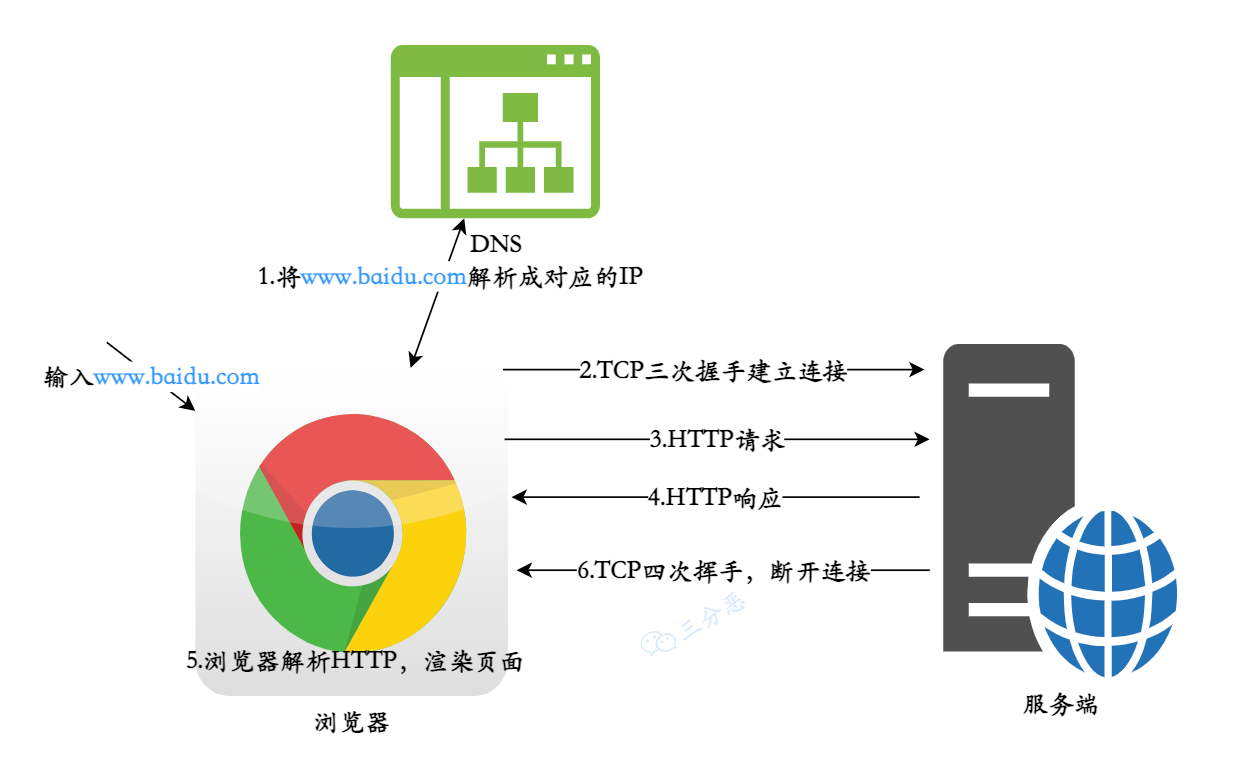
\includegraphics[width=0.95\textwidth]{./Chapter1/q1_1.png}
\caption{浏览器地址输入到显式主页的过程}
\label{fig1_1}
\end{figure}

各个过程使用到的协议如下图\ref{fig1_2} 所示:
\begin{figure}[htbp]
\centering
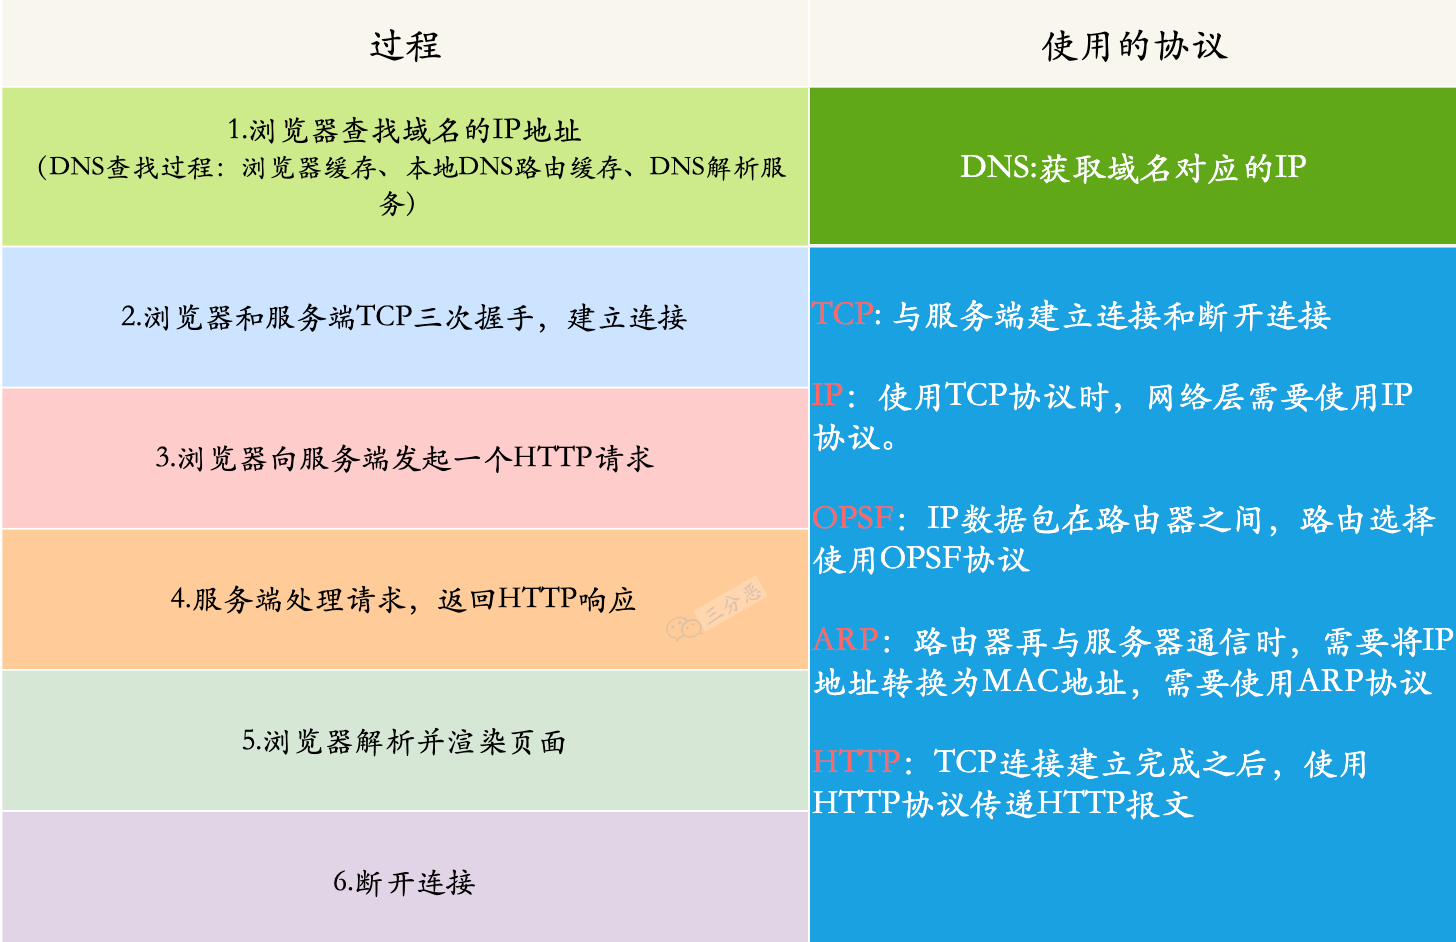
\includegraphics[width=1.0\textwidth]{./Chapter1/q1_2.png}
\caption{每个过程涉及到的协议}
\label{fig1_2}
\end{figure}
\end{solution}

% ----------------------- 问题2 ----------------------
\begin{custom}{问题2}
输入网址到渲染界面过程?
\end{custom}
\begin{solution}
发送http请求--->看本地缓存--->DNS解析出域名对应的IP地址--->TCP/IP五层协议--->可能会有代理(正向代理反向代理)--->TCP连接三次握手 / https认证,加密,解密--->找到端口号--->nignx反向代理将请求分发到具体服务器主机--->mvc框架下从views找到路由--->验证权限--->解析url参数--->看服务器中的缓存--->代码逻辑中获取数据并返回html模板--->服务端发送http响应--->浏览器渲染页面
\end{solution}

% ----------------------- 问题3 ---------------------
\begin{custom}{问题3}
正向代理和反向代理区别?
\end{custom}
\begin{solution}
首先代理是指:客户端主机借助代理服务器访问目标服务器。
\begin{itemize}
\item 客户端 -request-> 代理 -request-> 服务器
\item 客户端 <-response- 代理 <-response- 服务器
\end{itemize}

正向代理:客户端借助代理访问无法访问的服务器,客户端需要配置。

反向代理:服务端借助代理实现负载均衡,客户端无需配置,也不知道自己经过了代理。
\end{solution}

% ---------------------- 问题4 ----------------
\begin{custom}{问题4}
介绍一下CDN?
\end{custom}
\begin{solution}
视频讲解链接:\href{https://www.zhihu.com/zvideo/1338850254489939968}{https://www.zhihu.com/zvideo/1338850254489939968},后续需要文字整理一下。
\end{solution}

% --- 问题5 ---
\begin{custom}{问题5}
cookie跨域
\end{custom}
\begin{solution}
目前还没有写答案,需要更新
\end{solution}

% ------------------ 问题6 ------------------------
\begin{custom}{问题6}
说一下你了解的端口及对应的服务
\end{custom}
\begin{solution}
常用的端口和作用如下图\ref{fig4_1} 所示:
\begin{figure}[!t]
\centering
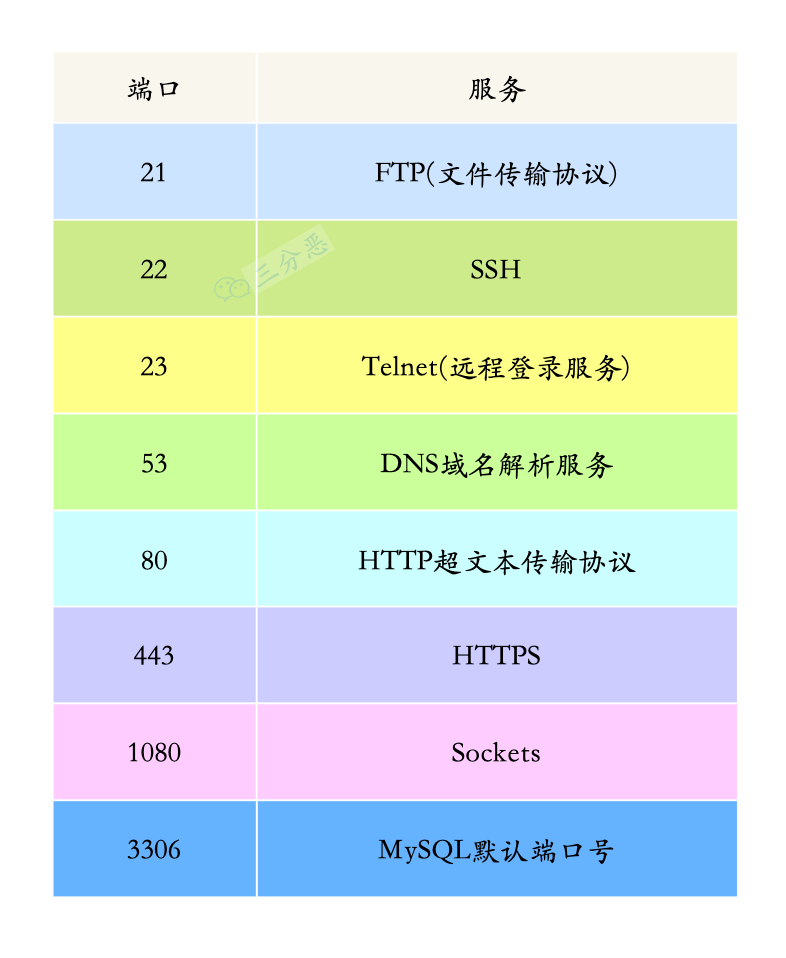
\includegraphics[width=0.75\textwidth]{./Chapter1/q4_1.png}
\caption{常见端口及对应服务}
\label{fig4_1}
\end{figure}

\end{solution}



\chapter{计算机网络体系}
% ------------- 问题 7 --------------
\begin{custom}{问题7}
说下计算机网络体系结构
\end{custom}
\begin{solution}
计算机网络体系结构,一般有 3 种:OSI 七层模型、五层结构、TCP/IP 四层模型,如下图\ref{fig7_1} 所示:

\begin{figure}[htbp]
\centering
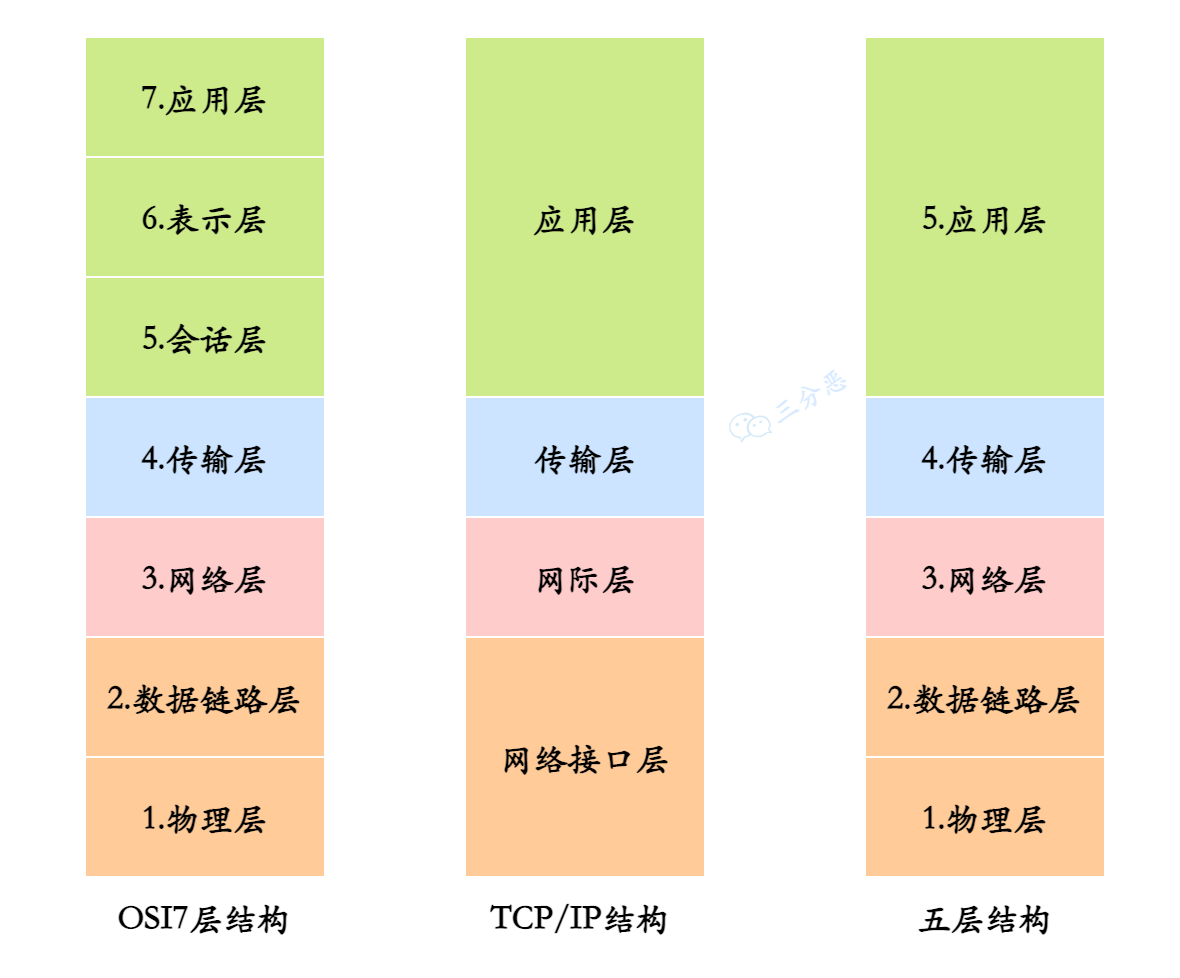
\includegraphics[width=0.75\textwidth]{./Chapter2/q7_1.png}
\caption{3 种计算机网络体系}
\label{fig7_1}
\end{figure}
简单说,OSI 是一个理论上的网络通信模型,TCP/IP 是实际上的网络通信模型,五层结构就是为了介绍网络原理而折中的网络通信模型。

\begin{note} \textbf{OSI 七层模型} \end{note}

OSI 七层模型是国际标准化组织(International Organization for Standardization)制定的一个用于计算机或通信系统间互联的标准体系。
\begin{enumerate}
\item 应用层:通过应用进程之间的交互来完成特定网络应用,应用层协议定义的是应用进程间通信和交互的规则,常见的协议有:HTTP FTP SMTP SNMP DNS.
\item 表示层:数据的表示、安全、压缩。确保一个系统的应用层所发送的信息可以被另一个系统的应用层读取。
\item 会话层:建立、管理、终止会话,是用户应用程序和网络之间的接口。
\item 运输层:提供源端与目的端之间提供可靠的透明数据传输,传输层协议为不同主机上运行的进程提供逻辑通信。
\item 网络层:将网络地址翻译成对应的物理地址,实现不同网络之间的路径选择, 协议有 ICMP, IGMP, IP 等。
\item 数据链路层:在物理层提供比特流服务的基础上,建立相邻结点之间的数据链路。
\item 物理层:建立、维护、断开物理连接。
\end{enumerate}

\begin{note} \textbf{五层体系结构} \end{note}
\begin{enumerate}
\item 应用层:对应于 OSI 参考模型的(应用层、表示层、会话层)。
\item 传输层:对应 OSI 参考模型的的传输层。
\item 网络层:对应 OSI 参考模型的的网络层。
\item 数据链路层:对应 OSI 参考模型的的数据链路层。
\item 物理层:对应 OSI 参考模型的的物理层。
\end{enumerate}

\begin{note} \textbf{TCP/IP 四层结构} \end{note}
\begin{enumerate}
\item 应用层:对应于 OSI 参考模型的(应用层、表示层、会话层)。
\item 传输层: 对应 OSI 的传输层,为应用层实体提供端到端的通信功能,保证了数据包的顺序传送及数据的完整性。
\item 网际层:对应于 OSI 参考模型的网络层,主要解决主机到主机的通信问题。
\item 网络接口层:与 OSI 参考模型的数据链路层、物理层对应。
\end{enumerate}
\end{solution}

% ----------------------- 问题8 ---------------------
\begin{custom}{问题8}
说一下每一层对应的网络协议有哪些?
\end{custom}
\begin{solution}
一张表格总结常见网络协议,如下图\ref{fig8_1} 所示:

\begin{figure}[htbp]
\centering
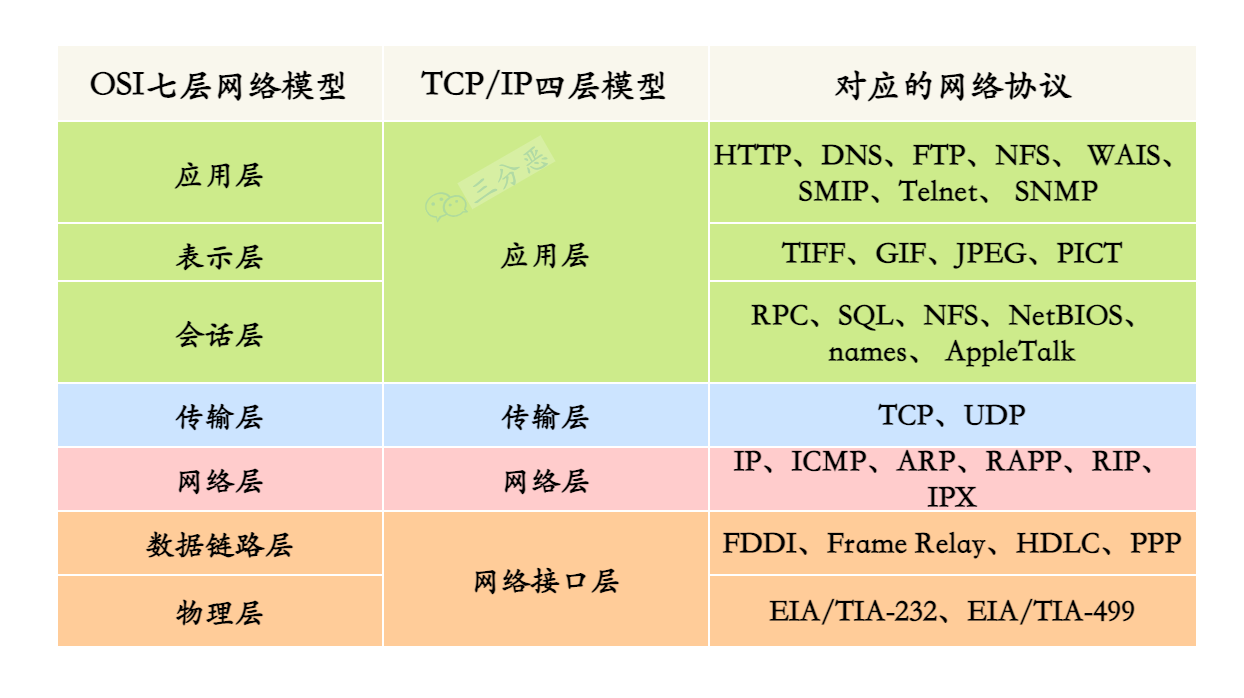
\includegraphics[width=0.95\textwidth]{./Chapter2/q8_1.png}
\caption{计算机网络体系每层对应网络协议}
\label{fig8_1}
\end{figure}
\end{solution}

% -------------------- 问题9 --------------------
\begin{custom}{问题9}
数据在各层之间是怎么传输的呢?
\end{custom}
\begin{solution}
对于发送方而言,从上层到下层层层包装;对于接收方而言,从下层到上层,层层解开包装。
\begin{enumerate}
\item 发送方的\textbf{应用进程}(如 QQ 等某个应用程序)向接收方的应用进程传送数据;
\item AP (application) 先将数据交给本主机的\textbf{应用层},应用层加上本层的控制信息 H5 就变成了下一层的数据单元;
\item \textbf{传输层}收到这个数据单元后,加上本层的控制信息 H4,再交给网络层,成为网络层的数据单元;
\item 到了\textbf{数据链路层},控制信息被分成两部分,分别加到本层数据单元的首部(H2)和尾部(T2);
\item 最后的\textbf{物理层},进行比特流的传输
\end{enumerate}
\end{solution}

上述过程如下图\ref{fig9_1} 所示,这个过程类似写信,写一封信,每到一层,就加一个信封,写一些地址的信息。到了目的地之后,又一层层解封,传向下一个目的地。
\begin{figure}[htbp]
\centering
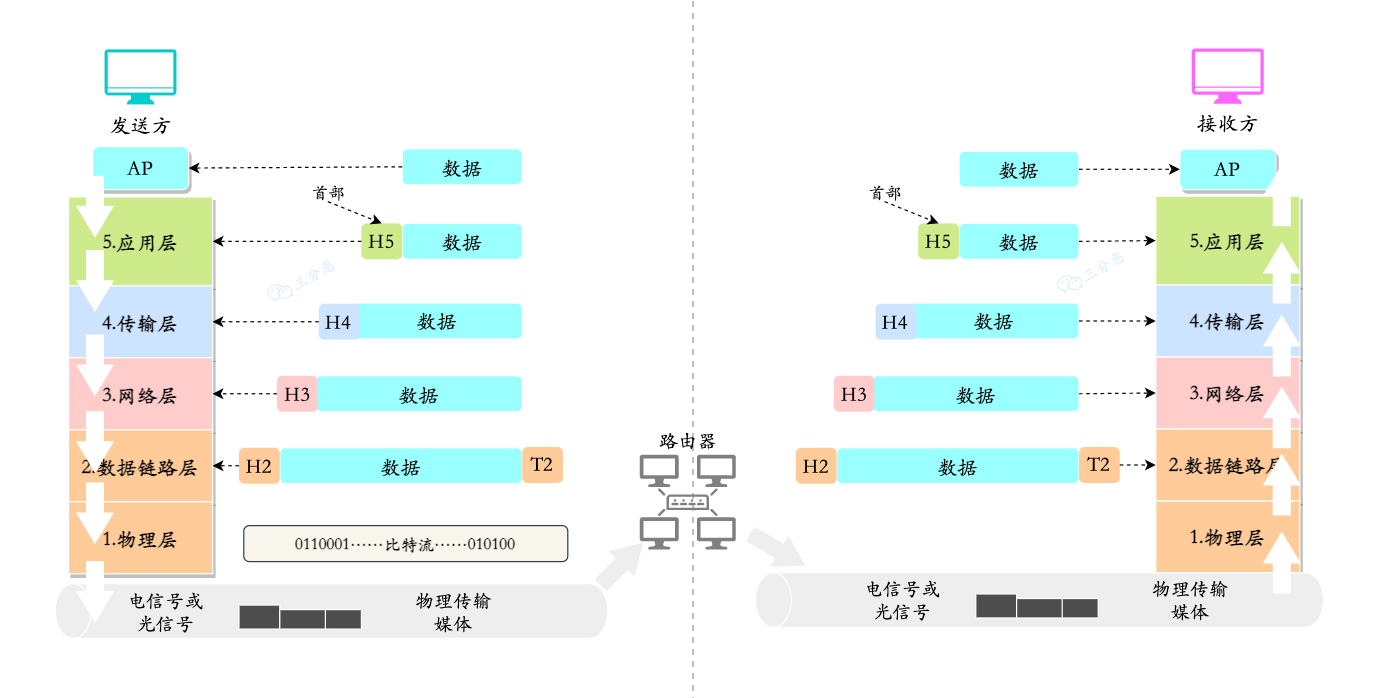
\includegraphics[width=1.0\textwidth]{./Chapter2/q9_1.png}
\caption{计算机网络体系每层对应网络协议}
\label{fig9_1}
\end{figure}

\chapter{应用层对应问题}

% --------------- 问题10 ---------------------
\begin{custom}{问题10}
DNS解析原理和过程?
\end{custom}
\begin{solution}
\begin{note} \textbf{DNS 解析过程} \end{note}
DNS,英文全称是 domain name system,域名解析系统,它的作用也很明确,就是域名和 IP 相互映射。

DNS 的解析过程如下图\ref{fig10_1} 所示:

\begin{figure}[htbp]
\centering
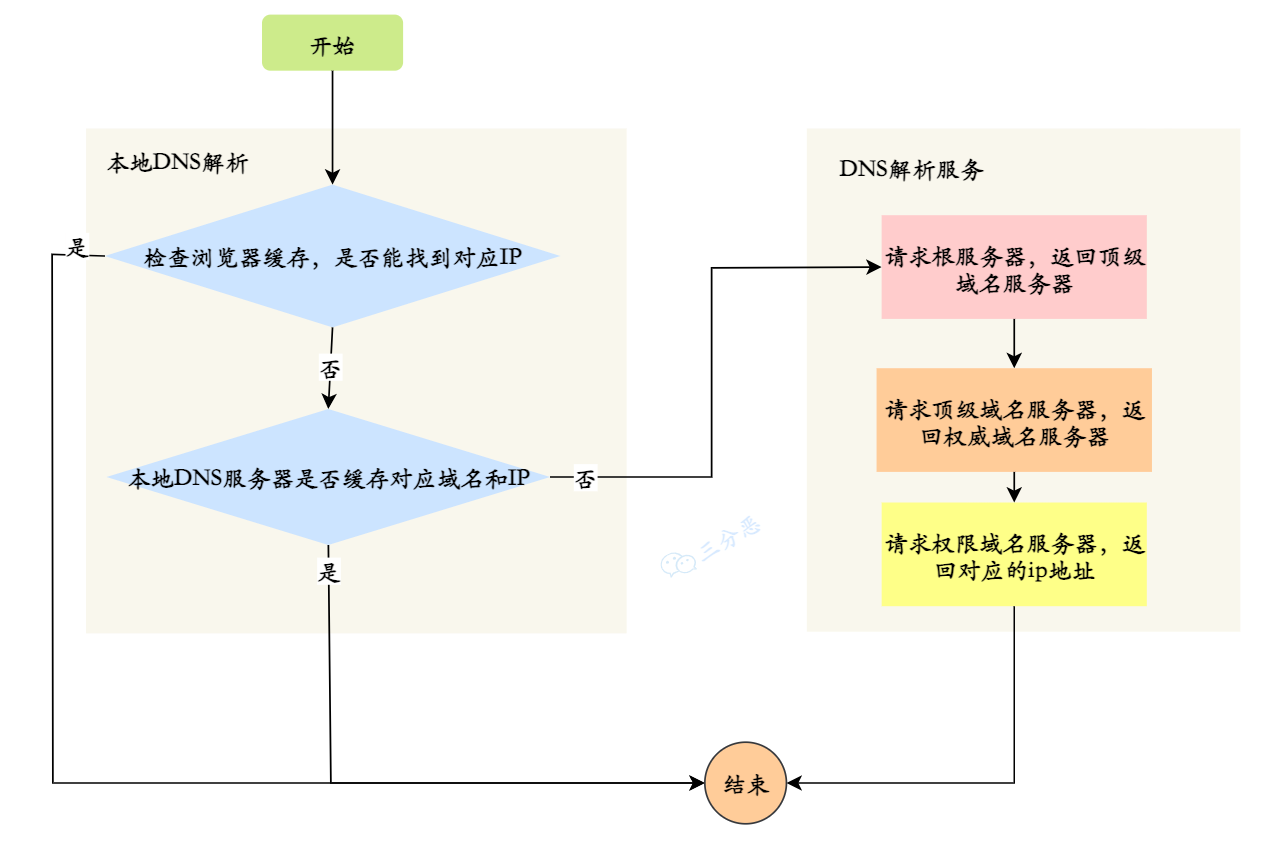
\includegraphics[width=1.0\textwidth]{./Chapter3/q10_1.png}
\caption{计算机网络体系每层对应网络协议}
\label{fig10_1}
\end{figure}

假设你要查询 www.baidu.com 的 IP 地址:
\begin{enumerate}
	\item 首先会查找\textbf{浏览器的缓存},看看是否能找到 www.baidu.com 对应的 IP 地址,找到就直接返回;否则进行下一步。
	\item 将请求发往给\textbf{本地 DNS 服务器},如果查找到也直接返回,否则继续进行下一步;
	\item 本地 DNS 服务器向\textbf{根域名服务器}发送请求,根域名服务器返回负责 com 的顶级域名服务器的 IP 地址的列表。
	\item 本地 DNS 服务器再向其中一个\textbf{负责 com 的顶级域名服务器}发送一个请求,返回负责 baidu.com 的权限域名服务器的 IP 地址列表。
	\item 本地 DNS 服务器再向其中一个\textbf{权限域名服务器}发送一个请求,返回 www.baidu.com 所对应的IP地址
\end{enumerate}

上面提到了本地递归式地查询了:权限域名服务器 --> 顶级域名服务器 --> 根域名服务器,它们的关系如下图\ref{fig10_2} 所示:
\begin{figure}[htbp]
\centering
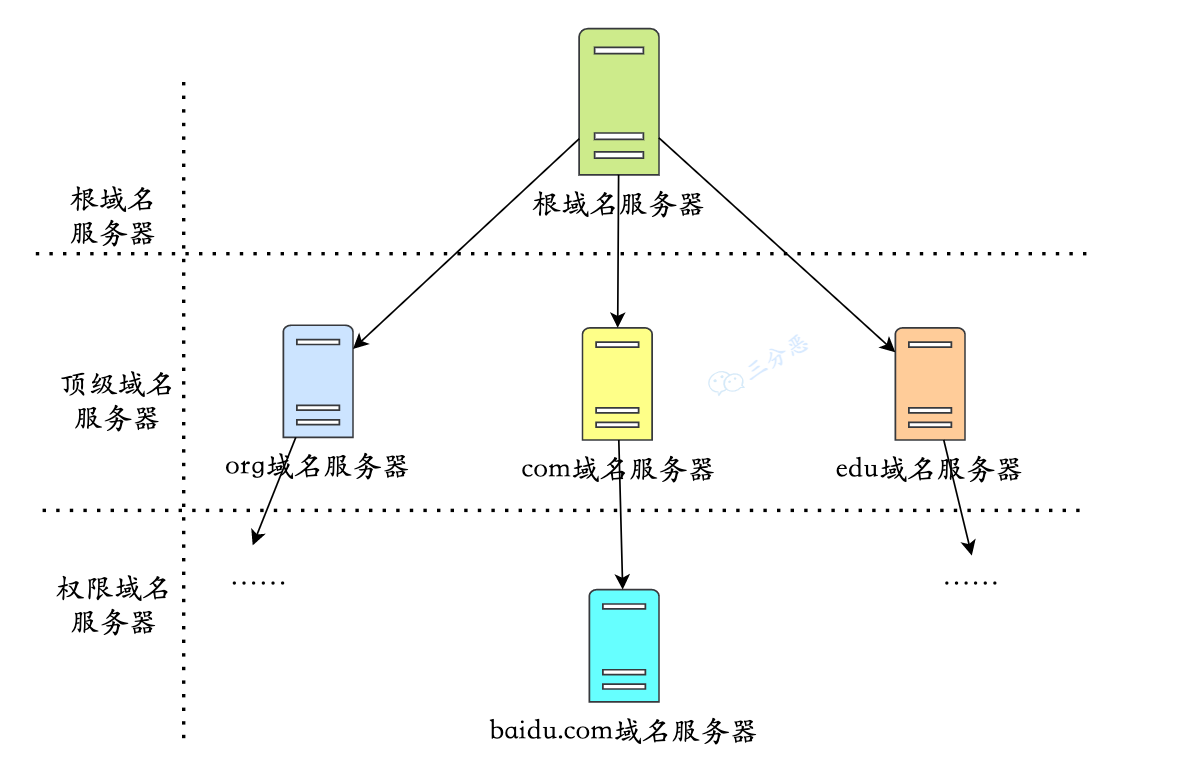
\includegraphics[width=0.8\textwidth]{./Chapter3/q10_2.png}
\caption{计算机网络体系每层对应网络协议}
\label{fig10_2}
\end{figure}

另外,对上面的本地 DNS 服务器和权威服务器做一个概念上的补充,如下所示:
\begin{myDefinition}{本地 DNS 服务器}{example}

本地 DNS 一般是指你电脑上网时 IPv4 或者 IPv6 设置中填写的那个 DNS,这个有可能是手工指定的或者是 DHCP 自动分配的。如果你的电脑是直连运营商网络,一般默认设置情况下 DNS 为 DHCP 分配到的运营商的服务器地址。

如果你的电脑和运营商之间还加了无线或者有线路由,那极有可能路由器本身还内置了一个 DNS 转发器,这玩意的作用是将发往他所有的 DNS 请求转发到上层 DNS。此时由于路由器本身也接管了下挂电脑的 DHCP 服务,所以它分配给下面电脑的 DNS 地址就是它自身,所以你能看到电脑的 DNS 分配到的可能是 192.168.1.1。实际上就是路由器自身,而路由器的 DNS 转发器将请求转发到上层 ISP 的 DNS。所以这里说 DNS 是局域网或者是运营商的都可以(因为最终都是转发到运营商,小细节不用纠结)。
\end{myDefinition}

\begin{myDefinition}{权威服务器}{example}
权威服务器是特殊的DNS服务器,所谓的权威是针对特定域名来说的。所以一般会说某某域名的权威DNS是谁,不能单纯的抛离域名问权威DNS是谁。是域名商在管理,负责解析在他这里购买的域名的权威解析(当然也存在此处购买域名挂靠别处权威的情况。同样,不要纠结于小细节,意思懂了就行。如果要了解原理请查找一下NS记录这个名词)。
\end{myDefinition}

\begin{note} \textbf{DNS 解析原理} \end{note}
上面已经详细说明了解析的步骤,下面是上述每一步涉及到的理论:
\begin{enumerate} 
	\item 浏览器输入域名, 操作系统\textbf{检查自己本地的 hosts 文件是否有这个网址映射关系},如果有,就先调度这个 IP 地址映射,完成域名解析;如果没有,则\textbf{查找本地 DNS 解析器缓存}。
	\item 如果还没有,则\textbf{找到 TCP/IP 参数中设置的首选 DNS 服务器},DNS 服务器查询域名(具有权威性);如果此域名不由 DNS 服务器区域解析,但该服务器缓存了网址映射关系(则没有权威性)。
	\item 如果查询都失效,则\textbf{查看本地 DNS 服务器是否开转发模式,如未开,则把请求发至根服务器。}根服务器判断这个域名谁授权管理,并返回一个负责该顶级域名服务器的IP。
	\item 本地 DNS 服务器收到 IP 信息后,将会联系负责 .com 域的这台服务器。如果这台服务器无法解析,就会找到下一级 DNS 服务器地址 (http://qq.com) 给本地 DNS 服务器。重复以上操作,直到找到http://www.qq.com 主机。
	\item 如果是转发模式,此 DNS 服务器就会把请求转发至上一级 DNS 服务器,上一级服务器进行解析。如果不行,就上上级,以此循环。
\end{enumerate}
\end{solution}

%--------------- 问题11 -------------------
\begin{custom}{问题11}
说说 WebSocket 与 Socket 的区别
\end{custom}
\begin{solution}
Socket 一个是网编编程的标准接口,而 WebSocket 则是应用层通信协议。

\begin{itemize}
	\item Socket 其实就是等于:IP 地址 + 端口 + 协议。具体来说,Socket 是一套标准,它完成了对 TCP/IP 的高度封装,屏蔽网络细节,以方便开发者更好地进行网络编程。
	\item WebSocket 是一个持久化的协议,它是伴随 H5 而出的协议,用来解决 http 不支持持久化连接的问题
\end{itemize}

\end{solution}

%------------- 问题12 -----------------
\begin{custom}{问题12}
HTTP 请求的过程与原理?
\end{custom}

\begin{solution}
HTTP 协议定义了浏览器怎么向服务器请求文档,以及服务器怎么把文档传给浏览器。HTTP 请求过程如下图\ref{fig12_1} 所示
\begin{figure}[!h]
\centering
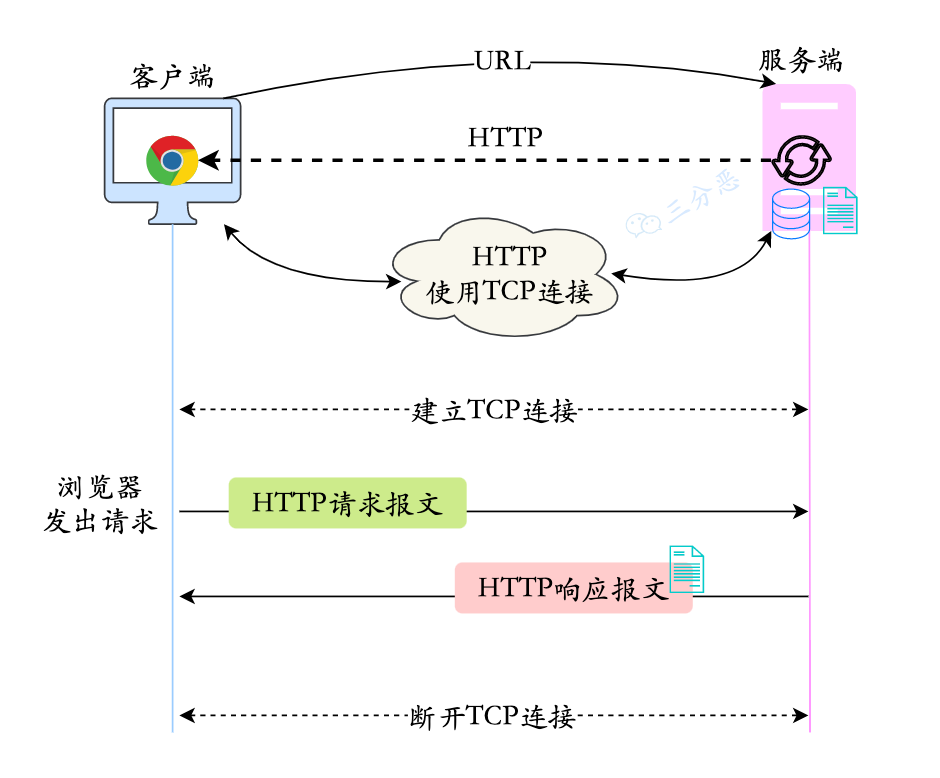
\includegraphics[width=0.6\textwidth]{./Chapter3/q12_1.png}
\caption{HTTP 请求过程}
\label{fig12_1}
\end{figure}

在这个过程中:
\begin{itemize}
	\item 每个服务器都有一个进程,它不断监听 TCP 的端口 80,以便发现是否有浏览器向它发出连接建立请求;
	\item 监听到连接请求,就会建立 TCP 连接;
	\item 浏览器向服务器发出浏览某个页面的请求,服务器接着就返回所请求的页面作为响应;
	\item 最后,释放 TCP 连接。
\end{itemize}
在浏览器和服务器之间的请求和响应的交互,必须按照规定的格式和遵循一定的规则,这些格式和规则就是超文本传输协议 HTTP。 PS:这道题和上面浏览器输入网址发生了什么那道题大差不差。
\end{solution}

%---------- 问题14 ---------------
\begin{custom}{问题14}
说说 HTTP 常用的状态码及其含义?
\end{custom}
\begin{solution}
\href{https://www.runoob.com/http/http-status-codes.html}{HTTP状态码}首先应该知道个大概的分类:
\begin{itemize}
	\item 1XX:信息性状态码
	\item 2XX:成功状态码
	\item 3XX:重定向状态码
	\item 4XX:客户端错误状态码
	\item 5XX:服务端错误状态码
\end{itemize}
几个常用的状态码如下图\ref{fig14_1} 所示,也应该记住:
\begin{figure}[htbp]
\centering
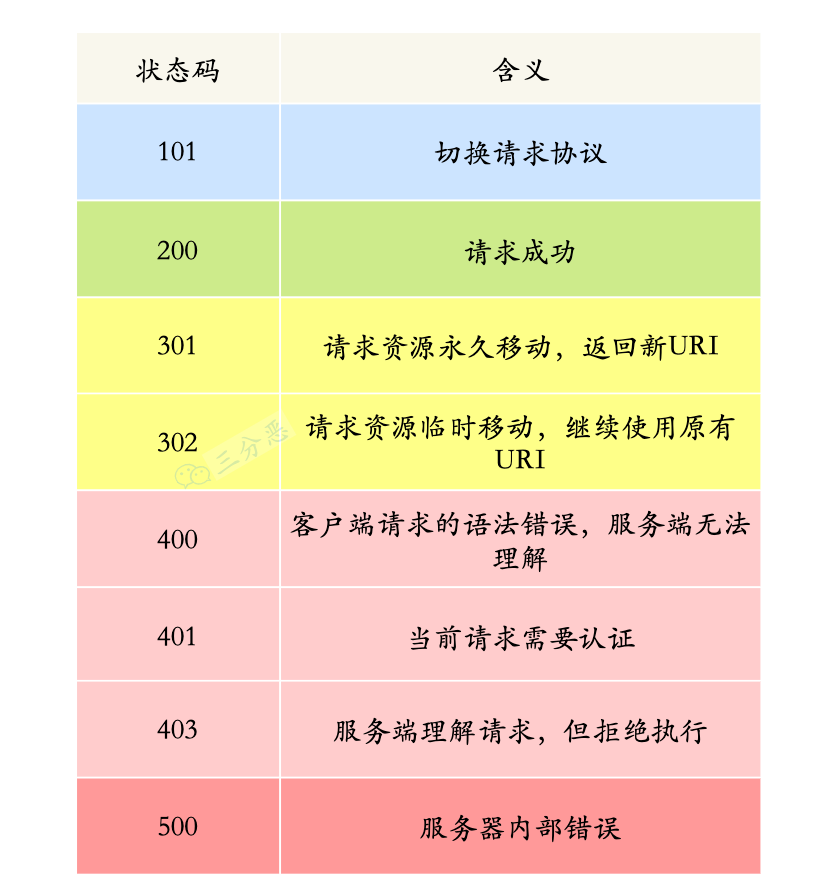
\includegraphics[width=0.65\textwidth]{./Chapter3/q14_1.png}
\caption{常见的状态码}
\label{fig14_1}
\end{figure}
\end{solution}

%---------------- 问题15 ----------------
\begin{custom}{问题15}
说一下HTTP的报文结构?
\end{custom}

\begin{solution}
HTTP 报文有两种,HTTP 请求报文和 HTTP 响应报文,大致结构如下图\ref{fig15_1} 所示:
\begin{figure}[htbp]
\centering
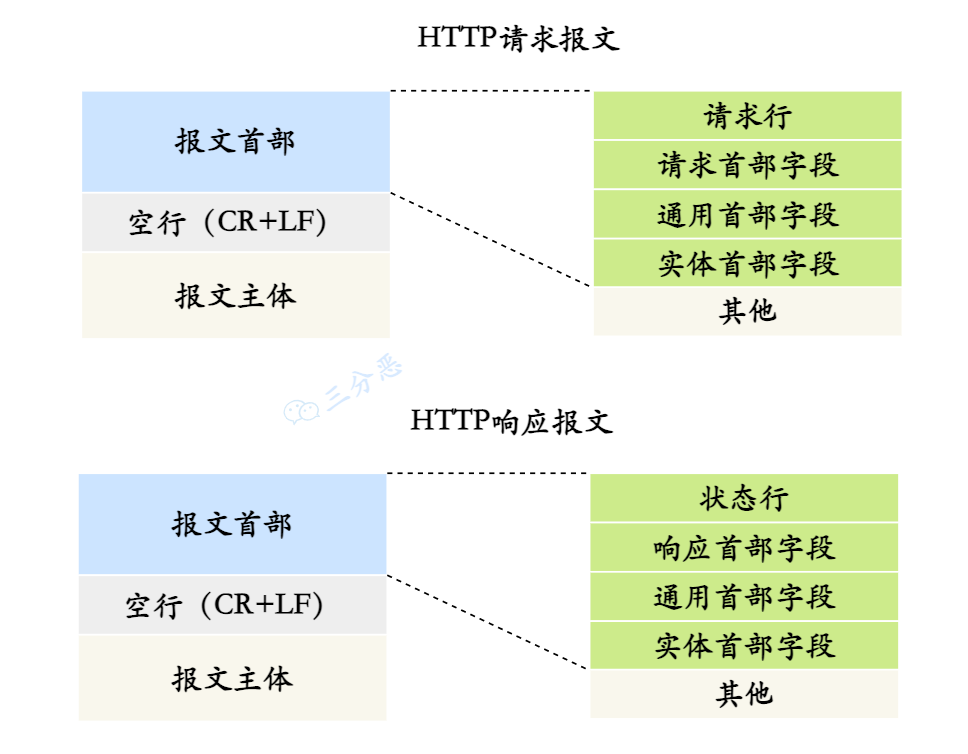
\includegraphics[width=0.7\textwidth]{./Chapter3/q15_1.png}
\caption{HTTP 请求报文和响应报文的大致结构}
\label{fig15_1}
\end{figure}

\begin{note} \textbf{HTTP 请求报文} \end{note}
HTTP 请求报文的格式如下:

\begin{lstlisting}
GET / HTTP/1.1                                                   
User-Agent: Mozilla/5.0 (Macintosh; Intel Mac OS X 10_10_5)      
Accept: */*                                                       
\end{lstlisting}

HTTP 请求报文的第一行叫做请求行,后面的行叫做首部行,首部行后还可以跟一个实体主体。请求首部之后有一个空行,这个空行不能省略,它用来划分首部与实体。

请求行包含三个字段:
\begin{itemize}
	\item 方法字段:包括 POST、GET 等请方法。
	\item URL 字段
	\item HTTP 版本字段。
\end{itemize}

\begin{note} \textbf{响应报文} \end{note}
HTTP 响应报文的格式如下:
\begin{lstlisting}
HTTP/1.0 200 OK                                    

Content-Type: text/plain
Content-Length: 137582                             
Expires: Thu, 05 Dec 1997 16:00:00 GMT             
Last-Modified: Wed, 5 August 1996 15:55:28 GMT     
Server: Apache 0.84
<html>
  <body>Hello World</body>
</html>                                                     
\end{lstlisting}

\begin{itemize}
	\item 状态行包含了三个字段:协议版本字段、状态码和相应的状态信息。
	\item 首部行首部可以分为四种首部,请求首部、响应首部、通用首部和实体首部。通用首部和实体首部在请求报文和响应报文中都可以设置,区别在于请求首部和响应首部。
	\begin{itemize}
		\item 常见的请求首部有 Accept 可接收媒体资源的类型、Accept-Charset 可接收的字符集、Host 请求的主机名。
		\item 常见的响应首部有 ETag 资源的匹配信息,Location 客户端重定向的 URI。
		\item 常见的通用首部有 Cache-Control 控制缓存策略、Connection 管理持久连接。
		\item 常见的实体首部有 Content-Length 实体主体的大小、Expires 实体主体的过期时间、Last-Modified 资源的最后修改时间。
	\end{itemize}
	\item 实体部分是报文的主要部分,它包含了所请求的对象。
\end{itemize}
\end{solution}

% ------------- 问题16 --------------
\begin{custom}{问题16}
URI 和 URL 有什么区别?
\end{custom}

\begin{solution}
URI 是 URL 的一个子集,如下图\ref{fig16_1} 所示:
\begin{figure}[htbp]
\centering
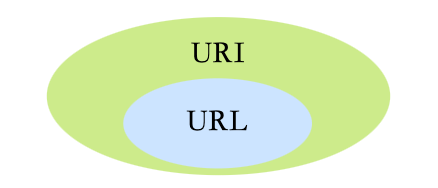
\includegraphics[width=0.6\textwidth]{./Chapter3/q16_1.png}
\caption{URI 和 URL 关系}
\label{fig16_1}
\end{figure}

它们的主要区别在于,URL 除了提供了资源的标识,还提供了资源访问的方式。这么比喻,URI 像是身份证,可以唯一标识一个人;而 URL 更像一个住址,可以通过 URL 找到这个人——人类住址协议://地球/中国/北京市/海淀区/xx职业技术学院/14号宿舍楼/525号寝/张三.男。
\begin{itemize}
	\item URI,统一资源标识符(Uniform Resource Identifier, URI),标识的是 Web 上每一种可用的资源,如 HTML 文档、图像、视频片段、程序等都是由一个 URI 进行标识的。
	\item URL,统一资源定位符(Uniform Resource Location),它是 URI 的一种子集,主要作用是提供资源的路径。
\end{itemize}
\end{solution}

%------------- 问题17 ---------------
\begin{custom}{问题17}
HTTP 有哪些请求方式?
\end{custom}
\begin{solution}
这里的请求方式是指报文的类型,如下图\ref{fig17_1} 所示:
\begin{figure}[!h]
\centering
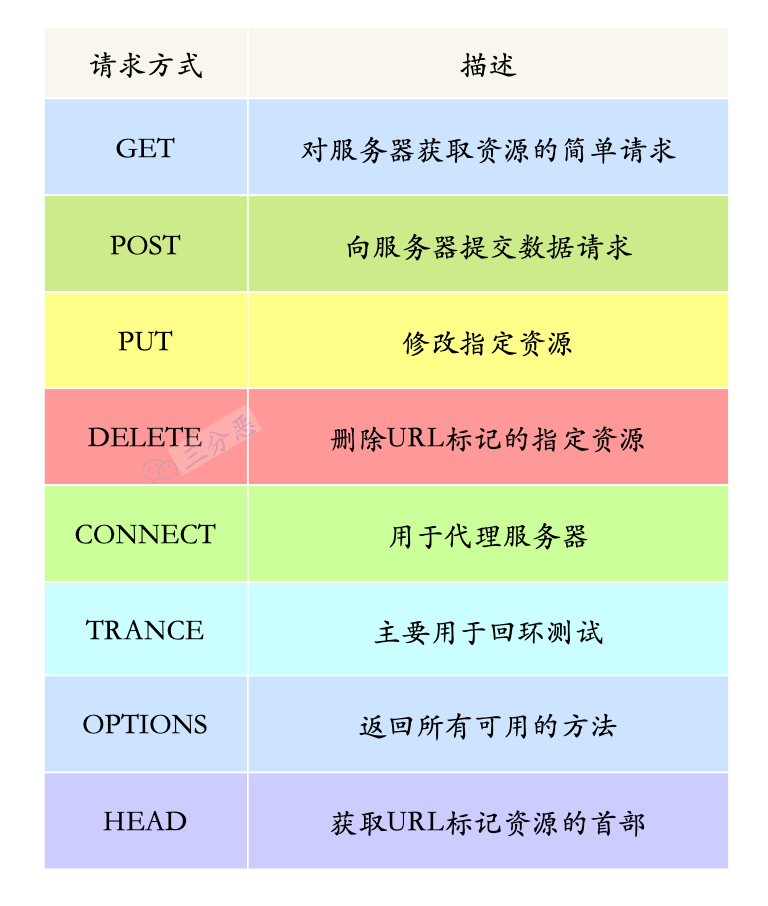
\includegraphics[width=0.7\textwidth]{./Chapter3/q17_1.png}
\caption{各种请求关键字}
\label{fig17_1}
\end{figure}
其中,POST、DELETE、PUT、GET的含义分别对应我们最熟悉的增、删、改、查。
\end{solution}
\newpage
%------------ 问题18 ------------------
\begin{custom}{问题18}
说⼀下 GET 和 POST 的区别?
\end{custom}
\begin{solution}
可以从以下几个方面来说明 GET 和 POST 的区别,如下图\ref{fig18_1} 所示:
\begin{figure}[htbp]
\centering
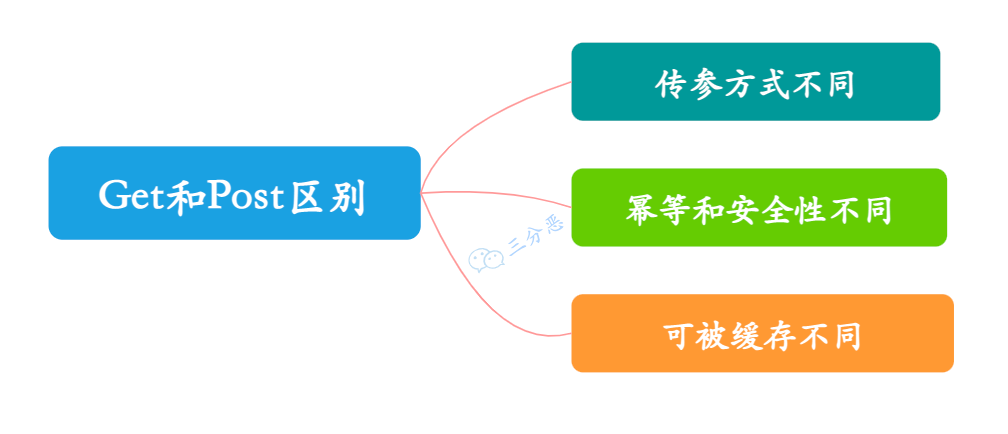
\includegraphics[width=0.7\textwidth]{./Chapter3/q18_1.png}
\caption{GET 和 POST 区别}
\label{fig18_1}
\end{figure}
具体来说
\begin{itemize}
	\item 从 HTTP 报文层面来看,GET 请求将信息放在 URL,POST 将请求信息放在请求体中。这一点使得 GET 请求携带的数据量有限,因为 URL 本身是有长度限制的,而 POST 请求的数据存放在报文体中,因此对大小没有限制。而且从形式上看,GET 请求把数据放 URL 上不太安全,而 POST 请求把数据放在请求体里想比较而言安全一些。
	\item 从数据库层面来看,GET 符合幂等性和安全性,而 POST 请求不符合。这个其实和 GET/POST 请求的作用有关。按照 HTTP 的约定,GET 请求用于查看信息,不会改变服务器上的信息;而 POST 请求用来改变服务器上的信息。正因为 GET 请求只查看信息,不改变信息,对数据库的一次或多次操作获得的结果是一致的,认为它符合幂等性。安全性是指对数据库操作没有改变数据库中的数据。
	\item 从其他层面来看,GET 请求能够被缓存,GET 请求能够保存在浏览器的浏览记录里,GET 请求的 URL 能够保存为浏览器书签。这些都是 POST 请求所不具备的。缓存是 GET 请求被广泛应用的根本,他能够被缓存也是因为它的幂等性和安全性,除了返回结果没有其他多余的动作,因此绝大部分的 GET 请求都被 CDN 缓存起来了,大大减少了 Web 服务器的负担。
\end{itemize}

\end{solution}

% --------- 问题19 --------------
\begin{custom}{问题19}
PUT和POST有什么区别?
\end{custom}
\begin{solution}
xxxxxxxxxxxxxxxxxxxxxx
\end{solution}

% --------- 问题20 --------------
\begin{custom}{问题20}
GET 的长度限制是多少?
\end{custom}
\begin{solution}
HTTP 中的 GET 方法是通过 URL 传递数据的,但是 URL 本身其实并没有对数据的长度进行限制,真正限制 GET 长度的是浏览器。

例如 IE 浏览器对 URL 的最大限制是 2000 多个字符,大概 2kb 左右,像 Chrome、Firefox 等浏览器支持的 URL 字符数更多,其中 FireFox 中 URL 的最大长度限制是 65536 个字符,Chrome 则是 8182个字符。

这个长度限制也不是针对数据部分,而是针对整个 URL。
\end{solution}

% --------- 问题21 --------------
\begin{custom}{问题21}
说下 HTTP/1.0,1.1,2.0 的区别
\end{custom}
\begin{solution}
关键需要记住 HTTP/1.0 默认是短连接,可以强制开启,HTTP/1.1 默认长连接,HTTP/2.0 采用多路复用。
\begin{note} \textbf{HTTP/1.0} \end{note}
默认使用短连接,每次请求都需要建立一个 TCP 连接。它可以设置Connection: keep-alive 这个字段,强制开启长连接。

\begin{note} \textbf{HTTP/1.1} \end{note}
\begin{itemize}
	\item 引入了持久连接,即 TCP 连接默认不关闭,可以被多个请求复用。
	\item 分块传输编码,即服务端每产生一块数据,就发送一块,用” 流模式” 取代” 缓存模式”。
	\item 管道机制,即在同一个 TCP 连接里面,客户端可以同时发送多个请求。
\end{itemize}

\begin{note} \textbf{HTTP/2.0} \end{note}
\begin{itemize}
	\item 二进制协议,1.1 版本的头信息是文本(ASCII 编码),数据体可以是文本或者二进制;2.0 中,头信息和数据体都是二进制。
	\item 完全多路复用,在一个连接里,客户端和浏览器都可以同时发送多个请求或回应,而且不用按照顺序一一对应。
	\item 报头压缩,HTTP 协议不带有状态,每次请求都必须附上所有信息。Http/2.0 引入了头信息压缩机制,使用 gzip 或 compress 压缩后再发送。
	\item 服务端推送,允许服务器未经请求,主动向客户端发送资源。
\end{itemize}
\end{solution}

% --------- 问题22 --------------
\begin{custom}{问题22}
HTTP/3了解吗?
\end{custom}
\begin{solution}

HTTP/3 主要有两大变化,\textbf{传输层基于 UDP}、使用 \textbf{QUIC 保证 UDP 可靠性}。

HTTP/2 存在的一些问题,比如重传等等,都是由于 TCP 本身的特性导致的,所以 HTTP/3 在 QUIC 的基础上进行发展而来,QUIC(Quick UDP Connections)直译为快速 UDP 网络连接,底层使用UDP 进行数据传输。

HTTP/3 主要有这些特点:

\begin{itemize}
	\item 使用 UDP 作为传输层进行通信
	\item 在 UDP 的基础上 QUIC 协议保证了 HTTP/3 的安全性,在传输的过程中就完成了 TLS 加密握手
	\item HTTPS 要建立一个连接,要花费 6 次交互,先是建立三次握手,然后是 TLS/1.3 的三次握手。QUIC 直接把以往的 TCP 和 TLS/1.3 的 6 次交互合并成了 3 次,减少了交互次数。
	\item QUIC 有一套自己的机制可以保证传输的可靠性的。当某个流发生丢包时,只会阻塞这个流,其他流不会受到影响。
\end{itemize}

我们拿一张图\ref{fig22_1} 看一下 HTTP 协议的变迁:
\begin{figure}[htbp]
\centering
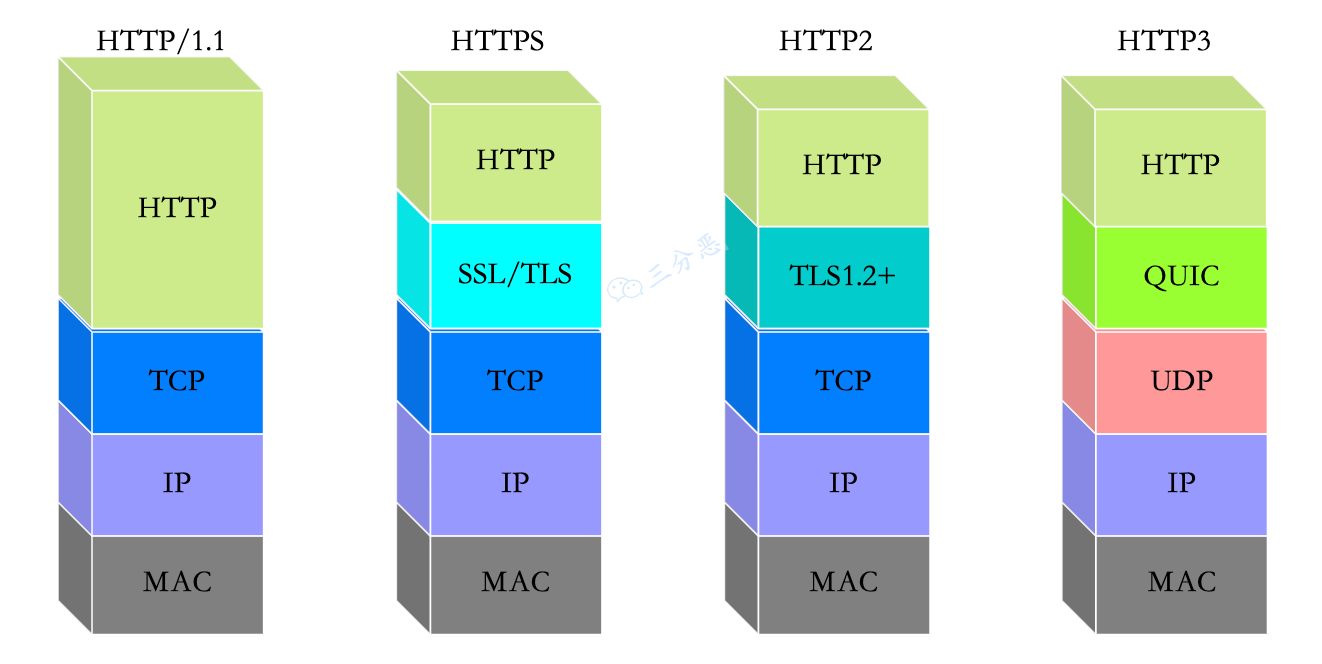
\includegraphics[width=0.7\textwidth]{./Chapter3/q22_1.png}
\caption{HTTP 变迁}
\label{fig22_1}
\end{figure}
\end{solution}

% --------- 问题23 --------------
\begin{custom}{问题19}
HTTP 如何实现长连接?在什么时候会超时?
\end{custom}
\begin{solution}
\begin{note} \textbf{什么是 HTTP 的长连接?} \end{note}

\begin{itemize}
	\item HTTP 分为长连接和短连接,本质上说的是 TCP 的长短连接。TCP 连接是一个双向的通道,它是可以保持一段时间不关闭的,因此 TCP 连接才具有真正的长连接和短连接这一说法。
	\item TCP 长连接可以复用一个 TCP 连接,来发起多次的 HTTP 请求,这样就可以减少资源消耗,比如一次请求 HTML,如果是短连接的话,可能还需要请求后续的 JS/CSS。
\end{itemize}

\begin{note} \textbf{如何设置长连接?} \end{note}
通过在头部(请求和响应头)设置 Connection 字段指定为keep-alive,HTTP/1.0 协议支持,但是是默认关闭的,从 HTTP/1.1 以后,连接默认都是长连接。

\begin{note} \textbf{在什么时候会超时呢?} \end{note}

\begin{itemize}
	\item HTTP 一般会有 httpd 守护进程,里面可以设置 keep-alive timeout,当 tcp 连接闲置超过这个时间就会关闭,也可以在 HTTP 的 header 里面设置超时时间。

	\item TCP 的 keep-alive 包含三个参数,支持在系统内核的 net.ipv4 里面设置;当 TCP 连接之后,闲置了 tcp\_keepalive\_time ,则会发生侦测包,如果没有收到对方的 ACK,那么会每隔 tcp\_keepalive\_intvl 再发一次,直到发送了 tcp\_keepalive\_probes,就会丢弃该连接。
\end{itemize}
\begin{lstlisting}
tcp_keepalive_intvl = 15
tcp_keepalive_probes = 5
tcp_keepalive_time = 1800
\end{lstlisting}

\end{solution}

% --------- 问题24 --------------
\begin{custom}{问题24}
说说HTTP 与 HTTPS 有哪些区别?
\end{custom}
\begin{solution}
\begin{enumerate}
	\item HTTP 是超文本传输协议,信息是明文传输,存在安全风险的问题。HTTPS 则解决 HTTP 不安全的缺陷,在 TCP 和 HTTP 网络层之间加入了 SSL/TLS 安全协议,使得报文能够加密传输。
	\item HTTP 连接建立相对简单, TCP 三次握手之后便可进行 HTTP 的报文传输。而 HTTPS 在 TCP 三次握手之后,还需进行 SSL/TLS 的握手过程,才可进行加密报文传输。
	\item HTTP 的端口号是 80,HTTPS 的端口号是 443。
	\item HTTPS 协议需要向 CA(证书权威机构)申请数字证书,来保证服务器的身份是可信的。
\end{enumerate}
\end{solution}

% --------- 问题25 --------------
\begin{custom}{问题25}
为什么要用HTTPS?解决了哪些问题?
\end{custom}
\begin{solution}
因为 HTTP 是明文传输,存在安全上的风险:
\begin{itemize}
	\item 窃听风险,比如通信链路上可以获取通信内容,用户账号被盗。
	\item 篡改风险,比如强制植入垃圾广告,视觉污染。
	\item 冒充风险,比如冒充淘宝网站,用户金钱损失。
\end{itemize}

所以引入了 HTTPS,HTTPS 在 HTTP 与 TCP 层之间加入了 SSL/TLS 协议,可以很好的解决了这些风险:
\begin{itemize}
	\item 信息加密:交互信息无法被窃取。
	\item 校验机制:无法篡改通信内容,篡改了就不能正常显示。
	\item 身份证书:能证明淘宝是真淘宝。
\end{itemize}
所以通过加入下图\ref{fig25_1} 所示的 SSL/TLS 协议,是能保证通信是安全的。
\begin{figure}[htbp]
\centering
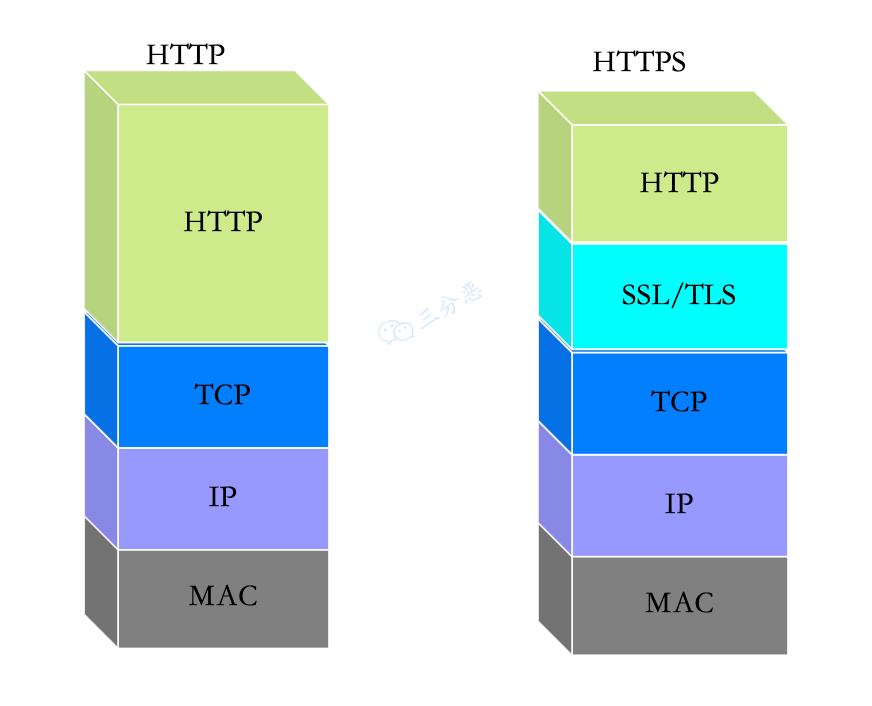
\includegraphics[width=0.6\textwidth]{./Chapter3/q25_1.png}
\caption{SSL/TSL 保证通信安全}
\label{fig25_1}
\end{figure}
\end{solution}

%------------- 问题26 ------------------
\begin{custom}{问题26}
HTTPS工作流程是怎样的?
\end{custom}

\begin{solution}
这道题有几个要点:\textbf{公私钥、数字证书、加密、对称加密、非对称加密}。

HTTPS 主要工作流程:
\begin{enumerate}
	\item 客户端发起 HTTPS 请求,连接到服务端的 443 端口。
	\item 服务端有一套数字证书(证书内容有公钥、证书颁发机构、失效日期等)。
	\item 服务端将自己的数字证书发送给客户端(公钥在证书里面,私钥由服务器持有)。
	\item 客户端收到数字证书之后,会验证证书的合法性。如果证书验证通过,就会生成一个随机的对称密钥,用证书的公钥加密。
	\item 客户端将公钥加密后的密钥发送到服务器。
	\item 服务器接收到客户端发来的密文密钥之后,用自己之前保留的私钥对其进行非对称解密,解密之后就得到客户端的密钥,然后用客户端密钥对返回数据进行对称加密,酱紫传输的数据都是密文啦。
	\item 服务器将加密后的密文返回到客户端。
	\item 客户端收到后,用自己的密钥对其进行对称解密,得到服务器返回的数据。
\end{enumerate}
工作流程如下图\ref{fig26_1} 所示:
\begin{figure}[htbp]
\centering
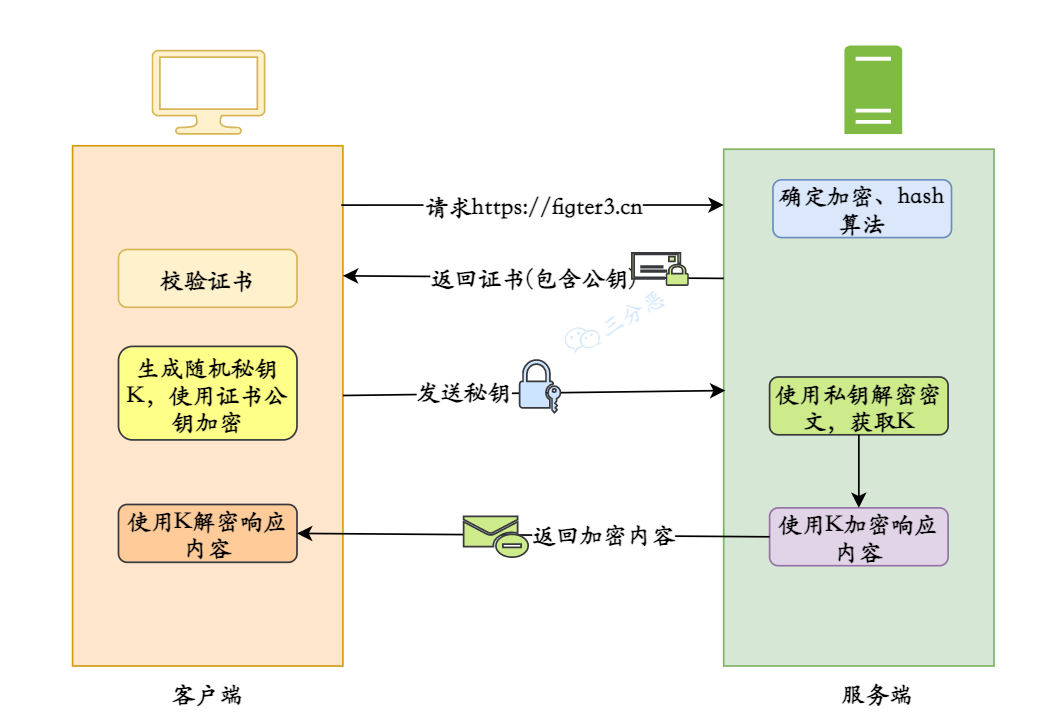
\includegraphics[width=0.7\textwidth]{./Chapter3/q26_1.png}
\caption{HTTPS 主要工作流程}
\label{fig26_1}
\end{figure}

这里还画了一张更详尽的图:
\begin{figure}[htbp]
\centering
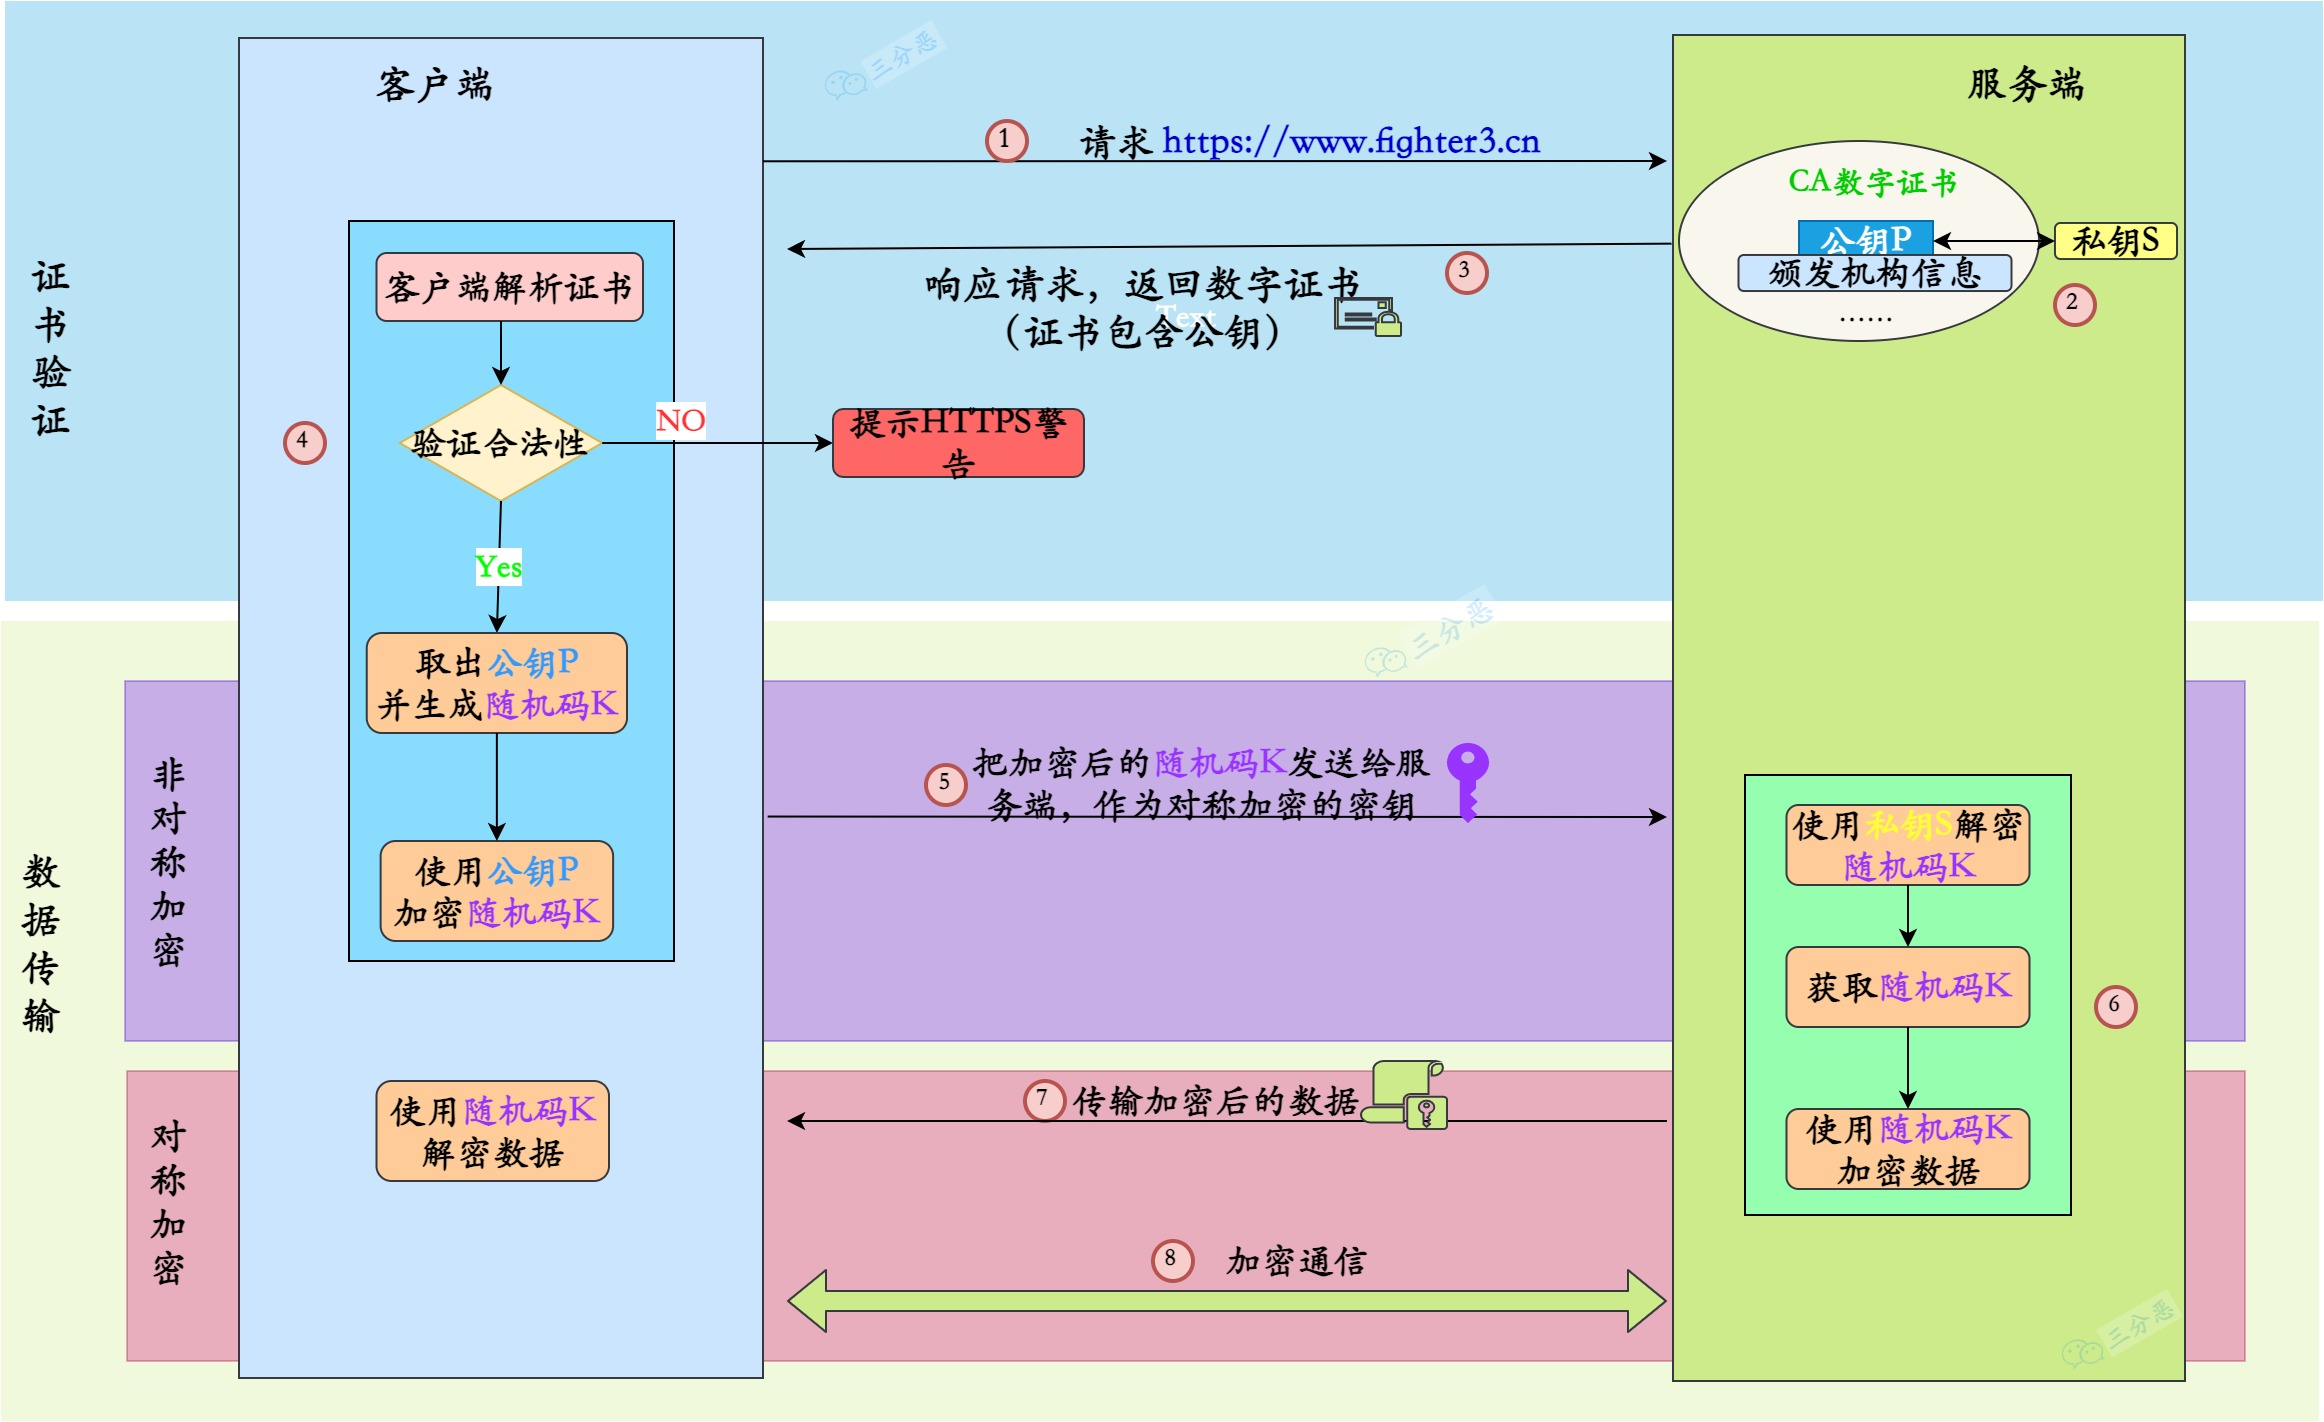
\includegraphics[width=0.7\textwidth]{./Chapter3/q26_2.png}
\caption{详细的 HTTPS 流程}
\label{fig26_2}
\end{figure}

\end{solution}

%------------- 问题27 -------------------
\begin{custom}{问题27}
客户端怎么去校验证书的合法性?
\end{custom}

\begin{solution}
首先,服务端的证书从哪来的呢?

为了让服务端的公钥被大家信任,服务端的证书都是由 CA (Certificate Authority,证书认证机构)签名的,CA 就是网络世界里的公安局、公证中心,具有极高的可信度,所以由它来给各个公钥签名,信任的一方签发的证书,那必然证书也是被信任的。

\begin{figure}[htbp]
\centering
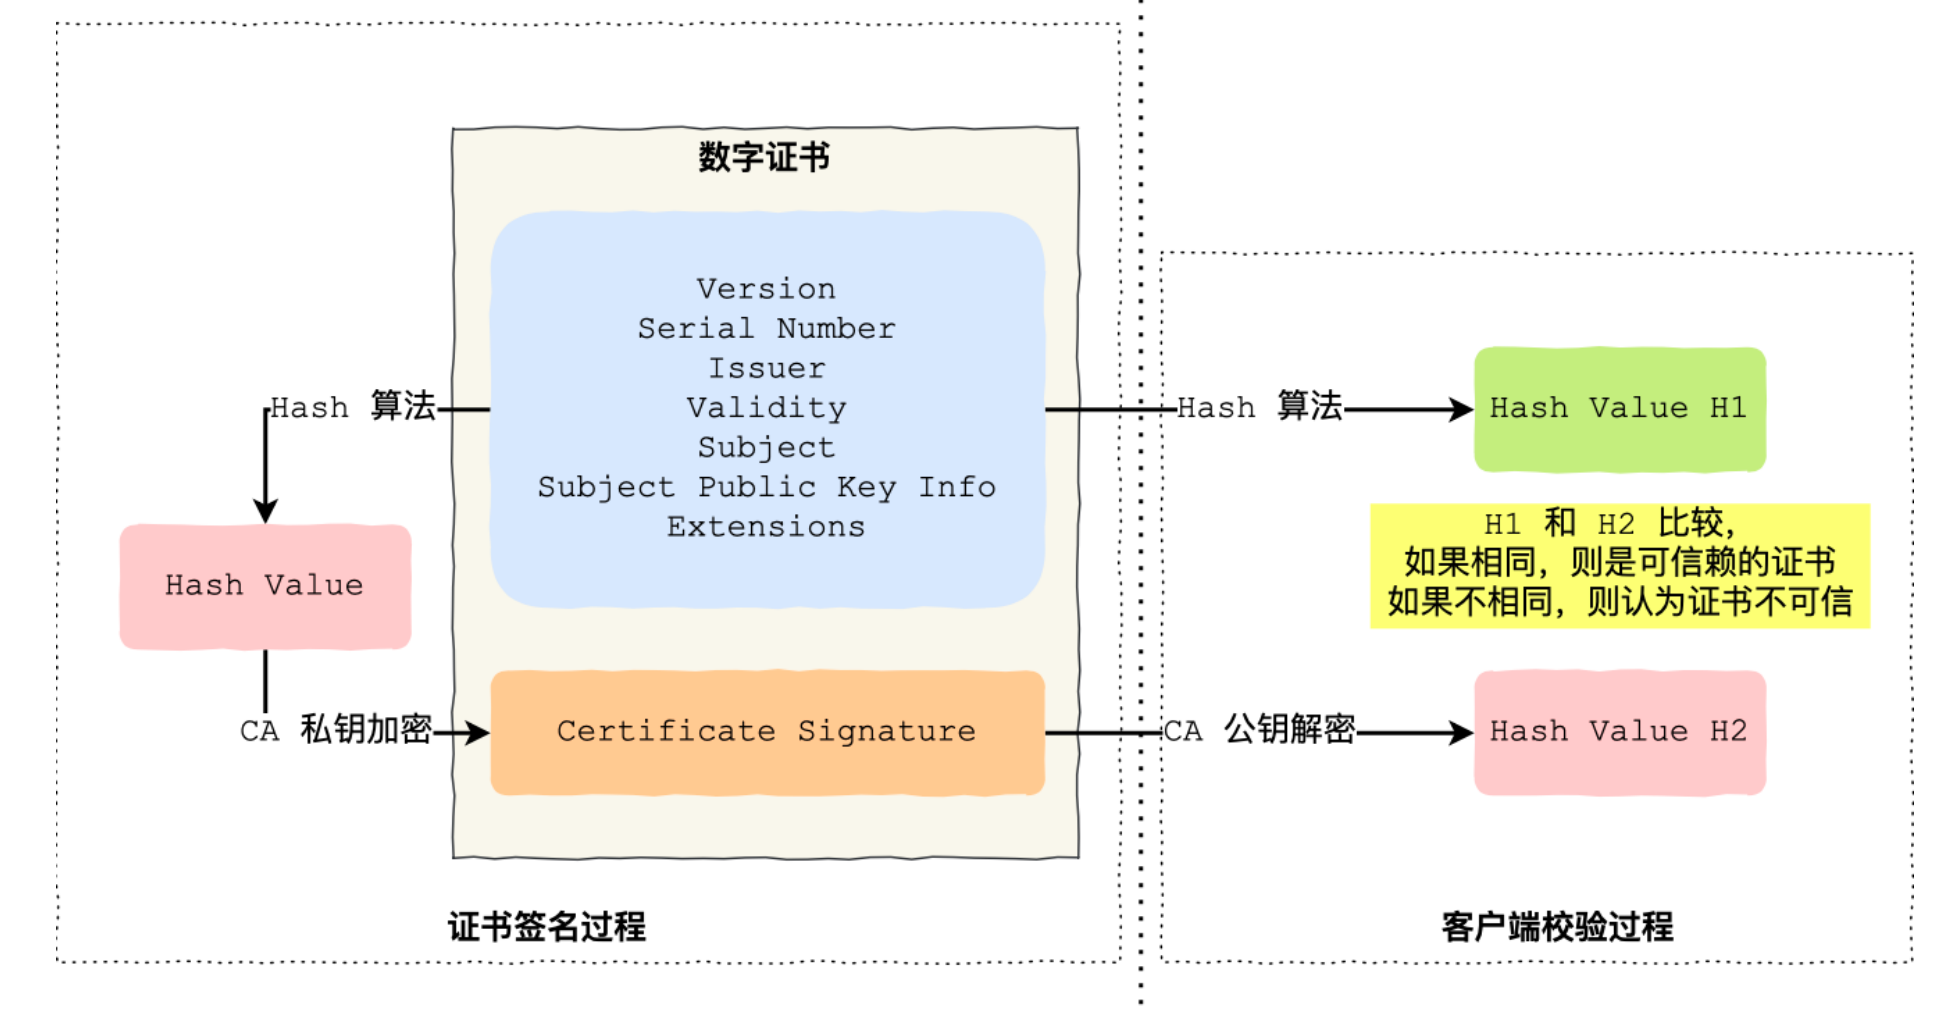
\includegraphics[width=1.0\textwidth]{./Chapter3/q27_1.png}
\caption{证书签名过程和客户端校验过程}
\label{fig27_1}
\end{figure}

CA 签发证书的过程,如上图\ref{fig27_1} 左边部分:
\begin{enumerate}
	\item 首先 CA 会把持有者的公钥、用途、颁发者、有效时间等信息打成一个包,然后对这些信息进行 Hash 计算,得到一个 Hash 值;
	\item 然后 CA 会使用自己的私钥将该 Hash 值加密,生成 Certificate Signature,也就是 CA 对证书做了签名;
	\item 最后将 Certificate Signature 添加在文件证书上,形成数字证书;
\end{enumerate}

客户端校验服务端的数字证书的过程,如上图\ref{fig27_1} 右边部分:
\begin{enumerate}
	\item 首先客户端会使用同样的 Hash 算法获取该证书的 Hash 值 H1;
	\item 通常浏览器和操作系统中集成了 CA 的公钥信息,浏览器收到证书后可以使用 CA 的公钥解密 Certificate;
	\item Signature 内容,得到一个 Hash 值 H2 ;
	\item 最后比较 H1 和 H2,如果值相同,则为可信赖的证书,否则则认为证书不可信。
\end{enumerate}
假如在 HTTPS 的通信过程中,中间人篡改了证书原文,由于他没有 CA 机构的私钥,所以 CA 公钥解密的内容就不一致。

\end{solution}


%------------- 问题28 -------------------
\begin{custom}{问题28}
如何理解 HTTP 协议是无状态的?
\end{custom}
\begin{solution}
这个无状态的的状态值的是什么?是客户端的状态,所以字面意思,就是HTTP协议中服务端不会保存客户端的任何信息。

比如当浏览器第一次发送请求给服务器时,服务器响应了;如果同个浏览器发起第二次请求给服务器时,它还是会响应,但是呢,服务器不知道你就是刚才的那个浏览器。

那有什么办法记录状态呢?

主要有两个办法,Session 和 Cookie。
\end{solution}

%------------- 问题29 -------------------
\begin{custom}{问题29}
说说Session 和 Cookie 有什么联系和区别?
\end{custom}
\begin{solution}
先来看看什么是 Session 和 Cookie :

\begin{itemize}
	\item Cookie 是保存在客户端的一小块文本串的数据。客户端向服务器发起请求时,服务端会向客户端发送一个 Cookie,客户端就把 Cookie 保存起来。在客户端下次向同一服务器再发起请求时,Cookie 被携带发送到服务器。服务端可以根据这个 Cookie 判断用户的身份和状态。
	\item Session 指的就是服务器和客户端一次会话的过程。它是另一种记录客户状态的机制。不同的是cookie 保存在客户端浏览器中,而 session 保存在服务器上。客户端浏览器访问服务器的时候,服务器把客户端信息以某种形式记录在服务器上,这就是 session。客户端浏览器再次访问时只需要从该 session 中查找用户的状态。
\end{itemize}

\begin{figure}[htbp]
\centering
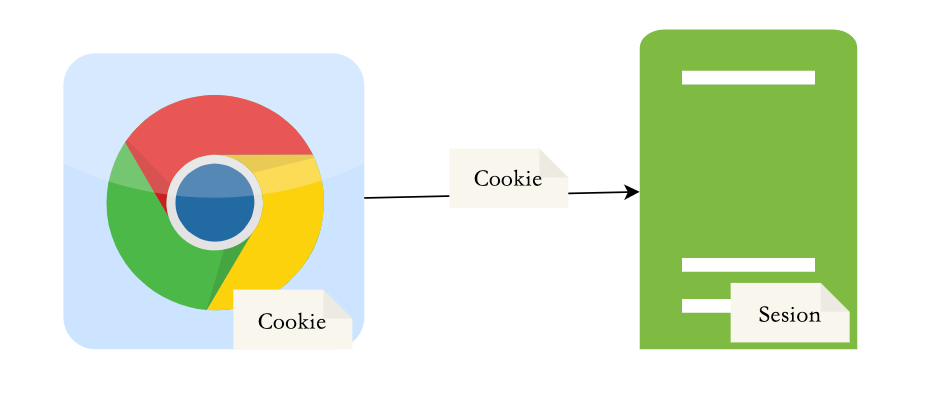
\includegraphics[width=0.7\textwidth]{./Chapter3/q29_1.png}
\caption{cookie 和 session}
\label{fig29_1}
\end{figure}

\begin{note} \textbf{Session 和 Cookie 到底有什么不同呢?} \end{note}
\begin{itemize}
	\item 存储位置不一样,Cookie 保存在客户端,Session 保存在服务器端。
	\item 存储数据类型不一样,Cookie 只能保存ASCII,Session可以存任意数据类型,一般情况下我们可以在 Session 中保持一些常用变量信息,比如说 UserId 等。
	\item 有效期不同,Cookie 可设置为长时间保持,比如我们经常使用的默认登录功能,Session 一般有效时间较短,客户端关闭或者 Session 超时都会失效。
	\item 隐私策略不同,Cookie 存储在客户端,比较容易遭到不法获取,早期有人将用户的登录名和密码存储在 Cookie 中导致信息被窃取;Session 存储在服务端,安全性相对 Cookie 要好一些。
	\item 存储大小不同, 单个 Cookie 保存的数据不能超过 4K,Session可存储数据远高于 Cookie。
\end{itemize}

\begin{note} \textbf{Session 和 Cookie 有什么关联呢?} \end{note}
\begin{figure}[htbp]
\centering
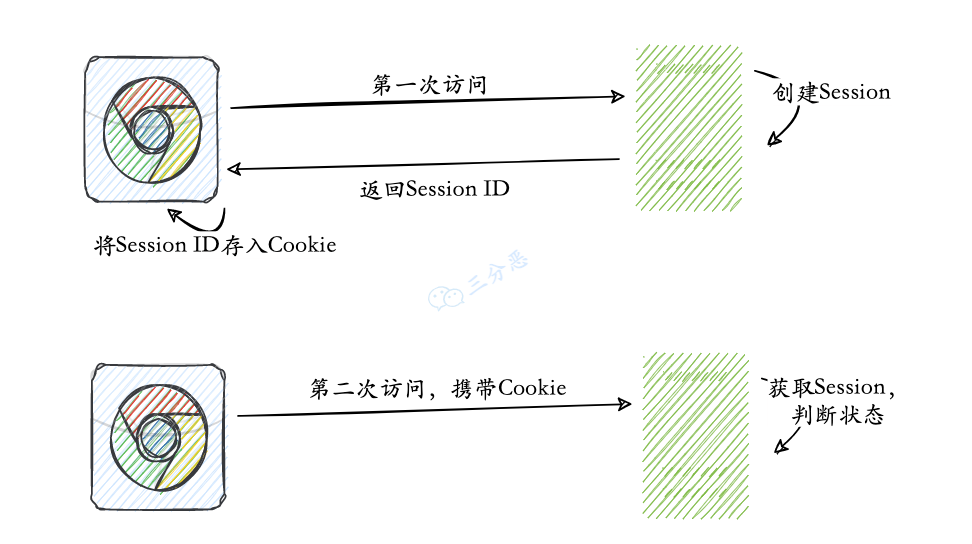
\includegraphics[width=0.7\textwidth]{./Chapter3/q29_2.png}
\caption{cookie 和 session 的创建}
\label{fig29_2}
\end{figure}
\begin{itemize}
	\item 用户第一次请求服务器时,服务器根据用户提交的信息,创建对应的 Session,请求返回时将此 Session 的唯一标识信息 SessionID 返回给浏览器,浏览器接收到服务器返回的 SessionID 信息后,会将此信息存入 Cookie 中,同时 Cookie 记录此 SessionID 是属于哪个域名。
	\item 当用户第二次访问服务器时,请求会自动判断此域名下是否存在 Cookie 信息,如果存在,则自动将 Cookie 信息也发送给服务端,服务端会从 Cookie 中获取 SessionID,再根据 SessionID 查找对应的 Session 信息,如果没有找到,说明用户没有登录或者登录失效,如果找到 Session 证明用户已经登录可执行后面操作。
\end{itemize}

\begin{note} \textbf{分布式环境下Session怎么处理呢?} \end{note}
\begin{figure}[htbp]
\centering
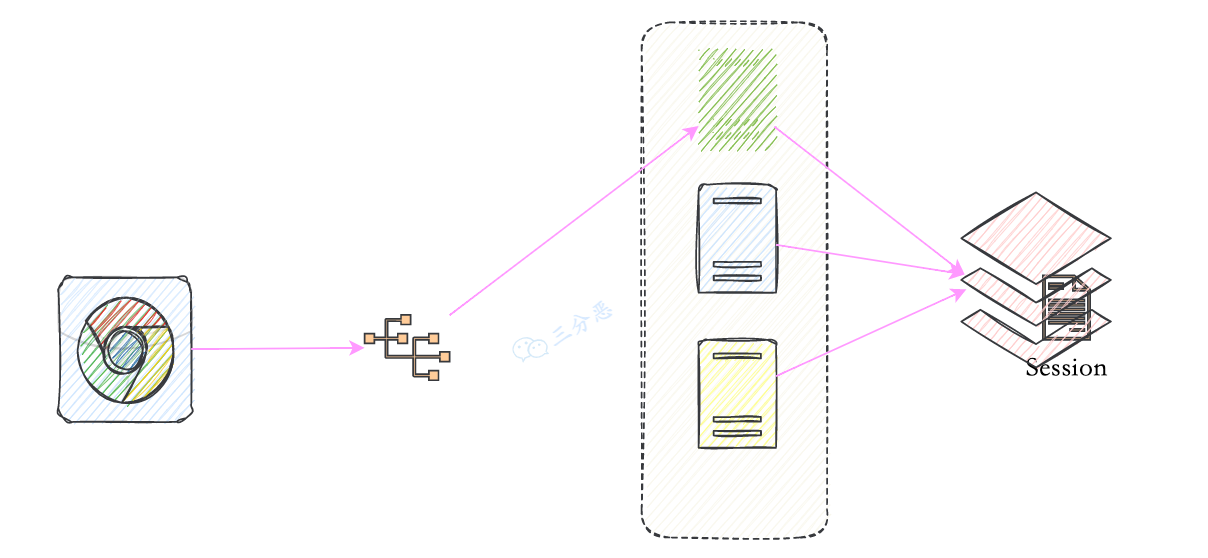
\includegraphics[width=0.5\textwidth]{./Chapter3/q29_3.png}
\caption{Redis 分布时存储 Session}
\label{fig29_3}
\end{figure}

分布式环境下,客户端请求经过负载均衡,可能会分配到不同的服务器上,假如一个用户的请求两次没有落到同一台服务器上,那么在新的服务器上就没有记录用户状态的 Session。

这时候怎么办呢?

可以使用 Redis 等分布式缓存来存储 Session,在多台服务器之间共享。
\begin{note} \textbf{客户端无法使用Cookie怎么办?} \end{note}

有可能客户端无法使用 Cookie,比如浏览器禁用 Cookie,或者客户端是安卓、IOS 等等。

这时候怎么办?SessionID 怎么存?怎么传给服务端呢?

首先是 SessionID 的存储,可以使用客户端的本地存储,比如浏览器的 sessionStorage。

接下来怎么传呢?
\begin{itemize}
	\item 拼接到 URL 里:直接把 SessionID 作为 URL 的请求参数
	\item 放到请求头里:把 SessionID 放到请求的 Header 里,比较常用。
\end{itemize}

\end{solution}


\chapter{传输层对应问题}
\section{TCP 传输协议}

%------------- 问题30 -------------------
\begin{custom}{问题30}
TCP是如何实现差错控制的?
\end{custom}
\begin{solution}
xxxxxxxxxxxxxxxxxxxx
\end{solution}

%------------- 问题31 -------------------
\begin{custom}{问题31}
详细说一下 TCP 的三次握手机制
\end{custom}
\begin{solution}
PS:TCP三次握手是最重要的知识点,一定要熟悉到问到即送分。

TCP 提供面向连接的服务,在传送数据前必须建立连接,TCP 连接是通过三次握手建立的。其过程如下图\ref{fig31_1} 所示:
\begin{figure}[htbp]
\centering
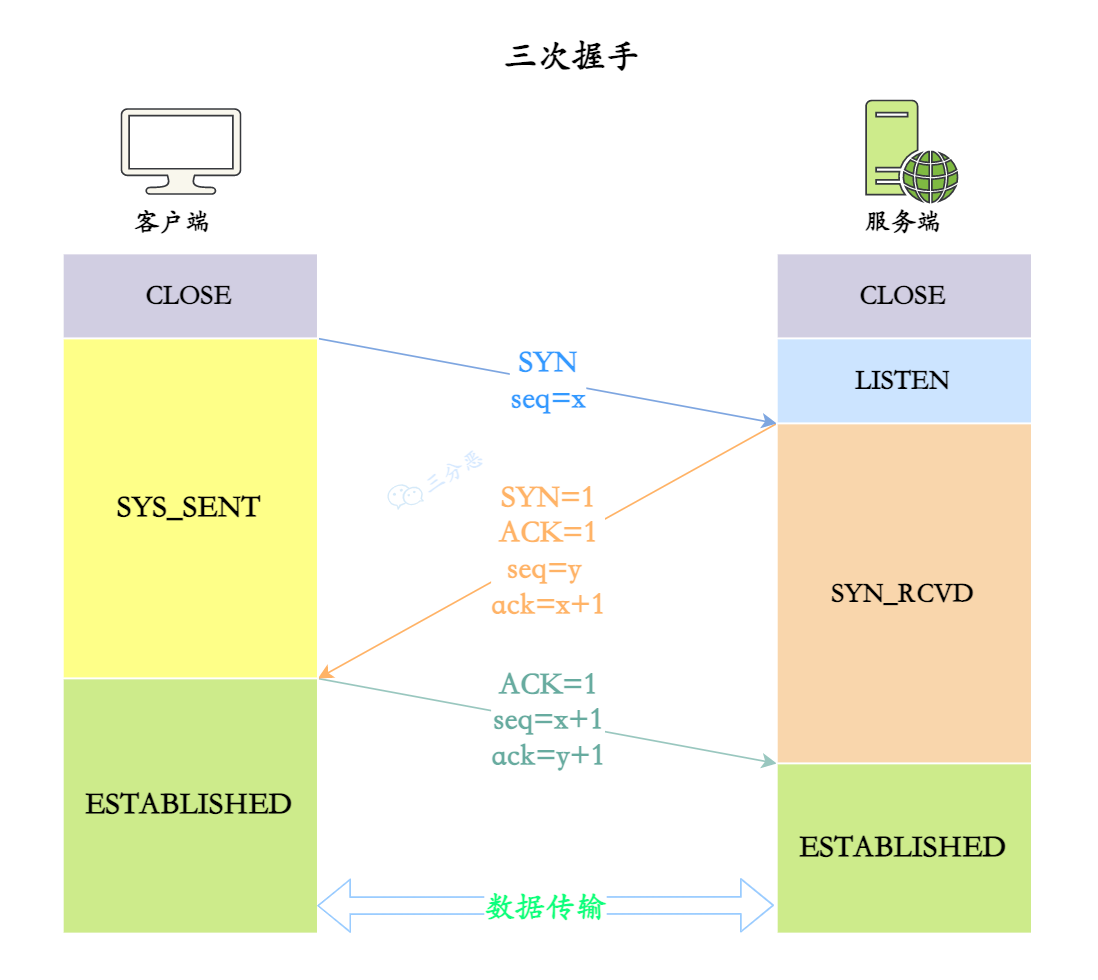
\includegraphics[width=0.7\textwidth]{./Chapter4/q31_1.png}
\caption{TCP 三次握手连接}
\label{fig31_1}
\end{figure}

三次握手的过程:
\begin{enumerate}
	\item 最开始,客户端和服务端都处于 CLOSE 状态,服务端监听客户端的请求,进入 LISTEN 状态
	\item 客户端端发送连接请求,\textbf{第一次握手}(SYN=1, seq=x),发送完毕后,客户端就进入 SYN\_SENT 状态
	\item 服务端确认连接,\textbf{第二次握手}(SYN=1, ACK=1, seq=y, ACKnum=x+1), 发送完毕后,服务器端就进入 SYN\_RCV 状态。
	\item 客户端收到服务端的确认之后,再次向服务端确认,这就是\textbf{第三次握手} (ACK=1,ACKnum=y+1),发送完毕后,客户端进入 ESTABLISHED 状态,当服务器端接收到这个包时,也进入 ESTABLISHED 状态。
\end{enumerate}

TCP三次握手通俗比喻:在二十年前的农村,电话没有普及,手机就更不用说了,所以,通信基本靠吼。老张和老王是邻居,这天老张下地了,结果家里有事,热心的邻居老王赶紧跑到村口,开始叫唤老王。

\begin{enumerate}
	\item 老王:老张唉!我是老王,你能听到吗?
	\item 老张一听,是老王的声音:老王老王,我是老张,我能听到,你能听到吗?
	\item 老王一听,嗯,没错,是老张:老张,我听到了,我有事要跟你说。"你老婆要生了,赶紧回家吧!"
\end{enumerate}  

老张风风火火地赶回家,老婆顺利地生了个带把的大胖小子。握手的故事充满了幸福和美满。
\begin{figure}[htbp]
\centering
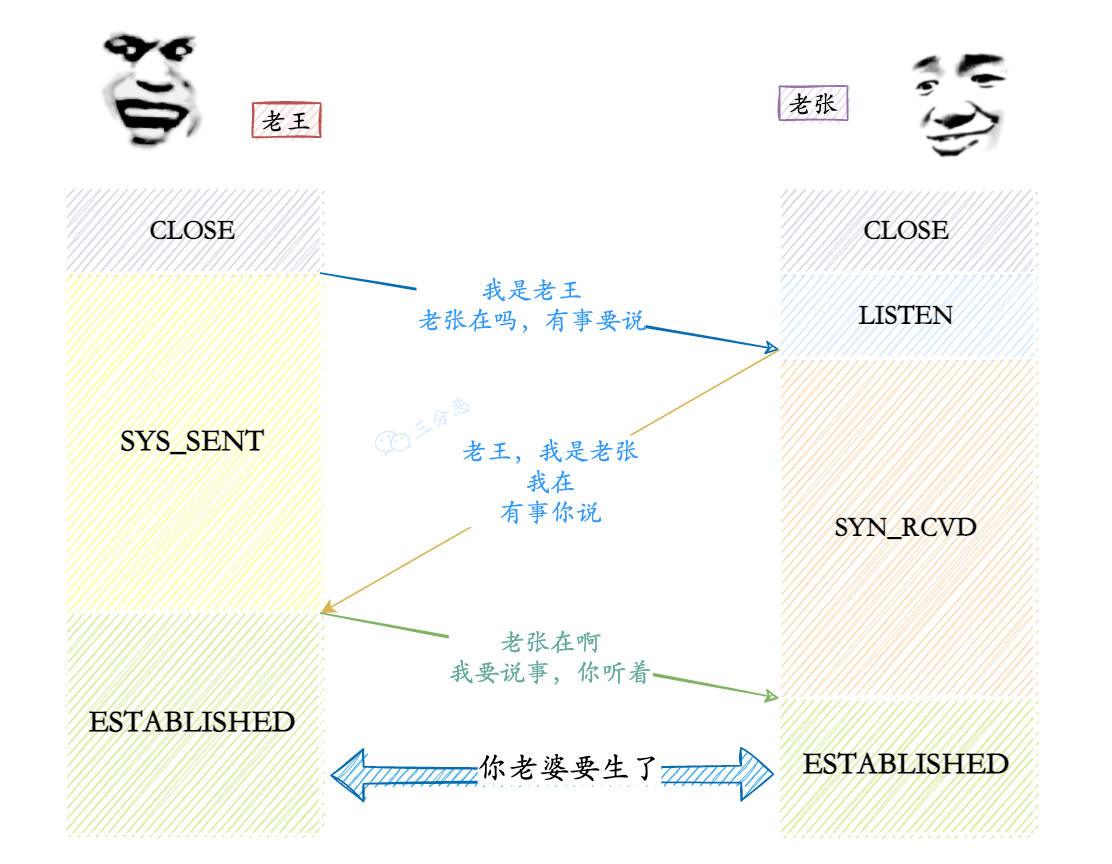
\includegraphics[width=0.7\textwidth]{./Chapter4/q31_2.png}
\caption{三次连接通话}
\label{fig31_2}
\end{figure}
\end{solution}

%--------------------------------------------- 问题32 ------------------------------------
\begin{custom}{问题32}
TCP 握手为什么是三次,为什么不能是两次?不能是四次?
\end{custom}

\begin{solution}
\begin{note} \textbf{为什么不能是两次?} \end{note}
TCP 握手不为两次的目的有 2 个:
\begin{itemize}
	\item 为了防止服务器端开启一些无用的连接增加服务器开销
	\item 防止已失效的连接请求报文段突然又传送到了服务端,因而产生错误。
\end{itemize}

由于网络传输是有延时的(要通过网络光纤和各种中间代理服务器),在传输的过程中,比如客户端发起了 SYN=1 的第一次握手。

如果服务器端就直接创建了这个连接并返回包含 SYN、ACK 和 Seq 等内容的数据包给客户端,这个数据包因为网络传输的原因丢失了,丢失之后客户端就一直没有接收到服务器返回的数据包。

如果没有第三次握手告诉服务器端,客户端能够收得到服务器端传输的数据的话,服务器端是不知道客户端有没有接收到服务器端返回的信息的。

服务端就认为这个连接是可用的,端口就一直开着,等到客户端因超时重新发出请求时,服务器就会重新开启一个端口连接。这样一来,就会有很多无效的连接端口白白地开着,导致资源的浪费,如下图\ref{fig32_1} 所示。
\begin{figure}[htbp]
\centering
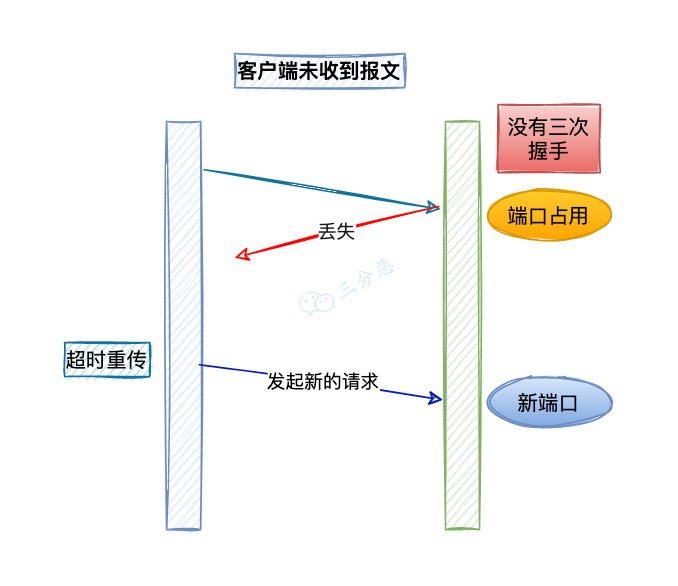
\includegraphics[width=0.7\textwidth]{./Chapter4/q32_1.png}
\caption{无三次握手导致端口占用}
\label{fig32_1}
\end{figure}
还有一种情况是已经失效的客户端发出的请求信息,由于某种原因传输到了服务器端,服务器端以为是客户端发出的有效请求,接收后产生错误,如下图\ref{fig32_2}所示。

\begin{figure}[!h]
\centering
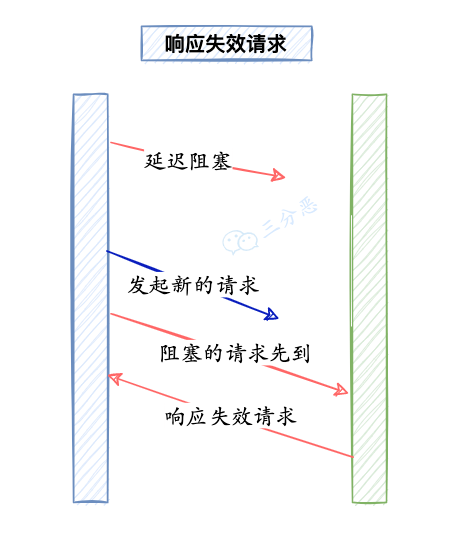
\includegraphics[width=0.4\textwidth]{./Chapter4/q32_2.png}
\caption{响应失效客户端请求}
\label{fig32_2}
\end{figure}

所以我们需要 “第三次握手” 来确认这个过程:通过第三次握手的数据告诉服务端,客户端有没有收到服务器“第二次握手”时传过去的数据,以及这个连接的序号是不是有效的。若发送的这个数据是“收到且没有问题”的信息,接收后服务器就正常建立 TCP 连接,否则建立 TCP 连接失败,服务器关闭连接端口。由此减少服务器开销和接收到失效请求发生的错误。
\newpage
\begin{note} \textbf{为什么不是四次} \end{note}
简单说,就是三次挥手已经足够创建可靠的连接,没有必要再多一次握手导致花费更多的时间建立连接。
\end{solution}

%--------------------------------------------- 问题33 ------------------------------------
\begin{custom}{问题33}
三次握手中每一次没收到报文会发生什么情况?
\end{custom}

\begin{solution}
先将 TCP 三次连接的图放到这里,这个图之前出现过一次,也是最重要的图,将会多次出现。
\begin{figure}[htbp]
\centering
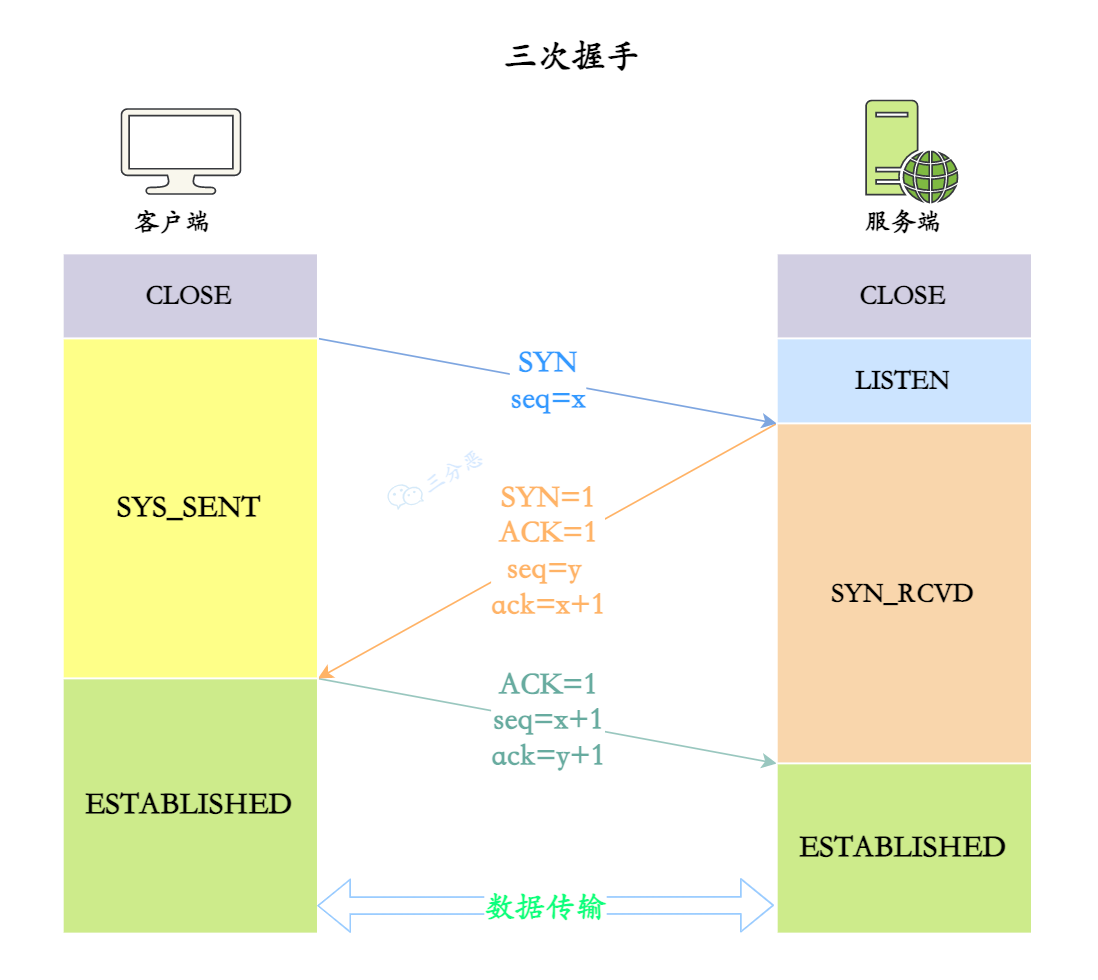
\includegraphics[width=0.7\textwidth]{./Chapter4/q31_1.png}
\caption{TCP 三次握手连接}
\end{figure}
\end{solution}

\begin{note} \textbf{第一次握手服务端未收到 SYN 报文} \end{note}
 服务端不会进行任何的动作,而客户端由于一段时间内没有收到服务端发来的确认报文,等待一段时间后会重新发送 SYN 报文,如果仍然没有回应,会重复这个过程,直到发送次数超过最大重传次数限制,就会返回连接建立失败。

\begin{note} \textbf{第二次握手客户端未收到服务端响应的 ACK 报文} \end{note}
客户端会继续重传,直到次数限制;而服务端此时会阻塞在 accept() 处,等待客户端发送 ACK 报文

\begin{note} \textbf{第三次握手服务端未收到客户端发送过来的 ACK 报文} \end{note}
服务端同样会采用类似客户端的超时重传机制,如果重试次数超过限制,则 accept() 调用返回 -1,服务端建立连接失败;

而此时客户端认为自己已经建立连接成功,因此开始向服务端发送数据,但是服务端的 accept() 系统调用已经返回,此时不在监听状态,因此服务端接收到客户端发送来的数据时会发送 RST 报文给客户端,消除客户端单方面建立连接的状态。


%--------------------------------------------- 问题34 ------------------------------------
\begin{custom}{问题34}
第二次握手传回了 ACK,为什么还要传回 SYN?
\end{custom}
\begin{solution}
ACK 是为了告诉客户端传来的数据已经接收无误。

而传回 SYN 是为了告诉客户端,服务端响应的确实是客户端发送的报文。
\end{solution}

%--------------------------------------------- 问题35 ------------------------------------
\begin{custom}{问题35}
第二次握手传回了 ACK,为什么还要传回 SYN?
\end{custom}
\begin{solution}
第3次握手是可以携带数据的。

此时客户端已经处于 ESTABLISHED 状态。对于客户端来说,它已经建立连接成功,并且确认服务端的接收和发送能力是正常的。

第一次握手不能携带数据是出于安全的考虑,因为如果允许携带数据,攻击者每次在 SYN 报文中携带大量数据,就会导致服务端消耗更多的时间和空间去处理这些报文,会造成 CPU 和内存的消耗。
\end{solution}

%--------------------------------------------- 问题36 ------------------------------------
\begin{custom}{问题36}
说说半连接队列和 SYN Flood 攻击的关系?
\end{custom}
\begin{solution}
\begin{note} \textbf{什么是半连接队列} \end{note}
TCP 进入三次握手前,服务端会从 CLOSED 状态变为 LISTEN 状态, 同时在内部创建了两个队列:半连接队列(SYN 队列)和全连接队列(ACCEPT 队列)。
\begin{figure}[htbp]
\centering
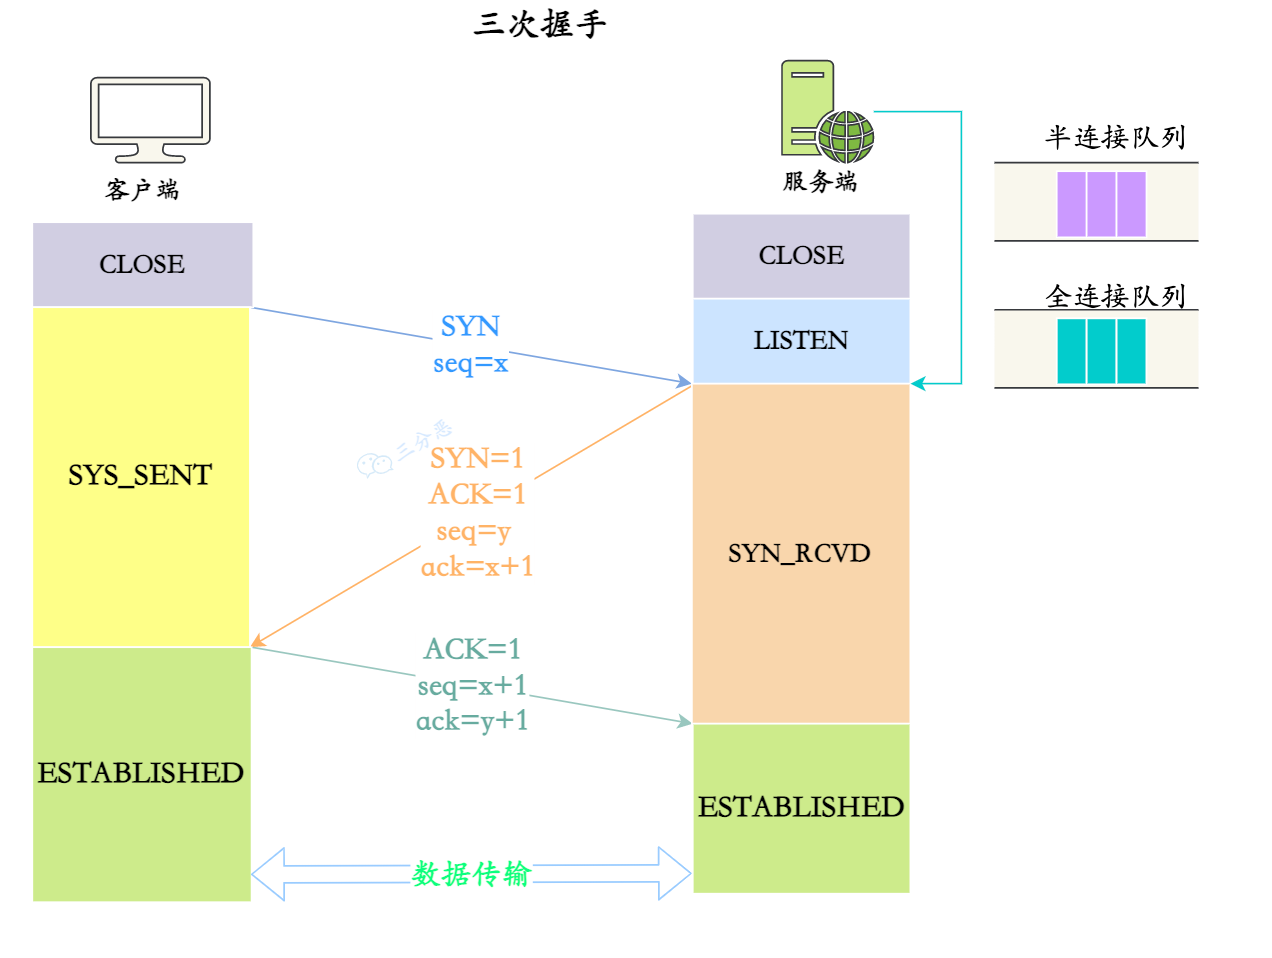
\includegraphics[width=0.7\textwidth]{./Chapter4/q36_1.png}
\caption{TCP 三次握手中创建的队列}
\label{fig36_1}
\end{figure}


顾名思义,半连接队列存放的是三次握手未完成的连接,全连接队列存放的是完成三次握手的连接。
\begin{itemize}
	\item 在 TCP 三次握手的第一次握手时,客户端发送 SYN 到服务端,服务端收到之后,便回复 ACK 和 SYN,状态由 LISTEN 变为 SYN\_RCVD,此时这个连接就被推入了 SYN 队列,即半连接队列。
	\item 在 TCP 三次握手的第三次握手时,当客户端回复 ACK, 服务端接收后,三次握手就完成了。这时连接会等待被具体的应用取走,在被取走之前,它被推入 ACCEPT 队列,即全连接队列。
\end{itemize}
\begin{note} \textbf{什么是 SYN 泛洪} \end{note}

SYN Flood 是一种典型的 DDos 攻击,它在短时间内,伪造不存在的 IP 地址, 向服务器发送大量 SYN 报文。当服务器回复 SYN+ACK 报文后,不会收到 ACK 回应报文,那么 SYN 队列里的连接就不会出队,久而久之就会占满服务端的 SYN 接收队列(半连接队列),使得服务器不能为正常用户服务,如下图\ref{fig36_2} 所示。
\begin{figure}[htbp]
\centering
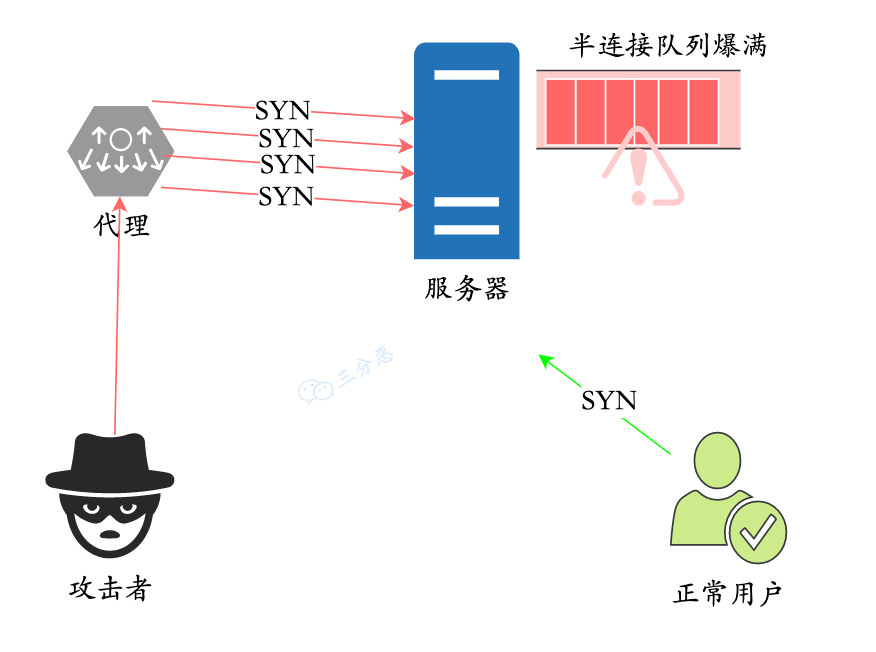
\includegraphics[width=0.7\textwidth]{./Chapter4/q36_2.png}
\caption{SYN 泛洪攻击}
\label{fig36_2}
\end{figure}


\begin{note} \textbf{SYN 泛洪应对方案} \end{note}
主要有 syn cookie 和 SYN Proxy 防火墙等。
\begin{itemize}
	\item syn cookie:在收到 SYN 包后,服务器根据一定的方法,以数据包的源地址、端口等信息为参数计算出一个 cookie 值作为自己的 SYNACK 包的序列号,回复 SYN+ACK 后,服务器并不立即分配资源进行处理,等收到发送方的 ACK 包后,重新根据数据包的源地址、端口计算该包中的确认序列号是否正确,如果正确则建立连接,否则丢弃该包。
	\item SYN Proxy 防火墙:服务器防火墙会对收到的每一个 SYN 报文进行代理和回应,并保持半连接。等发送方将 ACK 包返回后,再重新构造 SYN 包发到服务器,建立真正的 TCP 连接。
\end{itemize}
\end{solution}

%--------------------------------------------- 问题37 ------------------------------------
\begin{custom}{问题37}
说说 TCP 四次挥手的过程?
\end{custom}
\begin{solution}
PS:问完三次握手,常常也会顺道问问四次挥手,所以也是必须掌握知识点。TCP 四次挥手过程如下图\ref{fig37_1} 所示:

\begin{figure}[htbp]
\centering
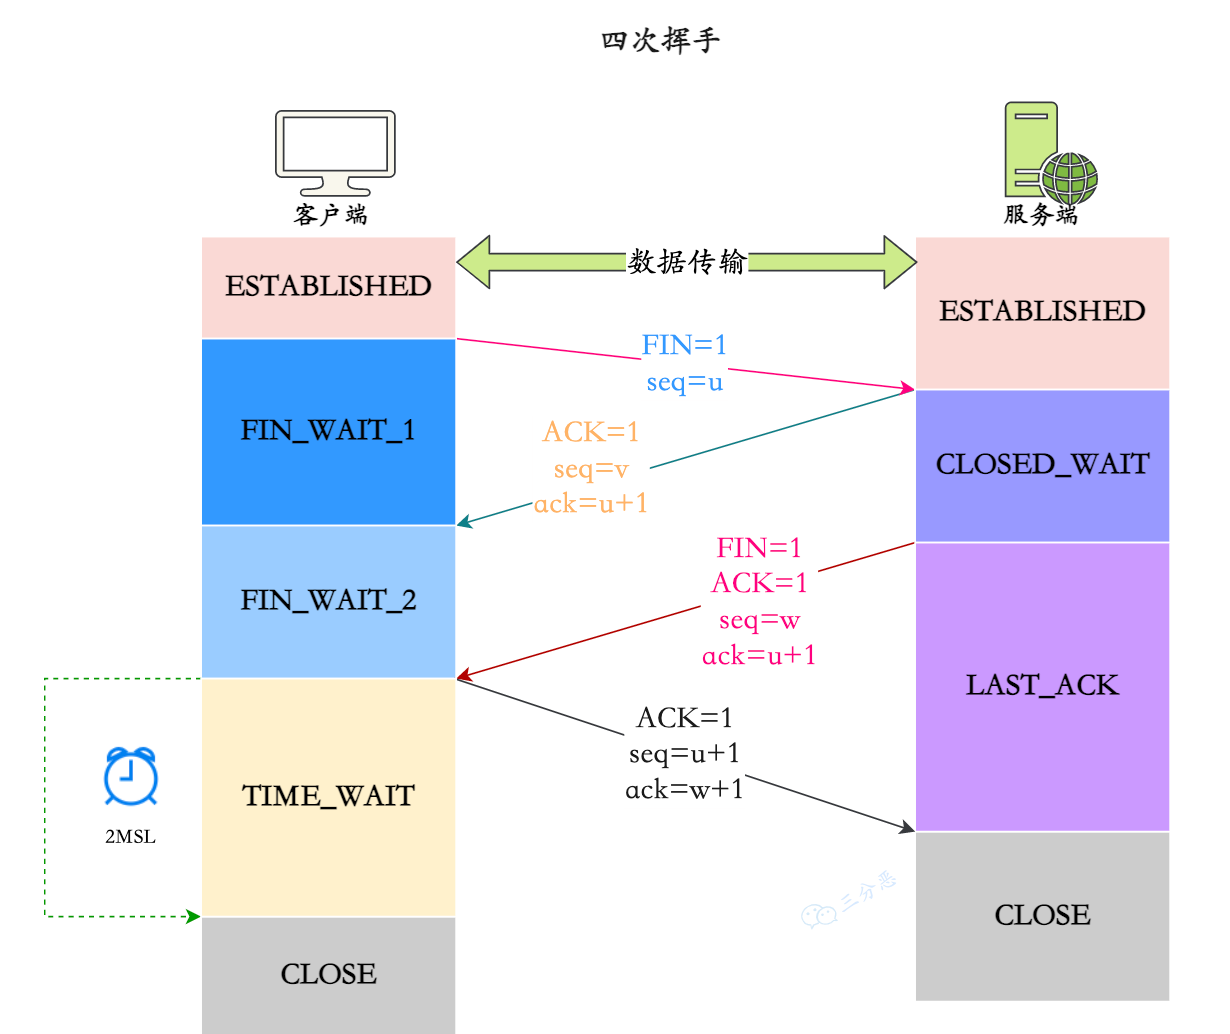
\includegraphics[width=0.7\textwidth]{./Chapter4/q37_1.png}
\caption{TCP 四次回收}
\label{fig37_1}
\end{figure}


TCP 四次挥手过程:数据传输结束之后,通信双方都可以主动发起断开连接请求,这里假定客户端发起

\begin{enumerate}
	\item 客户端发送释放资源连接报文,第一次挥手 (FIN=1,seq=u),发送完毕后,客户端进入 FIN\_WAIT\_1 状态。
	\item 服务端发送确认报文,第二次挥手 (ACK=1,ack=u+1,seq=v),发送完毕后,服务器端进入 CLOSE\_WAIT 状态,客户端接收到这个确认包之后,进入 FIN\_WAIT\_2 状态。
	\item 服务端发送释放连接报文,第三次挥手 (FIN=1, ACK1, seq=w, ack=u+1),发送完毕后,服务器端进入 LAST\_ACK 状态,等待来自客户端的最后一个 ACK。
	\item 客户端发送确认报文,第四次挥手 (ACK=1, seq=u+1, ack=w+1),客户端接收到来自服务器端的关闭请求,发送一个确认包,并进入 TIME\_WAIT 状态,等待了某个固定时间(两个最大段生命周期,2MSL,2 Maximum Segment Lifetime)之后,没有收到服务器端的 ACK ,认为服务器端已经正常关闭连接,于是自己也关闭连接,进入 CLOSED 状态。服务器端接收到这个确认包之后,关闭连接,进入 CLOSED 状态。
\end{enumerate}

大白话说四次挥手:

假如单身狗博主有一个女朋友—由于博主上班九九六,下班肝博客,导致没有时间陪女朋友,女朋友忍无可忍。

\begin{enumerate}
	\item 女朋友:狗男人,最近你都不理我,你是不是不爱我了?你是不是外面有别的狗子了?我要和你分手?
	\item 沙雕博主一愣,怒火攻心:分手就分手,不陪你闹了,等我把东西收拾收拾。
\end{enumerate}
沙雕博主小心翼翼地装起了自己的青轴机械键盘。
\begin{enumerate}
	\item 哼,蠢女人,我已经收拾完了,我先滚为敬,再见!
	\item 女朋友:滚,滚的远远的,越远越好,我一辈子都不想再见到你。
\end{enumerate}
整个挥手过程如下图\ref{fig37_2} 所示,挥手的故事总充满了悲伤和遗憾!
\begin{figure}[htbp]
\centering
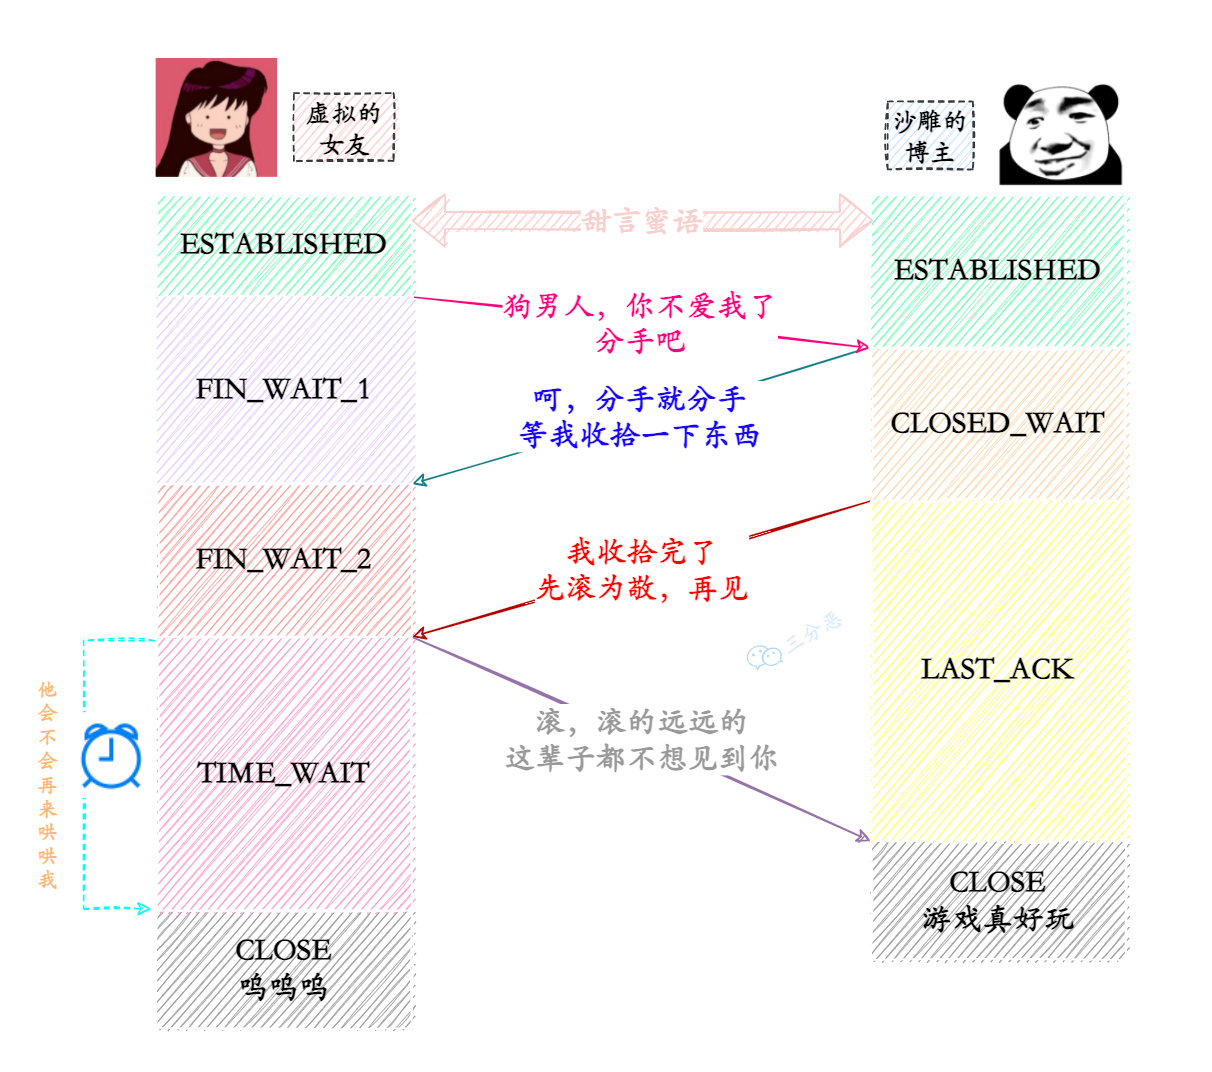
\includegraphics[width=0.7\textwidth]{./Chapter4/q37_2.png}
\caption{大白话四次挥手}
\label{fig37_2}
\end{figure}

\end{solution}


%--------------------------------------------- 问题38 ------------------------------------
\begin{custom}{问题38}
TCP 挥手为什么需要四次呢?
\end{custom}
\begin{solution}
再来回顾下四次挥手双方发 FIN 包的过程,就能理解为什么需要四次了。

\begin{itemize}
	\item 关闭连接时,客户端向服务端发送 FIN 时,仅仅表示客户端不再发送数据了但是还能接收数据。
	\item 服务端收到客户端的 FIN 报文时,先回一个 ACK 应答报文,而服务端可能还有数据需要处理和发送,等服务端不再发送数据时,才发送 FIN 报文给客户端来表示同意现在关闭连接。
\end{itemize}
从上面过程可知,服务端通常需要等待完成数据的发送和处理,所以服务端的 ACK 和 FIN 一般都会分开发送,从而比三次握手导致多了一次。
\end{solution}

%--------------------------------------------- 问题39 ------------------------------------
\begin{custom}{问题39}
TCP 四次挥手过程中,为什么需要等待 2MSL, 才进入 CLOSED 关闭状态?
\end{custom}
\begin{solution}
\begin{note} \textbf{为什么需要等待} \end{note}

TCP 最后挥手需要等待的原因主要有两点:
\begin{enumerate}
	\item 为了保证客户端发送的最后一个 ACK 报文段能够到达服务端。这个 ACK 报文段有可能丢失,因而使处在 LAST-ACK 状态的服务端就收不到对已发送的 FIN + ACK 报文段的确认。服务端会超时重传这个 FIN+ACK 报文段,而客户端就能在 2MSL 时间内( 超时 + 1MSL 传输)收到这个重传的 FIN+ACK 报文段。接着客户端重传一次确认,重新启动 2MSL 计时器。最后,客户端和服务器都正常进入到 CLOSED 状态。

	\item 防止已失效的连接请求报文段出现在本连接中。客户端在发送完最后一个 ACK 报文段后,再经过时间 2MSL,就可以使本连接持续的时间内所产生的所有报文段都从网络中消失。这样就可以使下一个连接中不会出现这种旧的连接请求报文段。
\end{enumerate}
\begin{note} \textbf{为什么等待的时间是 2MSL} \end{note}

MSL 是 Maximum Segment Lifetime,报文最大生存时间,它是任何报文在网络上存在的最长时间,超过这个时间报文将被丢弃。

TIME\_WAIT 等待 2 倍的 MSL,比较合理的解释是: 网络中可能存在来自发送方的数据包,当这些发送方的数据包被接收方处理后又会向对方发送响应,所以一来一回需要等待 2 倍的时间。
\begin{figure}[htbp]
\centering
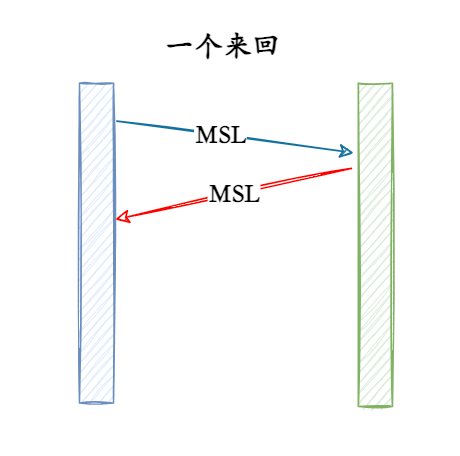
\includegraphics[width=0.4\textwidth]{./Chapter4/q39_1.png}
\caption{TIME\_WAIT 是 2MSL}
\label{fig39_1}
\end{figure}

比如如果被动关闭方没有收到断开连接的最后的 ACK 报文,就会触发超时重发 Fin 报文,另一方接收到 FIN 后,会重发 ACK 给被动关闭方, 一来一去正好 2 个 MSL。
\end{solution}


%--------------------------------------------- 问题40 ------------------------------------
\begin{custom}{问题40}
保活计时器有什么用?
\end{custom}
\begin{solution}
除时间等待计时器外,TCP 还有一个保活计时器(keepalive timer)。

设想这样的场景:客户已主动与服务器建立了 TCP 连接。但后来客户端的主机突然发生故障。显然,服务器以后就不能再收到客户端发来的数据。因此,应当有措施使服务器不要再白白等待下去。这就需要使用保活计时器了。

服务器每收到一次客户端的数据,就重新设置保活计时器,时间的设置通常是两个小时。若两个小时都没有收到客户端的数据,服务端就发送一个探测报文段,以后则每隔 75 秒钟发送一次。若连续发送 10 个探测报文段后仍然无客户端的响应,服务端就认为客户端出了故障,接着就关闭这个连接。
\end{solution}

%--------------------------------------------- 问题41 ------------------------------------
\begin{custom}{问题41}
CLOSE-WAIT 和 TIME-WAIT 的状态和意义?
\end{custom}

\begin{solution}
这次同样也再把四次挥手的图拿出来
\begin{figure}[htbp]
\centering
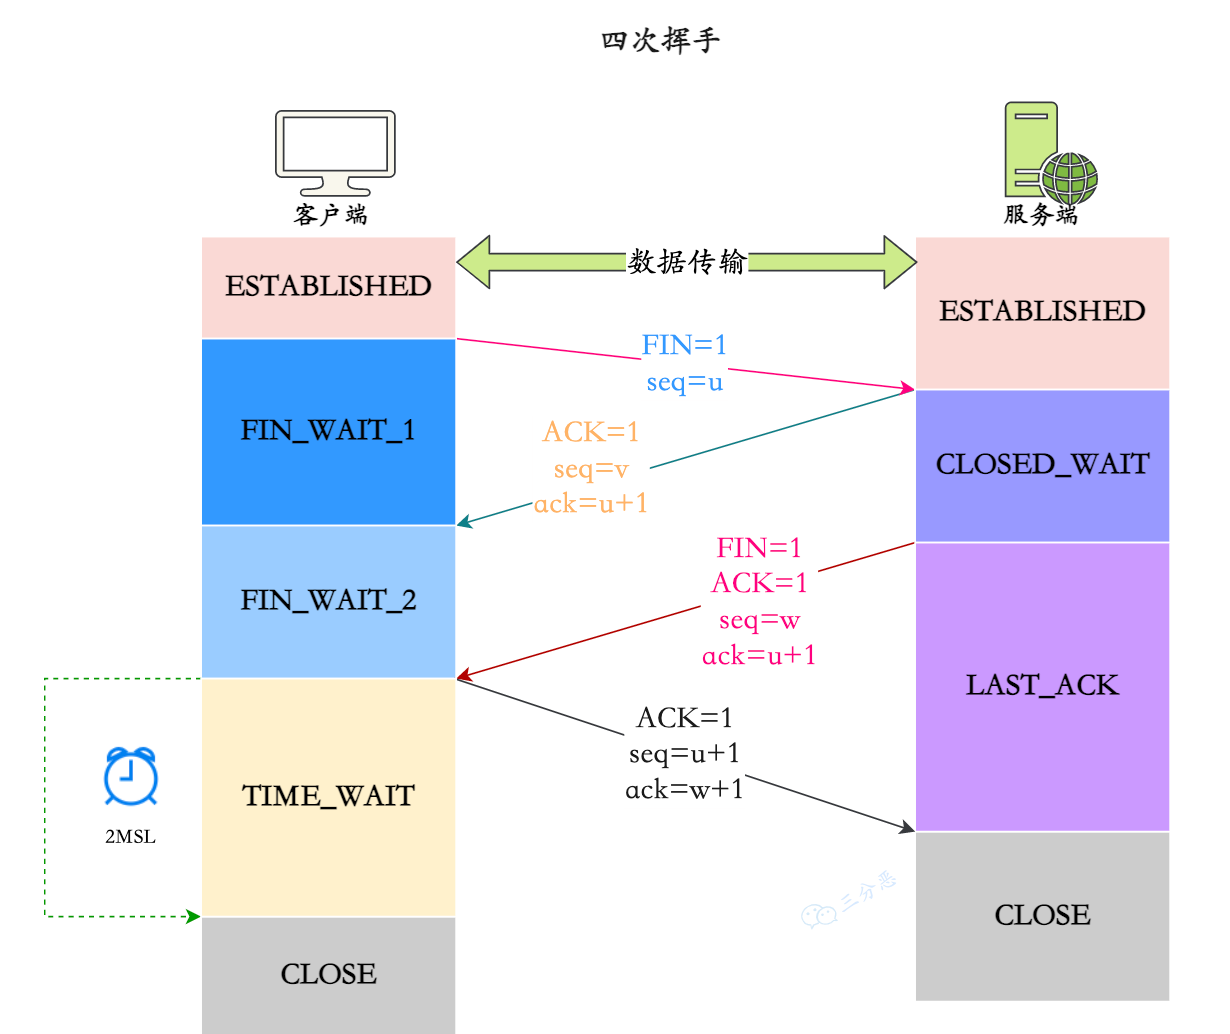
\includegraphics[width=0.55\textwidth]{./Chapter4/q41_1.png}
\caption{TCP 四次挥手}
\end{figure}

\begin{note} \textbf{CLOSED\_WAIT 有什么意义} \end{note}

服务端收到客户端关闭连接的请求并确认之后,就会进入 CLOSE\_WAIT 状态。此时服务端可能还有一些数据没有传输完成,因此不能立即关闭连接,而 CLOSE\_WAIT 状态就是为了保证服务端在关闭连接之前将待发送的数据处理完。
\begin{note} \textbf{TIME\_WAIT 有什么意义} \end{note}

TIME-WAIT状态发生在第四次挥手,当客户端向服务端发送ACK确认报文后进入TIME-WAIT状态。

它存在的意义主要是两个:
\begin{figure}[htbp]
\centering
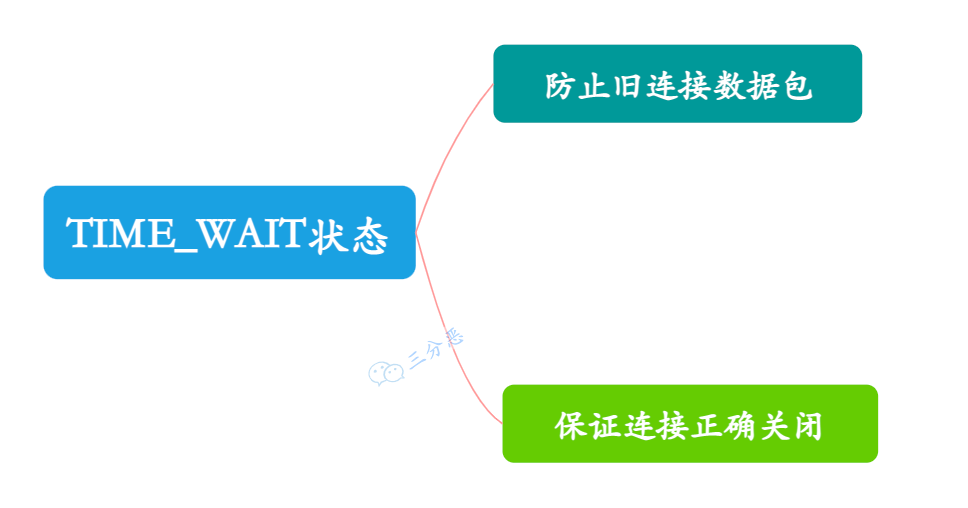
\includegraphics[width=0.65\textwidth]{./Chapter4/q41_2.png}
\caption{TIME\_WAIT 的作用}
\end{figure}

\begin{itemize}
	\item \textbf{防⽌旧连接的数据包。}如果客户端收到服务端的FIN报文之后立即关闭连接,但是此时服务端对应的端口并没有关闭,如果客户端在相同端口建立新的连接,可能会导致新连接收到旧连接残留的数据包,导致不可预料的异常发生。
	\item \textbf{保证连接正确关闭。}假设客户端最后一次发送的ACK包在传输的时候丢失了,由于TCP协议的超时重传机制,服务端将重发FIN报文,如果客户端没有维持TIME-WAIT状态而直接关闭的话,当收到服务端重新发送的FIN包时,客户端就会使用RST包来响应服务端,导致服务端以为有错误发生,然而实际关闭连接过程是正常的。
\end{itemize}

\end{solution}

%--------------------------------------------- 问题42 ------------------------------------
\begin{custom}{问题42}
TIME\_WAIT 状态过多会导致什么问题?怎么解决?
\end{custom}
\begin{solution}
\begin{note} \textbf{TIME\_WAIT 状态过多有什么问题?} \end{note}
(谁先发起断开请求,谁有处于 TIME\_WAIT 状态的 TCP)

如果服务器有处于 TIME\_WAIT 状态的 TCP,则说明是由服务器方主动发起的断开请求。过多的 TIME\_WAIT 状态主要的危害有两种:
\begin{itemize}
	\item 第一是内存资源占用;
	\item 第二是对端口资源的占用,一个 TCP 连接至少消耗一个本地端口;
\end{itemize}
\begin{note} \textbf{TIME\_WAIT 状态过多有什么问题?} \end{note}
\begin{itemize}
	\item 服务器可以设置 SO\_REUSEADDR 套接字来通知内核,如果端口被占用,但是 TCP 连接位于TIME\_WAIT 状态时可以重用端口。
	\item 还可以使用长连接的方式来减少 TCP 的连接和断开,在长连接的业务里往往不需要考虑TIME\_WAIT 状态。
\end{itemize}
\end{solution}

%--------------------------------------------- 问题43 ------------------------------------
\begin{custom}{问题43}
说说 TCP 报文首部的格式?
\end{custom}
\begin{solution}
看一下 TCP 报文首部的格式,如下图\ref{fig43_1} 所示:
\begin{figure}[htbp]
\centering
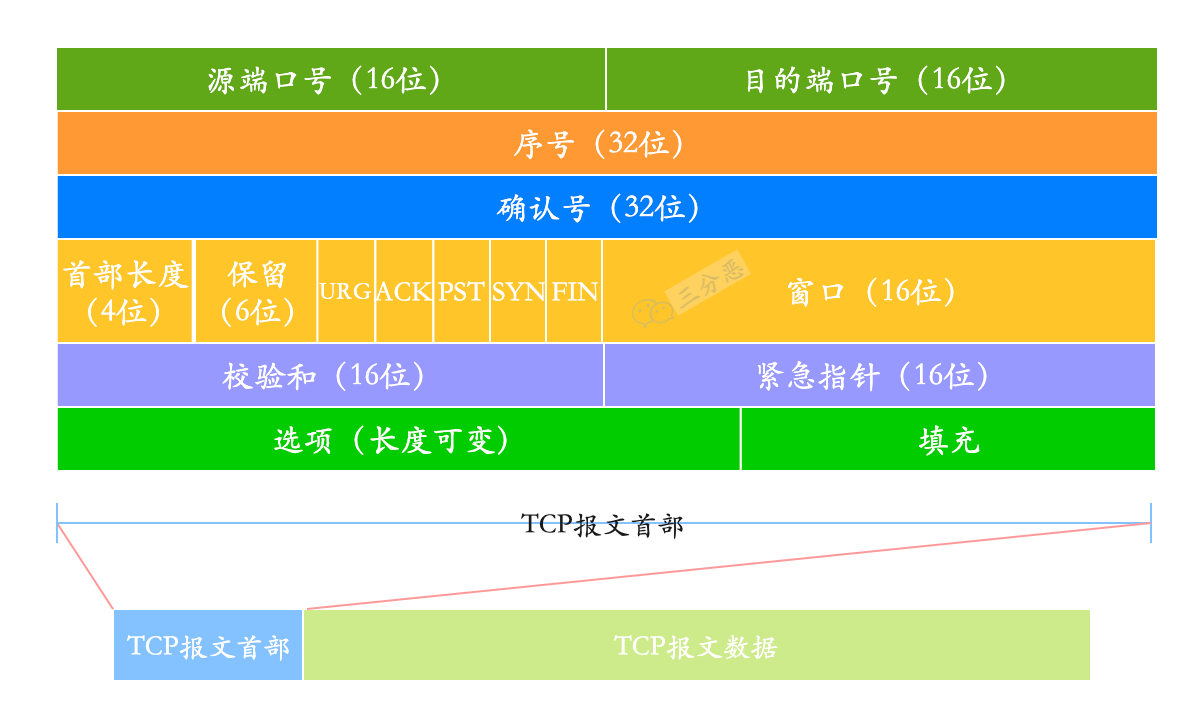
\includegraphics[width=0.9\textwidth]{./Chapter4/q43_1.png}
\caption{TCP 报文首部}
\label{fig43_1}
\end{figure}
\begin{itemize}
	\item \textbf{16 位端口号}:源端口号,主机该报文段是来自哪里;目标端口号,要传给哪个上层协议或应用程序
	\item \textbf{32 位序号}:一次 TCP 通信(从 TCP 连接建立到断开)过程中某一个传输方向上的字节流的每个字节的编号。
	\item \textbf{32 位确认号}:用作对另一方发送的 tcp 报文段的响应。其值是收到的 TCP 报文段的序号值加 1。
	\item \textbf{4 位首部长度}:表示 tcp 头部有多少个 32bit 字(4 字节)。因为 4 位最大能标识 15,所以 TCP 头部最长是 60 字节。
	\item \textbf{6 位标志位}:
		\begin{itemize}
			\item URG:紧急指针是否有效
			\item ACk:表示确认号是否有效
			\item PST:缓冲区尚未填满
			\item RST:表示要求对方重新建立连接
			\item SYN:建立连接消息标志接
			\item FIN:表示告知对方本端要关闭连接了
		\end{itemize}
	\item \textbf{16 位窗口大小}:是 TCP 流量控制的一个手段。这里说的窗口,指的是接收通告窗口。它告诉对方本端的 TCP 接收缓冲区还能容纳多少字节的数据,这样对方就可以控制发送数据的速度。
	\item \textbf{16 位校验和}:由发送端填充,接收端对 TCP 报文段执行 CRC 算法以检验 TCP 报文段在传输过程中是否损坏。注意,这个校验不仅包括 TCP 头部,也包括数据部分。这也是 TCP 可靠传输的一个重要保障。
	\item \textbf{16 位紧急指针}:一个正的偏移量。它和序号字段的值相加表示最后一个紧急数据的下一字节的序号。因此,确切地说,这个字段是紧急指针相对当前序号的偏移,不妨称之为紧急偏移。TCP 的紧急指针是发送端向接收端发送紧急数据的方法。
\end{itemize}
\end{solution}

%--------------------------------------------- 问题44 ------------------------------------
\begin{custom}{问题44}
TCP 是如何保证可靠性的?
\end{custom}
\begin{solution}
TCP主要提供了检验和、序列号/确认应答、超时重传、最大消息长度、滑动窗口控制等方法实现了可靠性传输。
\begin{figure}[htbp]
\centering
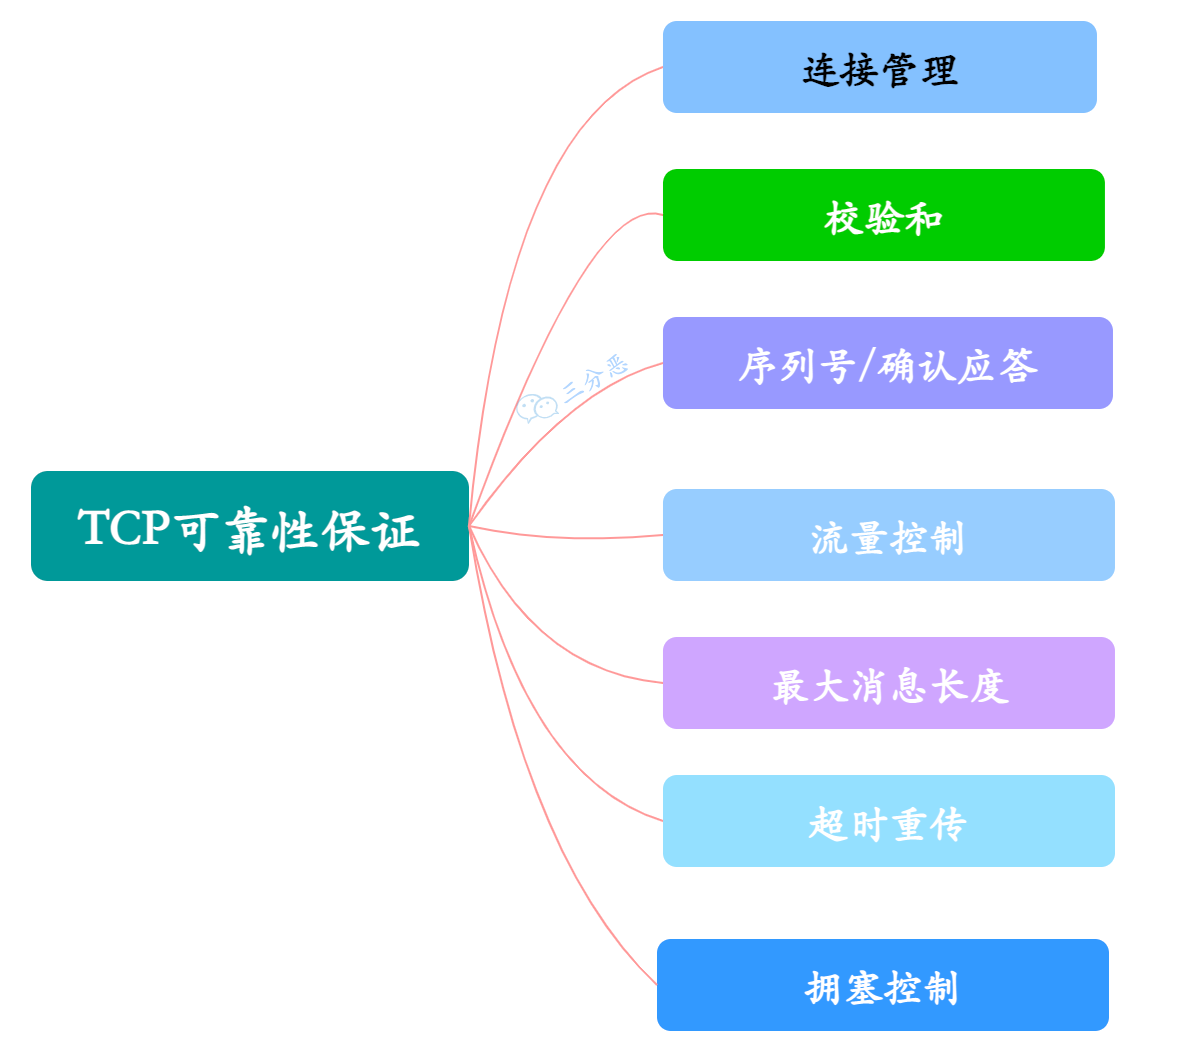
\includegraphics[width=0.7\textwidth]{./Chapter4/q44_1.png}
\caption{TCP 保证可靠性的方法}
\label{fig44_1}
\end{figure}

\begin{note} \textbf{连接管理} \end{note}
TCP 使用三次握手和四次挥手保证可靠地建立连接和释放连接,这里就不用多说了。

\begin{note} \textbf{校验和} \end{note}
TCP 将保持它首部和数据的检验和。这是一个端到端的检验和,目的是检测数据在传输过程中的任何变化。如果接收端的检验和有差错,TCP 将丢弃这个报文段和不确认收到此报文段。
\begin{figure}[htbp]
\centering
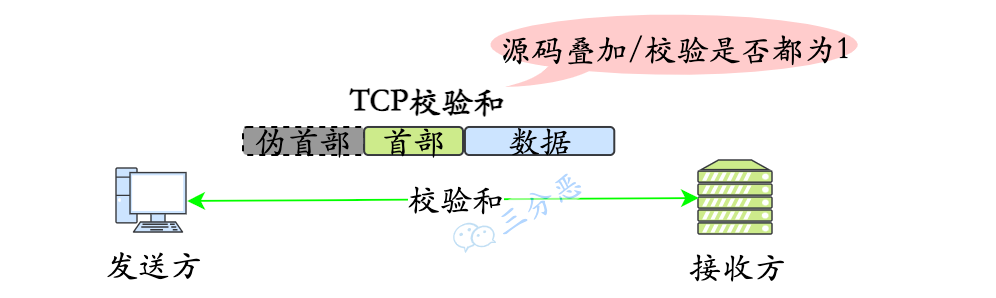
\includegraphics[width=0.9\textwidth]{./Chapter4/q44_2.png}
\caption{TCP 校验和}
\label{fig44_2}
\end{figure}

\newpage
\begin{note} \textbf{序列号/确认应答} \end{note}
TCP 给发送的每一个包进行编号,接收方会对收到的包进行应答,发送方就会知道接收方是否收到对应的包,如果发现没有收到,就会重发,这样就能保证数据的完整性。就像老师上课,会问一句,这一章听懂了吗?没听懂再讲一遍。

\begin{figure}[htbp]
\centering
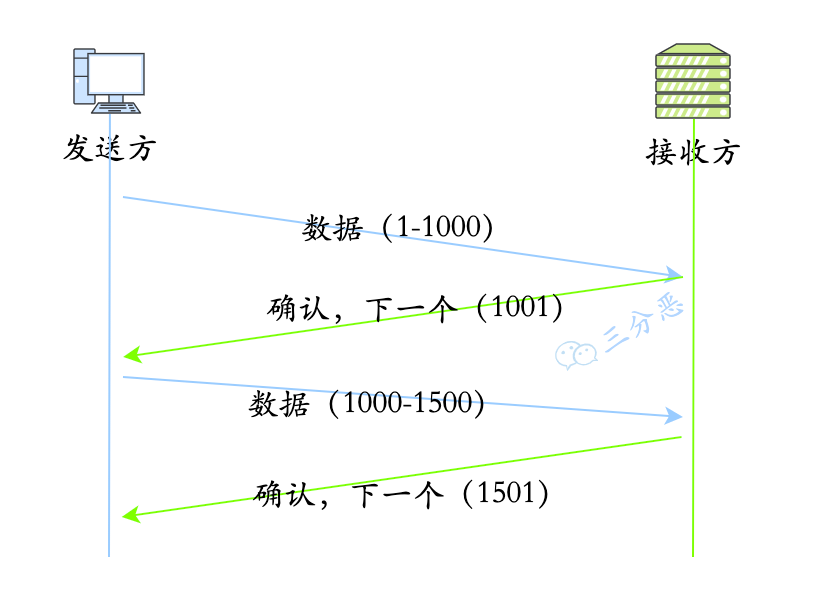
\includegraphics[width=0.7\textwidth]{./Chapter4/q44_3.png}
\caption{序列号/确认应答}
\label{fig44_3}
\end{figure}

\begin{note} \textbf{流量控制} \end{note}
TCP 连接的每一方都有固定大小的缓冲空间,TCP的接收端只允许发送端发送接收端缓冲区能接纳的数据。当接收方来不及处理发送方的数据,能提示发送方降低发送的速率,防止包丢失。TCP 使用的流量控制协议是可变大小的滑动窗口协议。 (TCP 利用滑动窗口实现流量控制)
\begin{figure}[htbp]
\centering
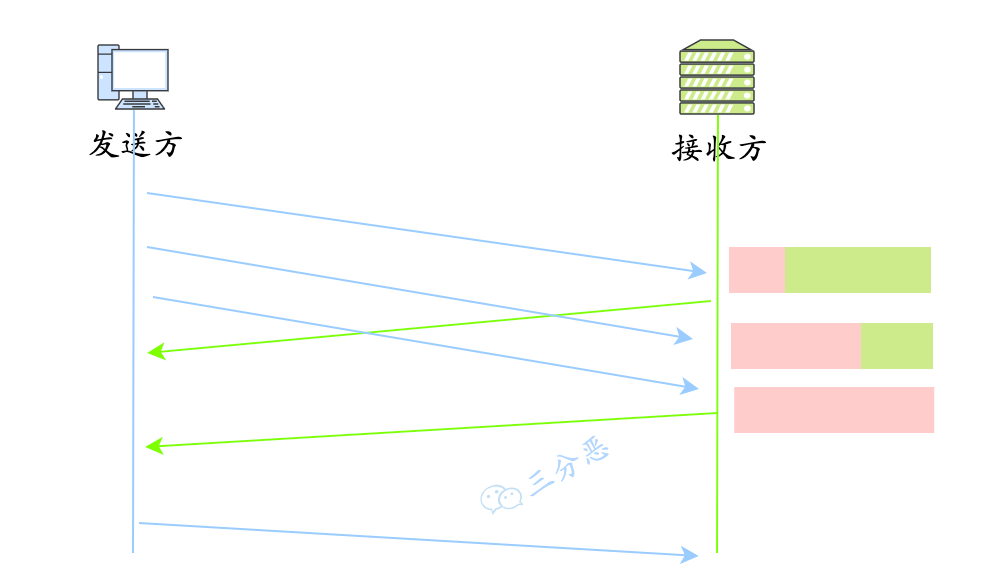
\includegraphics[width=0.9\textwidth]{./Chapter4/q44_4.png}
\caption{滑动窗口简图}
\label{fig44_4}
\end{figure}

\begin{note} \textbf{最大消息长度} \end{note}
在建立 TCP 连接的时候,双方约定一个最大的长度(MSS)作为发送的单位,重传的时候也是以这个单位来进行重传。理想的情况下是该长度的数据刚好不被网络层分块。
\begin{figure}[htbp]
\centering
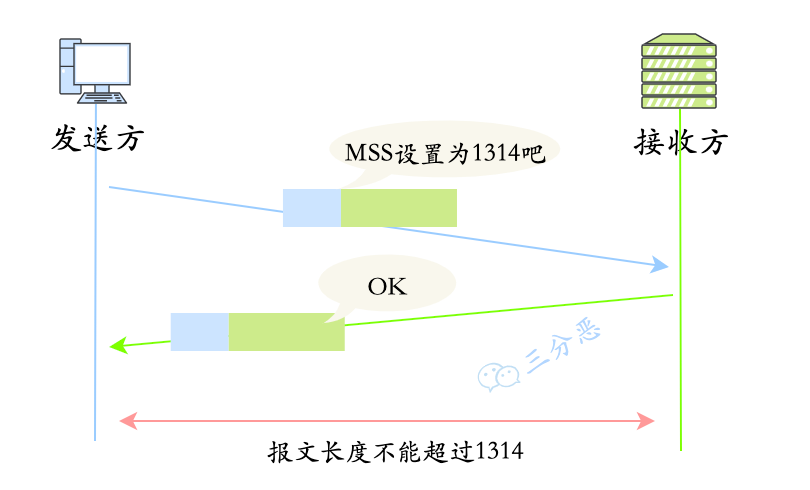
\includegraphics[width=0.7\textwidth]{./Chapter4/q44_5.png}
\caption{最大消息长度}
\label{fig44_5}
\end{figure}

\begin{note} \textbf{超时重传} \end{note}
如果网络非常拥堵,此时再发送数据就会加重网络负担,那么发送的数据段很可能超过了最大生存时间也没有到达接收方,就会产生丢包问题。为此 TCP 引入慢启动机制,先发出少量数据,就像探路一样,先摸清当前的网络拥堵状态后,再决定按照多大的速度传送数据。
\begin{figure}[htbp]
\centering
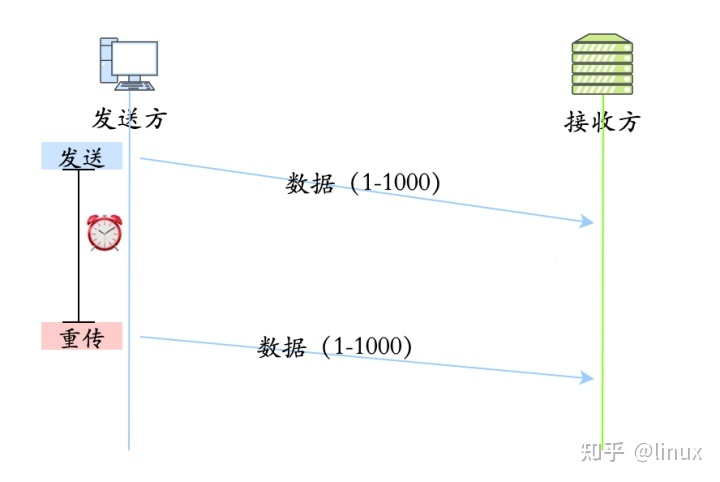
\includegraphics[width=0.7\textwidth]{./Chapter4/q44_6.jpg}
\caption{超时重传}
\label{fig44_6}
\end{figure}

\begin{note} \textbf{拥塞控制} \end{note}
如果网络非常拥堵,此时再发送数据就会加重网络负担,那么发送的数据段很可能超过了最大生存时间也没有到达接收方,就会产生丢包问题。为此 TCP 引入慢启动机制,先发出少量数据,就像探路一样,先摸清当前的网络拥堵状态后,再决定按照多大的速度传送数据。
\begin{figure}[htbp]
\centering
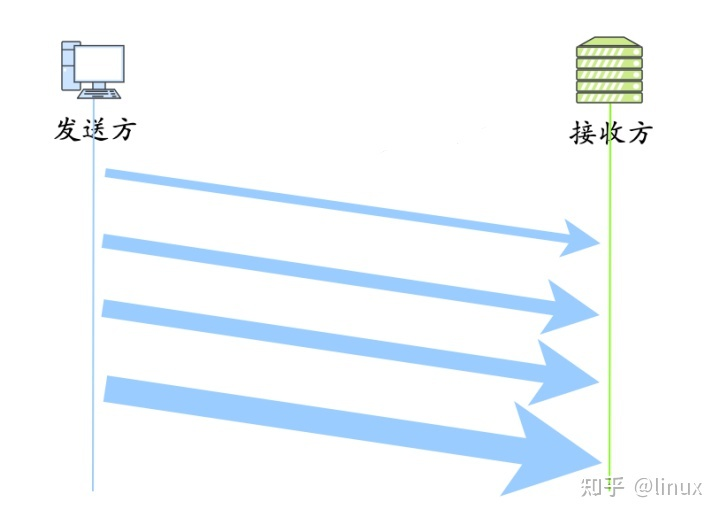
\includegraphics[width=0.6\textwidth]{./Chapter4/q44_7.jpg}
\caption{拥塞控制}
\label{fig44_7}
\end{figure}

\end{solution}

%--------------------------------------------- 问题45 ------------------------------------
\begin{custom}{问题45}
说说 TCP 的流量控制?
\end{custom}
\begin{solution}
TCP 提供了一种机制,可以让发送端根据接收端的实际接收能力控制发送的数据量,这就是流量控制。

TCP 通过滑动窗口来控制流量,我们看下图所示的简要流程:
\begin{figure}[htbp]
\centering
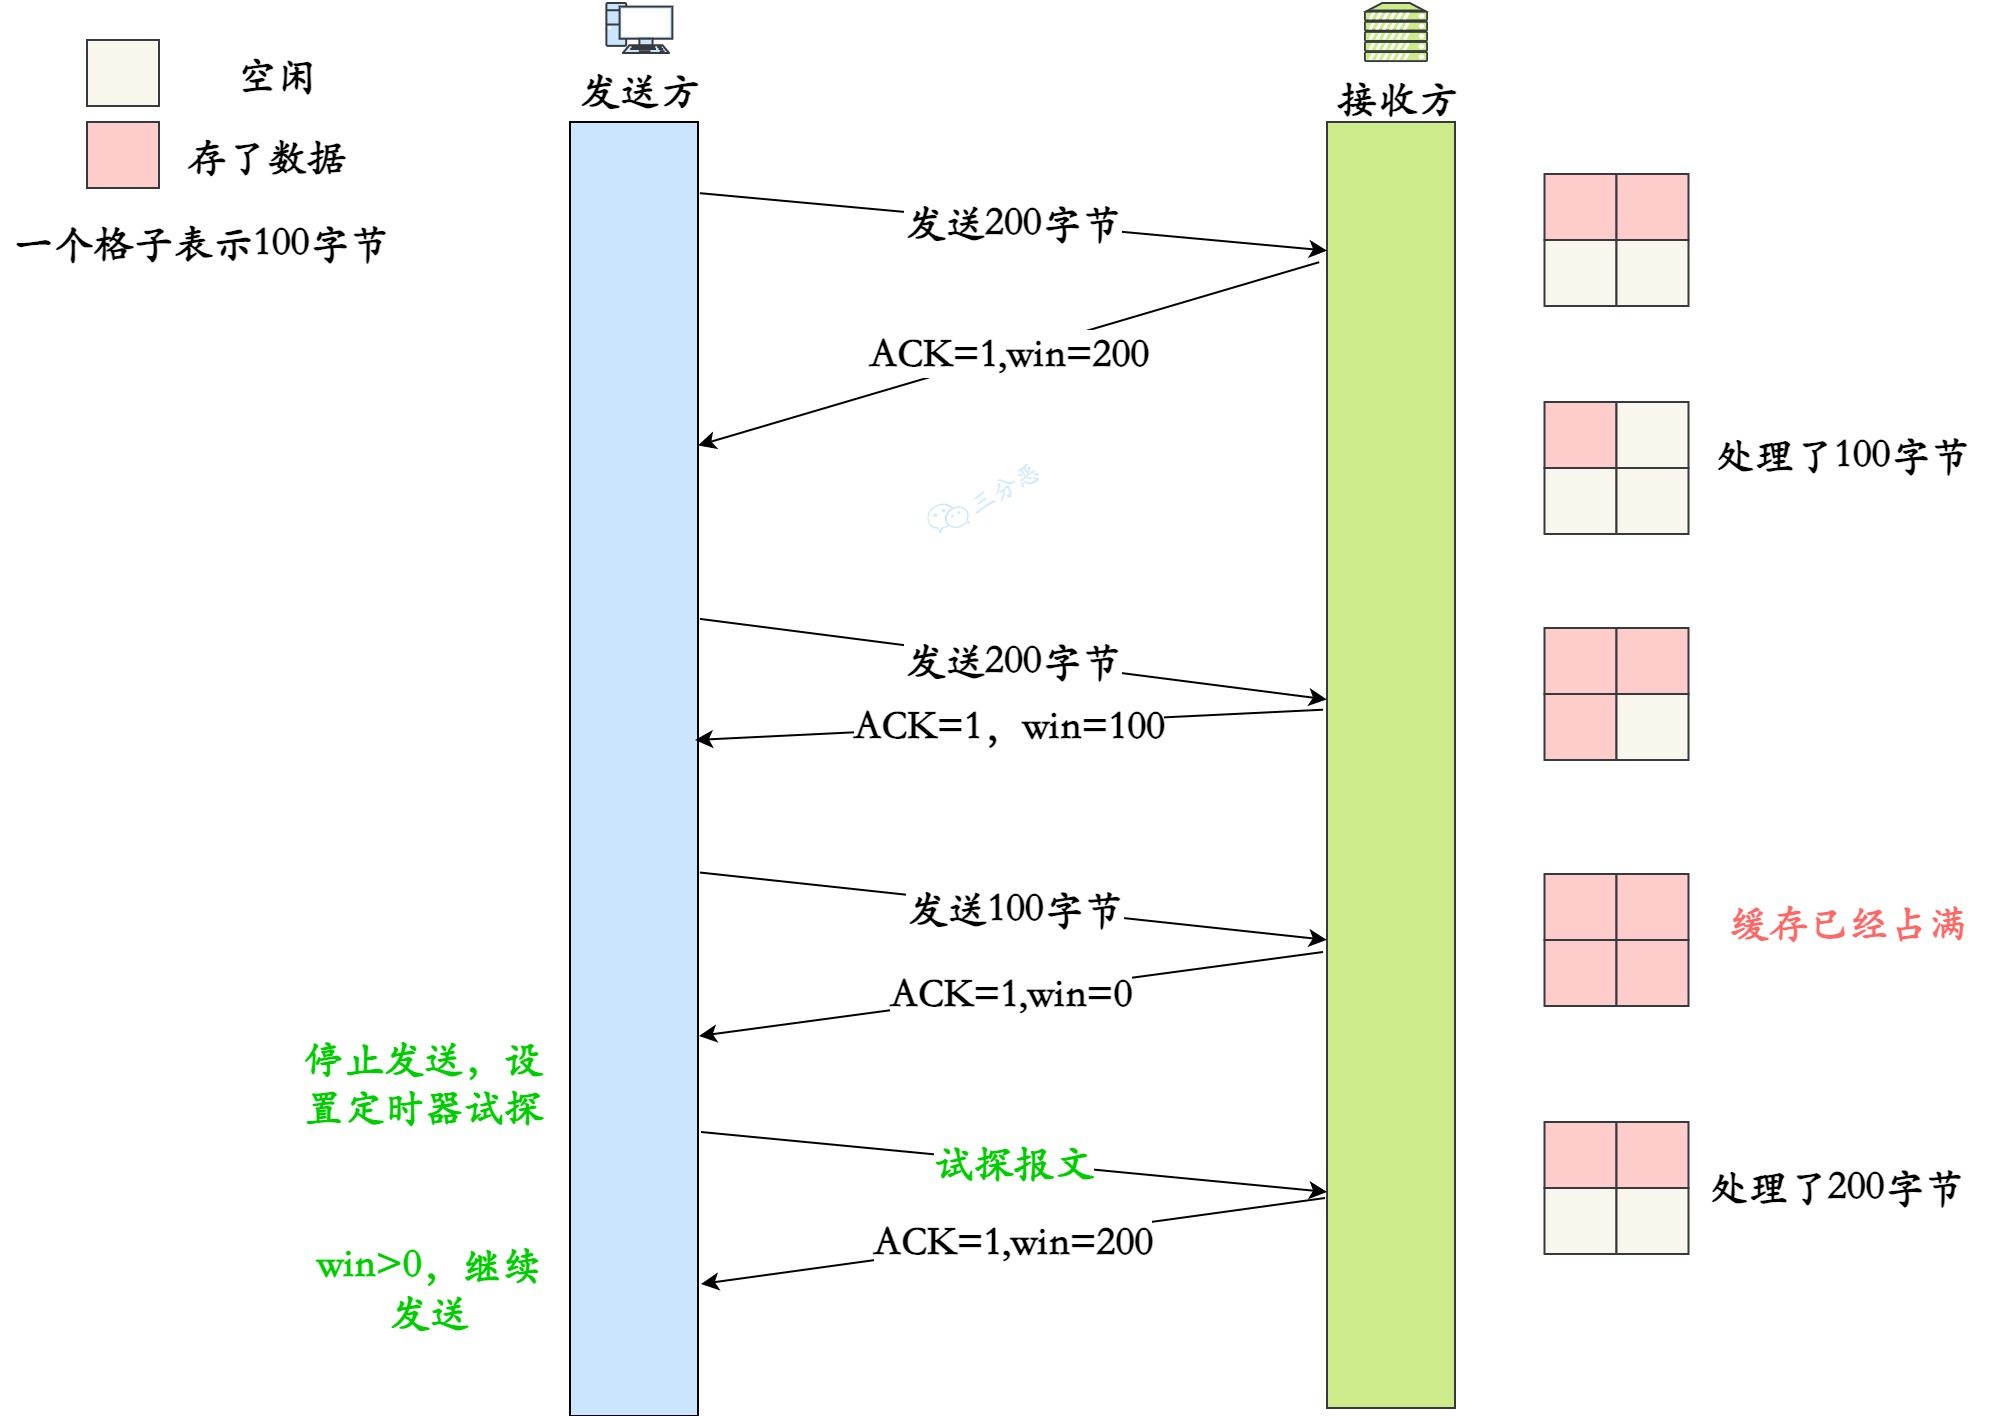
\includegraphics[width=0.95\textwidth]{./Chapter4/q45_1.png}
\caption{TCP 流量控制}
\label{fig45_1}
\end{figure}

\begin{enumerate}
	\item 首先双方三次握手,初始化各自的窗口大小,均为 400 个字节
	\item 假如当前发送方给接收方发送了 200 个字节,那么,发送方的 SND.NXT 会右移 200 个字节,也就是说当前的可用窗口减少了 200 个字节。
	\item 接受方收到后,放到缓冲队列里面,REV.WND =400-200=200 字节,所以 win=200 字节返回给发送方。接收方会在 ACK 的报文首部带上缩小后的滑动窗口 200 字节
	\item 发送方又发送 200 字节过来,200 字节到达,继续放到缓冲队列。不过这时候,由于大量负载的原因,接受方处理不了这么多字节,只能处理 100 字节,剩余的 100 字节继续放到缓冲队列。这时候,REV.WND = 400-200-100=100 字节,即 win=100 返回发送方。
	\item 发送方继续发送 100 字节过来,这时候,接收窗口 win 变为 0。
	\item 发送方停止发送,开启一个定时任务,每隔一段时间,就去询问接受方,直到 win 大于 0,才继续开始发送。
\end{enumerate}
\end{solution}


%--------------------------------------------- 问题46 ------------------------------------
\begin{custom}{问题46}
详细说说 TCP 的滑动窗口?
\end{custom}
\begin{solution}
TCP 发送一个数据,如果需要收到确认应答,才会发送下一个数据。这样的话就会有个缺点:效率会比较低。

“用一个比喻,我们在微信上聊天,你打完一句话,我回复一句之后,你才能打下一句。假如我没有及时回复呢?你是把话憋着不说吗?然后傻傻等到我回复之后再接着发下一句?”

为了解决这个问题,TCP 引入了 窗口,它是操作系统开辟的一个缓存空间。窗口大小值表示无需等待确认应答,而可以继续发送数据的最大值。

TCP 头部有个字段叫 win,也即那个 16 位的窗口大小,它告诉对方本端的 TCP 接收缓冲区还能容纳多少字节的数据,这样对方就可以控制发送数据的速度,从而达到流量控制的目的。

“通俗点讲,就是接受方每次收到数据包,在发送确认报文的时候,同时告诉发送方,自己的缓存区还有多少空余空间,缓冲区的空余空间,我们就称之为接受窗口大小。这就是 win。”

TCP 滑动窗口分为两种: 发送窗口和接收窗口。

\begin{note} \textbf{发送窗口} \end{note}
发送端的滑动窗口包含四大部分,如下:
\begin{itemize}
	\item 已发送且已收到 ACK 确认
	\item 已发送但未收到 ACK 确认
	\item 未发送但可以发送
	\item 未发送也不可以发送
\end{itemize}

发送端滑动窗口如下图\ref{fig46_1} 所示:

\begin{figure}[htbp]
\centering
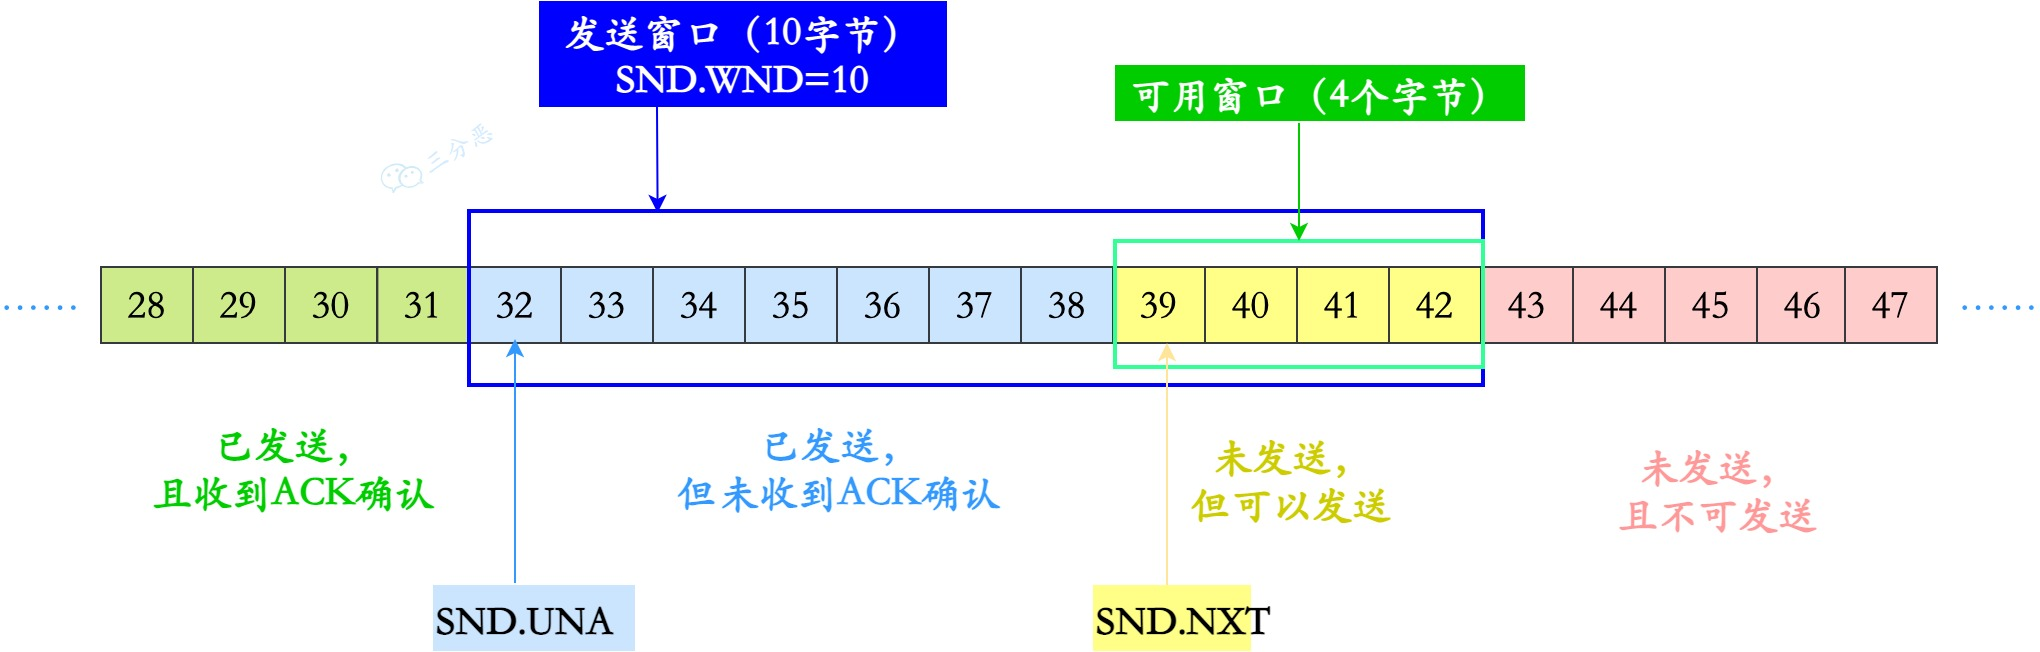
\includegraphics[width=0.85\textwidth]{./Chapter4/q46_1.png}
\caption{发送端口窗口}
\label{fig46_1}
\end{figure}
其中,

\begin{itemize}
	\item 深蓝色框里就是发送窗口。
	\item SND.WND: 表示发送窗口的大小, 上图虚线框的格子数是 10个,即发送窗口大小是 10。
	\item SND.NXT:下一个发送的位置,它指向未发送但可以发送的第一个字节的序列号。
	\item SND.UNA: 一个绝对指针,它指向的是已发送但未确认的第一个字节的序列号。
\end{itemize}

\begin{note} \textbf{接收窗口} \end{note}

接收方的滑动窗口包含三大部分,如下:
\begin{itemize}
	\item 已成功接收并确认
	\item 未收到数据但可以接收
	\item 未收到数据并不可以接收的数据
\end{itemize}

接收窗口如下图\ref{fig46_2} 所示:
\begin{figure}[htbp]
\centering
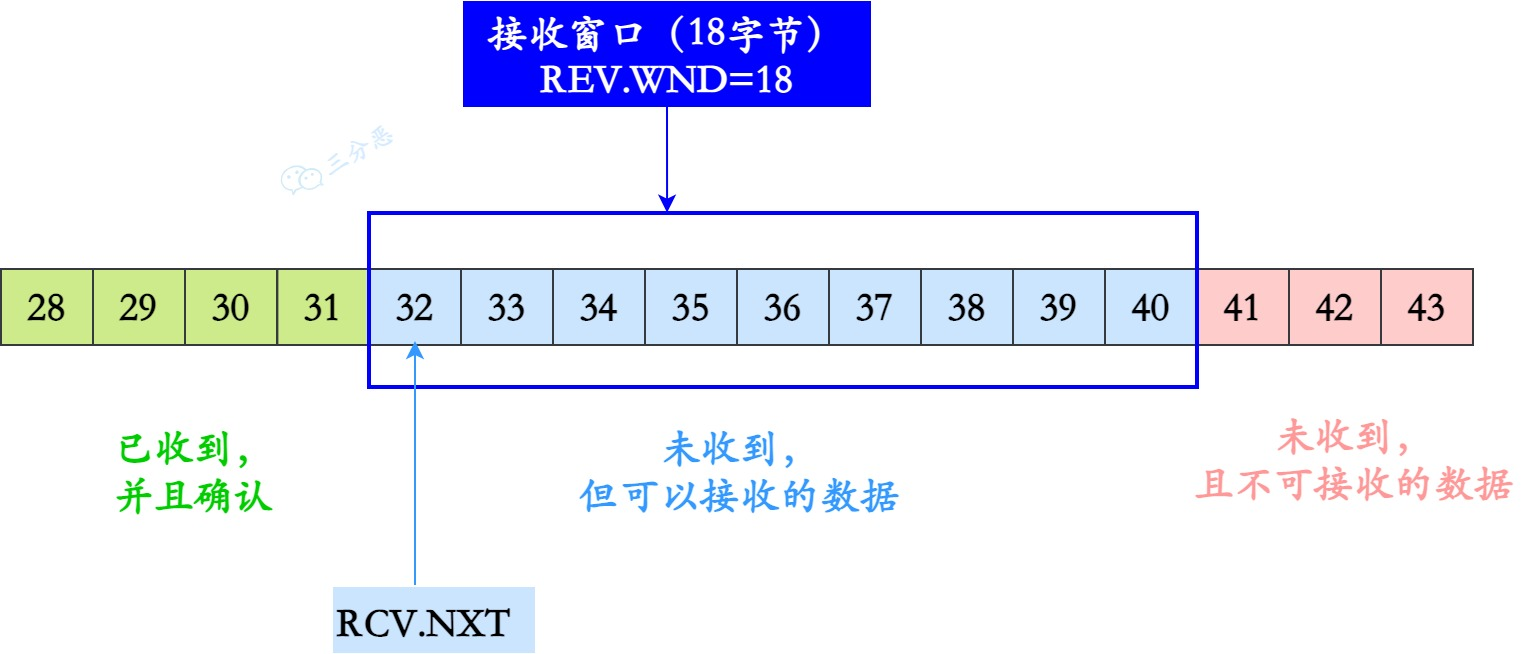
\includegraphics[width=0.8\textwidth]{./Chapter4/q46_2.png}
\caption{接收端口窗口}
\label{fig46_2}
\end{figure}

其中,
\begin{itemize}
	\item 蓝色框内,就是接收窗口。
	\item REV.WND: 表示接收窗口的大小, 上图虚线框的格子就是 9 个。
	\item REV.NXT: 下一个接收的位置,它指向未收到但可以接收的第一个字节的序列号。
\end{itemize}

\end{solution}


%--------------------------------------------- 问题47 ------------------------------------
\begin{custom}{问题47}
了解Nagle 算法和延迟确认吗?
\end{custom}

\begin{solution}
\begin{note} \textbf{Nagle 算法和延迟确认是干什么的?} \end{note}
\begin{figure}[htbp]
\centering
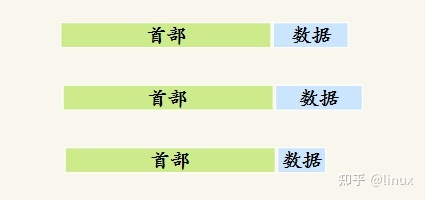
\includegraphics[width=0.5\textwidth]{./Chapter4/q47_1.png}
\caption{报文中有效数据越来越低}
\label{fig47_1}
\end{figure}

当我们 TCP 报文的承载的数据非常下的时候,例如几个字节,那么整个网络的效率是很低的,因为每个 TCP 报文中都会有 20 个字节的 TCP 头部,也会有 20 个字节的 IP 头部,而数据只有几个字节,所以在整个报文中有效数据占有的比例就会非常低,如上图\ref{fig47_1} 所示。

这就好像快递员开着大货车送一个小包裹一样浪费。那么就出现了常见的两种策略,来减少小报文的传输,分别是:
\begin{itemize}
	\item Nagle 算法
	\item 延迟确认
\end{itemize}

\begin{note} \textbf{Nagle 算法} \end{note}
Nagle 算法:任意时刻,最多只能有一个未被确认的小段。所谓 “小段”,指的是小于 MSS 尺寸的数据块,所谓 “未被确认”,是指一个数据块发送出去后,没有收到对方发送的 ACK 确认该数据已收到。

Nagle 算法的策略:
\begin{itemize}
	\item 没有已发送未确认报文时,立刻发送数据。
	\item 存在未确认报文时,直到「没有已发送未确认报文」或「数据长度达到 MSS 大小」时,再发送数据。
\end{itemize}

只要没满足上面条件中的一条,发送方一直在囤积数据,直到满足上面的发送条件。

\begin{note} \textbf{延迟确认} \end{note}
事实上当没有携带数据的 ACK,它的网络效率也是很低的,因为它也有 40 个字节的 IP 头 和 TCP 头,但却没有携带数据报文。为了解决 ACK 传输效率低问题,所以就衍生出了 TCP 延迟确认。

TCP 延迟确认的策略:
\begin{itemize}
	\item 当有响应数据要发送时,ACK 会随着响应数据一起立刻发送给对方;
	\item 当没有响应数据要发送时,ACK 将会延迟一段时间,以等待是否有响应数据可以一起发送;
	\item 如果在延迟等待发送 ACK 期间,对方的第二个数据报文又到达了,这时就会立刻发送 ACK。
\end{itemize}
一般情况下,\textbf{Nagle 算法和延迟确认不能一起使用},Nagle 算法意味着延迟发,延迟确认意味着延迟接收,两个凑在一起就会造成更大的延迟,会产生性能问题。

\end{solution}


%--------------------------------------------- 问题48 ------------------------------------
\begin{custom}{问题48}
说说TCP 的拥塞控制?
\end{custom}
\begin{solution}
\begin{note} \textbf{什么是拥塞控制?不是有了流量控制吗?} \end{note}
前面的流量控制是避免发送方的数据填满接收方的缓存,但是并不知道整个网络之中发生了什么。一般来说,计算机网络都处在一个共享的环境。因此也有可能会因为其他主机之间的通信使得网络拥堵。

在网络出现拥堵时,如果继续发送大量数据包,可能会导致数据包时延、丢失等,这时 TCP 就会重传数据,但是一重传就会导致网络的负担更重,于是会导致更大的延迟以及更多的丢包,这个情况就会进入恶性循环被不断地放大....

所以,TCP 不能忽略整个网络中发生的事,它被设计成一个无私的协议,当网络发生拥塞时,TCP 会自我牺牲,降低发送的数据流。

于是,就有了拥塞控制,控制的目的就是避免发送方的数据填满整个网络。

就像是一个水管,不能让太多的水(数据流)流入水管,如果超过水管的承受能力,水管会被撑爆(丢包),如下图\ref{fig48_1} 所示。
\begin{figure}[htbp]
\centering
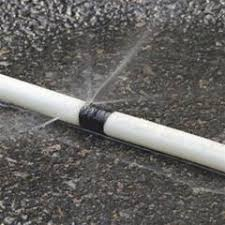
\includegraphics[width=0.4\textwidth]{./Chapter4/q48_1.png}
\caption{破解的水管}
\label{fig48_1}
\end{figure}

发送方维护一个拥塞窗口 cwnd(congestion window)的变量,调节所要发送数据的量。

\begin{note} \textbf{什么是拥塞窗口?和发送窗口有什么关系呢?} \end{note}
拥塞窗口 cwnd 是发送方维护的一个的状态变量,它会根据网络的拥塞程度动态变化的。

发送窗口 swnd 和接收窗口 rwnd 是约等于的关系,那么由于加入了拥塞窗口的概念后,此时发送窗口的值是 swnd = min(cwnd, rwnd),也就是拥塞窗口和接收窗口中的最小值。

拥塞窗口 cwnd 变化的规则:
\begin{itemize}
	\item 只要网络中没有出现拥塞, cwnd 就会增大;
	\item 但网络中出现了拥塞, cwnd 就减少;
\end{itemize}

\begin{note} \textbf{拥塞控制有哪些常用算法?} \end{note}
拥塞控制主要有这几种常用算法:

\begin{itemize}
	\item 慢启动
	\item 拥塞避免
	\item 拥塞发生
	\item 快速恢复
\end{itemize}

\begin{note} \textbf{慢启动算法} \end{note}
慢启动算法,慢慢启动。

它表示 TCP 建立连接完成后,一开始不要发送大量的数据,而是先探测一下网络的拥塞程度。由小到大逐渐增加拥塞窗口的大小,如果没有出现丢包,每收到一个 ACK,就将拥塞窗口 cwnd 大小就加 1(单位是 MSS)。每轮次发送窗口增加一倍,呈指数增长,如果出现丢包,拥塞窗口就减半,进入拥塞避免阶段。

举个例子:
\begin{itemize}
	\item 连接建立完成后,一开始初始化 cwnd = 1 ,表示可以传一个 MSS 大小的数据。
	\item 当收到一个 ACK 确认应答后,cwnd 增加 1,于是一次能够发送 2 个
	\item 当收到 2 个的 ACK 确认应答后, cwnd 增加 2,于是就可以比之前多发2 个,所以这一次能够发送 4 个
	\item 当这 4 个的 ACK 确认到来的时候,每个确认 cwnd 增加 1, 4 个确认 cwnd 增加 4,于是就可以比之前多发4 个,所以这一次能够发送 8 个。
\end{itemize}

就如下图\ref{fig48_3} 所示:
\begin{figure}[htbp]
\centering
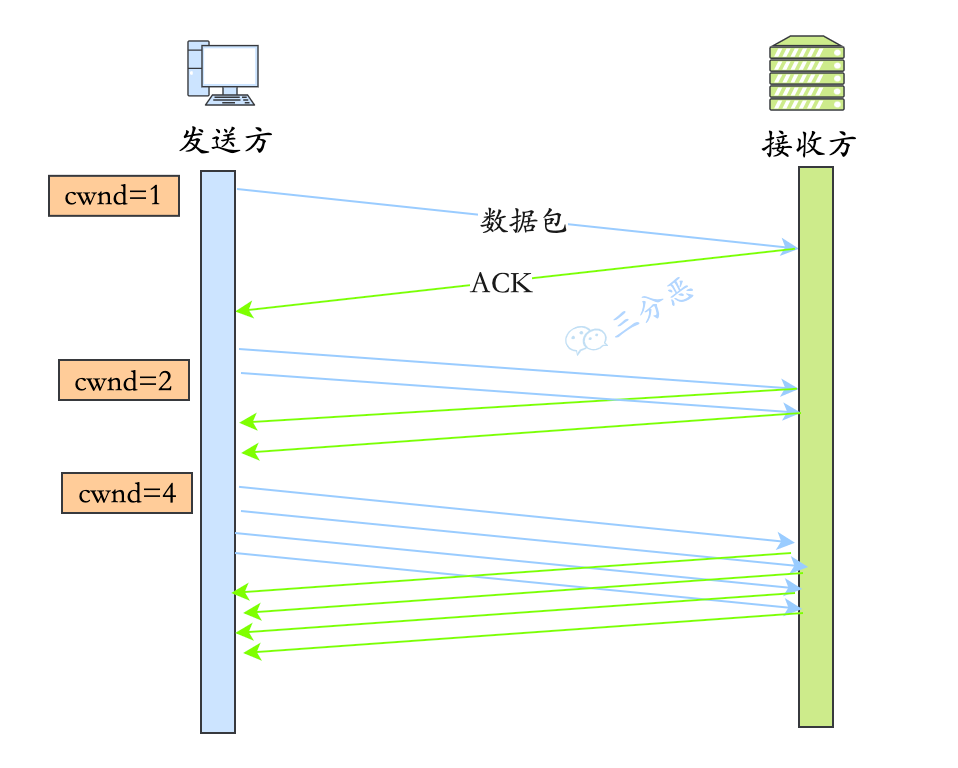
\includegraphics[width=0.65\textwidth]{./Chapter4/q48_3.png}
\caption{慢启动算法}
\label{fig48_3}
\end{figure}

发包的个数是指数性的增长,如下图\ref{fig48_4} 所示。
\begin{figure}[htbp]
\centering
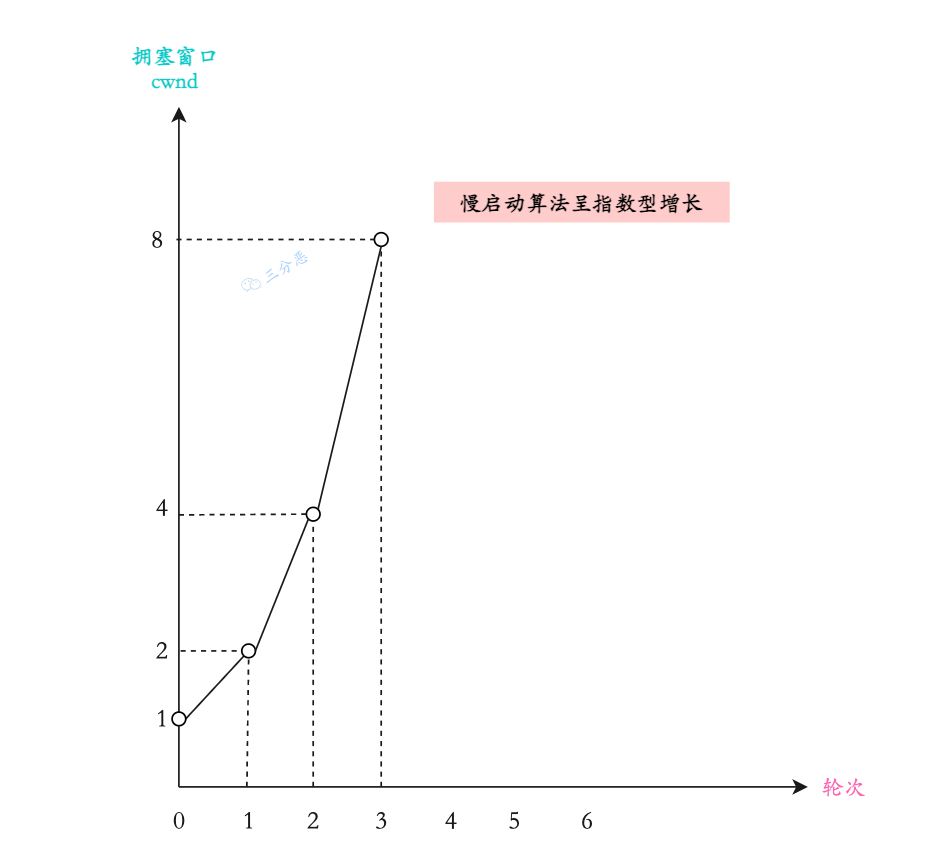
\includegraphics[width=0.75\textwidth]{./Chapter4/q48_4.png}
\caption{慢启动呈指数型增长}
\label{fig48_4}
\end{figure}

为了防止 cwnd 增长过大引起网络拥塞,还需设置一个慢启动阀值 ssthresh(slow start threshold)状态变量。当cwnd到达该阀值后,就好像水管被关小了水龙头一样,减少拥塞状态。即当 cwnd >ssthresh 时,进入了拥塞避免算法。

\begin{note} \textbf{拥塞避免算法} \end{note}
一般来说,慢启动阀值 ssthresh 是 65535 字节,cwnd 到达慢启动阀值后
\begin{itemize}
	\item 每收到一个 ACK 时,cwnd = cwnd + 1/cwnd
	\item 当每过一个 RTT 时,cwnd = cwnd + 1
\end{itemize}

显然这是一个线性上升的算法,避免过快导致网络拥塞问题。

接着上面慢启动的例子,假定 ssthresh 为 8。当 8 个 ACK 应答确认到来时,每个确认增加 1/8,8 个 ACK 确认 cwnd 一共增加 1,于是这一次能够发送 9个 MSS 大小的数据,变成了线性增长,如下图\ref{fig48_5} 所示。

\begin{figure}[htbp]
\centering
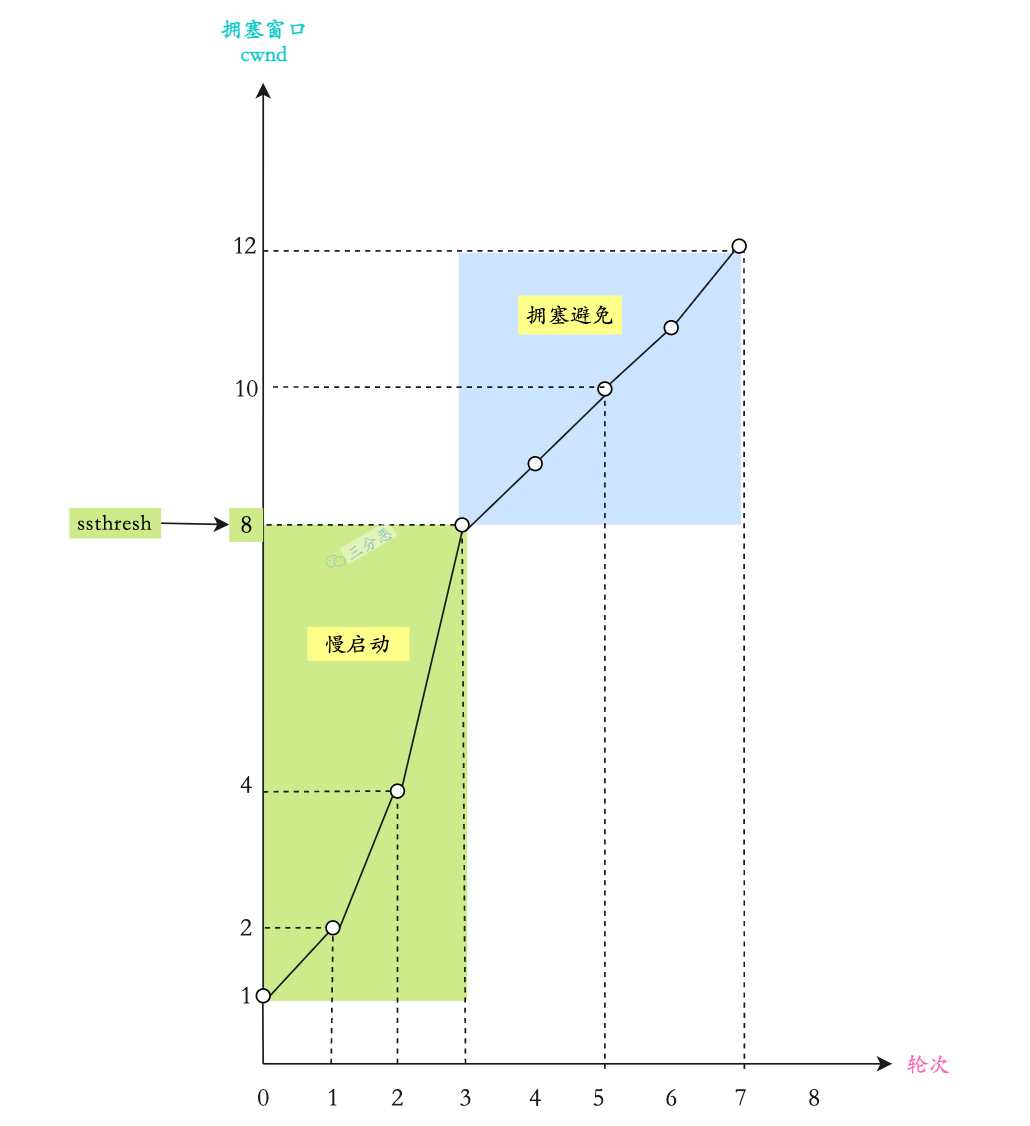
\includegraphics[width=0.75\textwidth]{./Chapter4/q48_5.png}
\caption{拥塞避免算法}
\label{fig48_5}
\end{figure}

\begin{note} \textbf{拥塞发生算法} \end{note}
当网络拥塞发生丢包时,会有两种情况: \textbf{RTO 超时重传}和\textbf{快速重传}。

如果是发生了 RTO 超时重传,就会使用拥塞发生算法,如下图\ref{fig48_6} 所示:
\begin{itemize}
	\item 慢启动阀值 sshthresh = cwnd /2
	\item cwnd 重置为 1
	\item 进入新的慢启动过程
\end{itemize}

\begin{figure}[htbp]
\centering
\includegraphics[width=0.9\textwidth]{./Chapter4/q48_6.png}
\caption{拥塞发生算法}
\label{fig48_6}
\end{figure}

这种方式就像是飙车的时候急刹车,还飞速倒车,这。。。

其实还有更好的处理方式,就是快速重传。发送方收到 3 个连续重复的 ACK 时,就会快速地重传,不必等待 RTO 超时再重传。

发生快速重传的拥塞发生算法:

\begin{itemize}
	\item 拥塞窗口大小 cwnd = cwnd/2
	\item 慢启动阀值 ssthresh = cwnd
	\item 进入快速恢复算法
\end{itemize}

\begin{note} \textbf{快速恢复算法} \end{note}
快速重传和快速恢复算法一般同时使用。快速恢复算法认为,还有 3 个重复 ACK 收到,说明网络也没那么糟糕,所以没有必要像 RTO 超时那么强烈。

正如前面所说,进入快速恢复之前,cwnd 和 sshthresh 已被更新:
\begin{itemize}
	\item cwnd = cwnd/2
	\item sshthresh = cwnd
\end{itemize}

然后,进入快速恢复算法如下图\ref{fig48_7} 所示:
\begin{itemize}
	\item cwnd = sshthresh + 3
	\item 重传重复的那几个 ACK(即丢失的那几个数据包)
	\item 如果再收到重复的 ACK,那么 cwnd = cwnd +1
	\item 如果收到新数据的 ACK 后, cwnd = sshthresh。因为收到新数据的 ACK,表明恢复过程已经结束,可以再次进入了拥塞避免的算法了。
\end{itemize}

\begin{figure}[htbp]
\centering
\includegraphics[width=0.95\textwidth]{./Chapter4/q48_7.png}
\caption{拥塞发生算法}
\label{fig48_7}
\end{figure}

\end{solution}

%--------------------------------------------- 问题49 ------------------------------------
\begin{custom}{问题49}
说一说 TCP 重传机制?
\end{custom}
\begin{solution}
重传包括超时重传、快速重传、带选择确认的重传(SACK)、重复 SACK 四种。
\begin{figure}[!h]
\centering
\includegraphics[width=0.35\textwidth]{./Chapter4/q49_1.png}
\caption{TCP 重传分类}
\label{fig49_1}
\end{figure}

\newpage
\begin{note} \textbf{超时重传} \end{note}

超时重传,是 TCP 协议保证数据可靠性的另一个重要机制,其原理是在发送某一个数据以后就开启一个计时器,在一定时间内如果没有得到发送的数据报的 ACK 报文,那么就重新发送数据,直到发送成功为止。

那么\mybox[blue]{超时时间应该设置为多少呢?}先来看下什么叫 RTT(Round-Trip Time,往返时间),如下图\ref{fig49_2} 所示。

\begin{figure}[!h]
\centering
\includegraphics[width=0.7\textwidth]{./Chapter4/q49_2.png}
\caption{RTT 往返时间}
\label{fig49_2}
\end{figure}

\textbf{RTT} 就是数据完全发送完,到收到确认信号的时间,即数据包的一次往返时间。\text{超时重传时间,就是 RTO(Retransmission Timeout)}。那么,RTO 到底设置多大呢?

\textbf{如果 RTO 设置很大},等了很久都没重发,这样肯定就不行。\textbf{如果 RTO 设置很小},那很可能数据都没有丢失,就开始重发了,这会导致网络阻塞,从而恶性循环,导致更多的超时出现。一般来说,RTO 略微大于 RTT,效果是最佳的。

其实,RTO 有个标准方法的计算公式,也叫 Jacobson / Karels 算法,如下面所示 。

\begin{myDefinition}{Jacobson / Karels 算法}{JK}
(1) 首先计算 SRTT(即计算平滑的 RTT)
\begin{equation}
   \label{eq:1}
   \text{SRTT = (1 - α) * SRTT + α * RTT  //求 SRTT 的加权平均}
\end{equation}

(2) 其次,计算 RTTVAR (round-trip time variation)
\begin{equation}
   \label{eq:2}
   \text{RTTVAR = (1 - β) * RTTVAR + β * (|RTT - SRTT|) //计算 SRTT 与真实值的差距}
\end{equation}

(3) 最后,得出最终的 RTO
\begin{equation}
   \label{eq:2}
   \text{RTO = µ * SRTT } + \sigma \text{* RTTVAR  =  SRTT + 4·RTTVAR  }
\end{equation}

在 Linux 下,α = 0.125,β = 0.25, μ = 1,$\sigma = 4$。别问这些参数是怎么来的,它们是大量实践,调出的最优参数。
\end{myDefinition}
超时重传不是十分完美的重传方案,它有这些缺点:

\begin{itemize}
	\item 当一个报文丢失时,会等待一定的超时周期,才重传分组,增加了端到端的时延。
	\item 当一个报文丢失时,在其等待超时的过程中,可能会出现这种情况:其后的报文段已经被接收端接收但却迟迟得不到确认,发送端会认为也丢失了,从而引起不必要的重传,既浪费资源也浪费时间。
\end{itemize}

并且,对于 TCP,如果发生一次超时重传,时间间隔下次就会加倍。

\end{solution}

\begin{note} \textbf{快速重传} \end{note}
TCP 还有另外一种快速重传(Fast Retransmit)机制,它不以时间为驱动,而是以数据驱动重传。它不以时间驱动,而是以数据驱动。它是基于接收端的反馈信息来引发重传的。可以用它来解决超时重发的时间等待问题,快速重传流程如下图所示:

\begin{figure}[!h]
\centering
\includegraphics[width=0.7\textwidth]{./Chapter4/q49_3.png}
\caption{快速重传流程}
\label{fig49_3}
\end{figure}

在上图,发送方发出了 1,2,3,4,5 份数据:

\begin{itemize}
	\item 第一份 Seq1 先送到了,于是就 Ack 回 2;
	\item 结果 Seq2 因为某些原因没收到,Seq3 到达了,于是还是 Ack 回 2;
	\item 后面的 Seq4 和 Seq5 都到了,但还是 Ack 回 2,因为 Seq2 还是没有收到;
	\item 发送端收到了三个 Ack = 2 的确认,知道了 Seq2 还没有收到,就会在定时器过期之前,重传丢失的 Seq2。
	\item 最后,收到了 Seq2,此时因为 Seq3,Seq4,Seq5 都收到了,于是 Ack 回 6 。
\end{itemize}

快速重传机制只解决了一个问题,就是超时时间的问题,但是它依然面临着另外⼀个问题。就是重传的时候,是重传之前的一个,还是重传所有的问题。

比如对于上面的例子,是重传 Seq2 呢?还是重传 Seq2、Seq3、Seq4、Seq5 呢?因为发送端并不清楚这连续的三个 Ack 2 是谁传回来的。根据 TCP 不同的实现,以上两种情况都是有可能的。可见,这时一把双刃剑。为了解决不知道该重传哪些 TCP 报文,于是就有 SACK 方法。

\begin{note} \textbf{带选择确认的重传(SACK)} \end{note}

为了解决应该重传多少个包的问题? TCP 提供了带选择确认的重传(即 SACK,Selective Acknowledgment)。

SACK 机制就是,在快速重传的基础上,接收方返回最近收到报文段的序列号范围,这样发送方就知道接收方哪些数据包是没收到的。这样就很清楚应该重传哪些数据包。
\begin{figure}[!h]
\centering
\includegraphics[width=0.9\textwidth]{./Chapter4/q49_4.png}
\caption{SACK 机制}
\label{fig49_4}
\end{figure}

如上图中,发送方收到了三次同样的 ACK 确认报文,于是就会触发快速重发机制,通过 SACK 信息发现只有 200— 299 这段数据丢失,则重发时就只选择了这个 TCP 段进行重发。

\begin{note} \textbf{重复 SACK(D-SACK)} \end{note}
D-SACK,英文是 Duplicate SACK,是在 SACK 的基础上做了一些扩展,主要用来告诉发送方,有哪些数据包,自己重复接受了。

DSACK 的目的是帮助发送方判断,是否发生了包失序、ACK 丢失、包重复或伪重传。让 TCP 可以更好的做网络流控。

例如 ACK 丢包导致的数据包重复:
\begin{figure}[!h]
\centering
\includegraphics[width=0.7\textwidth]{./Chapter4/q49_5.jpg}
\caption{ACK 丢包}
\label{fig49_5}
\end{figure}

接收方发给发送方的两个 ACK 确认应答都丢失了,所以发送方超时后,重传第一个数据包(3000 —
3499)

于是接收方发现数据是重复收到的,于是回了一个 SACK = 3000 — 3500,告诉发送方 3000 — 3500 的数据早已被接收了,因为 ACK 都到了 4000 了,已经意味着 4000 之前的所有数据都已收到,所以这个SACK 就代表着 D-SACK 。这样发送方就知道了,数据没有丢,是接收方的 ACK 确认报文丢了。

%--------------------------------------------- 问题50 ------------------------------------
\begin{custom}{问题50}
说说TCP 的粘包和拆包?
\end{custom}
\begin{solution}
TCP 的粘包和拆包更多的是业务上的概念!

\begin{note} \textbf{什么是TCP粘包和拆包?} \end{note}
TCP 是面向流,没有界限的一串数据。TCP 底层并不了解上层业务数据的具体含义,它会根据 TCP 缓冲区的实际情况进行包的划分,所以在业务上认为,一个完整的包可能会被 TCP 拆分成多个包进行发送,也有可能把多个小的包封装成一个大的数据包发送,这就是所谓的 TCP 粘包和拆包问题。

\begin{figure}[!h]
\centering
\includegraphics[width=0.7\textwidth]{./Chapter4/q50_1.png}
\caption{TCP 的粘包和拆包}
\label{fig50_1}
\end{figure}

\begin{note} \textbf{为什么会产生粘包和拆包呢?} \end{note}
\begin{itemize}
	\item 要发送的数据小于 TCP 发送缓冲区的大小,TCP 将多次写入缓冲区的数据一次发送出去,将会发生粘包;
	\item 接收数据端的应用层没有及时读取接收缓冲区中的数据,将发生粘包;
	\item 要发送的数据大于 TCP 发送缓冲区剩余空间大小,将会发生拆包;
	\item 待发送数据大于 MSS(最大报文长度),TCP 在传输前将进行拆包。即 TCP 报文长度 - TCP 头部长度 > MSS。
\end{itemize}

\begin{note} \textbf{那怎么解决呢?} \end{note}
\begin{itemize}
	\item 发送端将每个数据包封装为固定长度;;
	\item 在数据尾部增加特殊字符进行分割;
	\item 将数据分为两部分,一部分是头部,一部分是内容体;其中头部结构大小固定,且有一个字段声明内容体的大小。
\end{itemize}
\end{solution}

\section{UDP 传输协议}
UDP问的不多,基本上是被拿来和TCP比较。

%--------------------------------------------- 问题51 ------------------------------------
\begin{custom}{问题51}
说说 TCP 和 UDP 的区别?
\end{custom}

\begin{solution}
最根本区别:TCP 是面向连接,而 UDP 是无连接。

\begin{figure}[!h]
\centering
\includegraphics[width=0.7\textwidth]{./Chapter4/q51_1.png}
\caption{TCP 和 UDP 区别}
\label{fig51_1}
\end{figure}

可以这么形容:TCP 是打电话,UDP 是大喇叭。
\begin{figure}[!h]
\centering
\includegraphics[width=0.7\textwidth]{./Chapter4/q51_2.png}
\caption{TCP 和 UDP 区别}
\label{fig51_2}
\end{figure}

\begin{note} \textbf{说说TCP和UDP的应用场景?} \end{note}
\textbf{TCP应用场景:} 效率要求相对低,但对准确性要求相对高的场景。因为传输中需要对数据确认、重发、排序等操作,相比之下效率没有UDP高。例如:文件传输(准确高要求高、但是速度可以相对慢)、收发邮件、远程登录。

\textbf{UDP应用场景:} 效率要求相对高,对准确性要求相对低的场景。例如:QQ聊天、在线视频、网络语音电话(即时通讯,速度要求高,但是出现偶尔断续不是太大问题,并且此处完全不可以使用重发机制)、广播通信(广播、多播)。
\end{solution}


%--------------------------------------------- 问题52 ------------------------------------
\begin{custom}{问题52}
为什么QQ采用UDP协议?
\end{custom}

\begin{solution}
PS:这是多年前的老题了,拉出来怀怀旧,关于 QQ 使用的 UDP 协议原因大致如下图\ref{fig52_1} 所示。
\begin{figure}[!h]
\centering
\includegraphics[width=0.7\textwidth]{./Chapter4/q52_1.jpg}
\caption{QQ 使用 UDP}
\label{fig52_1}
\end{figure}

详细地展开来说,使用 UDP 的好处如下:
\begin{itemize}
	\item 首先,QQ 并不是完全基于 UDP 实现。比如在使用 QQ 进行文件传输等活动的时候,就会使用 TCP 作为可靠传输的保证。

	\item 使用 UDP 进行交互通信的好处在于,延迟较短,对数据丢失的处理比较简单。同时,TCP 是一个全双工协议,需要建立连接,所以网络开销也会相对大。

	\item 如果使用 QQ 语音和 QQ 视频的话,UDP的优势就更为突出了,首先延迟较小。最重要的一点是不可靠传输,这意味着如果数据丢失的话,不会有重传。因为用户一般来说可以接受图像稍微模糊一点,声音稍微不清晰一点,但是如果在几秒钟以后再出现之前丢失的画面和声音,这恐怕是很难接受的。

	\item 由于 QQ 的服务器设计容量是海量级的应用,一台服务器要同时容纳十几万的并发连接,因此服务器端只有采用 UDP 协议与客户端进行通讯才能保证这种超大规模的服务
\end{itemize}

简单总结一下:UDP 协议是无连接方式的协议,它的效率高,速度快,占资源少,对服务器的压力比较小。但是其传输机制为不可靠传送,必须依靠辅助的算法来完成传输控制。QQ 采用的通信协议以UDP为主,辅以 TCP 协议。

\end{solution}

%--------------------------------------------- 问题53 ------------------------------------
\begin{custom}{问题53}
UDP 协议为什么不可靠?
\end{custom}

\begin{solution}
UDP 在传输数据之前不需要先建立连接,远地主机的运输层在接收到UDP报文后,不需要确认,提供不可靠交付。总结就以下四点:
\begin{itemize}
	\item 不保证消息交付:不确认,不重传,无超时;
	\item 不保证交付顺序:不设置包序号,不重排,不会发生队首阻塞;
	\item 不跟踪连接状态:不必建立连接或重启状态机;
	\item 不进行拥塞控制:不内置客户端或网络反馈机制。
\end{itemize}
\end{solution}

%--------------------------------------------- 问题54 ------------------------------------
\begin{custom}{问题54}
DNS 为什么要用 UDP?
\end{custom}

\begin{solution}
\textbf{更准确地说,DNS 既使用 TCP 又使用 UDP。}

当进行区域传送(主域名服务器向辅助域名服务器传送变化的那部分数据)时会使用 TCP,因为数据同步传送的数据量比一个请求和应答的数据量要多,而TCP允许的报文长度更长,因此为了保证数据的正确性,会使用基于可靠连接的TCP。

当客户端想 DNS 服务器查询域名(域名解析)的时候,一般返回的内容不会超过UDP报文的最大长度,即 512 字节,用 UDP 传输时,不需要创建连接,从而大大提高了响应速度,但这要求域名解析服务器和域名服务器都必须自己处理超时和重传从而保证可靠性。
\end{solution}

\chapter{网络层对应问题}

%--------------------------------------------- 问题55 ------------------------------------
\begin{custom}{问题55}
IP 协议的定义和作用?
\end{custom}

\begin{solution}

\begin{note} \textbf{IP协议是什么?} \end{note}
IP 协议(Internet Protocol)又被称为互联网协议,是支持网间互联的数据包协议,工作在网际层,主要目的就是为了提高网络的可扩展性。

通过网际协议 IP,可以把参与互联的,性能各异的网络看作一个统一的网络。
\begin{figure}[!h]
\centering
\includegraphics[width=0.7\textwidth]{./Chapter5/q55_1.png}
\caption{虚拟 IP 网}
\label{fig55_1}
\end{figure}

和传输层 TCP 相比,IP 协议是一种无连接/不可靠、尽力而为的数据包传输服务,和 TCP 协议一起构成了 TCP/IP 协议的核心。

\begin{note} \textbf{IP协议有哪些作用?} \end{note}

IP 协议主要有以下几个作用:
\begin{itemize}
	\item \textbf{寻址和路由}:在 IP 数据报中携带源 IP 地址和目的 IP 地址来表示该数据包的源主机和目标主机。IP 数据报在传输过程中,每个中间节点(IP 网关、路由器)只根据网络地址来进行转发,如果中间节点是路由器,则路由器会根据路由表选择合适的路径。IP 协议根据路由选择协议提供的路由信息对 IP 数据报进行转发,直至目标主机。
	\item \textbf{分段和重组}:IP 数据报在传输过程中可能会经过不同的网络,在不同的网络中数据报的最大长度限制是不同的,IP 协议通过给每个 IP 数据报分配一个标识符以及分段与组装的相关信息,使得数据报在不同的网络中能够被传输,被分段后的 IP 数据报可以独立地在网络中进行转发,在达到目标主机后由目标主机完成重组工作,恢复出原来的 IP 数据报。
\end{itemize}

\begin{note} \textbf{传输层协议和网络层协议有什么区别?} \end{note}

网络层协议负责提供主机间的逻辑通信;传输层协议负责提供进程间的逻辑通信。
\end{solution}


%--------------------------------------------- 问题56 ------------------------------------
\begin{custom}{问题56}
IP 地址有哪些分类?
\end{custom}
\begin{solution}
一个IP地址在这鞥个互联网范围内是惟一的,\mybox[gray]{IP 地址 = \{<网络号>,<主机号>\}}。
\begin{itemize}
	\item 网络号:它标志主机所连接的网络地址表示属于互联网的哪一个网络。
	\item 主机号:它标志主机地址表示其属于该网络中的哪一台主机。
\end{itemize}
IP 地址分为 A,B,C,D,E 五大类,如下图 所示:
\begin{itemize}
	\item A 类地址 (1~126):以 0 开头,网络号占前 8 位,主机号占后面 24 位。
	\item B 类地址 (128~191):以 10 开头,网络号占前 16 位,主机号占后面 16 位。
	\item C 类地址 (192~223):以 110 开头,网络号占前 24 位,主机号占后面 8 位。
	\item D 类地址 (224~239):以 1110 开头,保留为多播地址。
	\item E 类地址 (240~255):以 1111开头,保留位为将来使用
\end{itemize}

\begin{figure}[!h]
\centering
\includegraphics[width=1.0\textwidth]{./Chapter5/q56_1.png}
\caption{IP 地址分类}
\label{fig56_1}
\end{figure}
\end{solution}

%--------------------------------------------- 问题57 ------------------------------------
\begin{custom}{问题57}
域名和 IP 的关系?一个 IP 可以对应多个域名吗?
\end{custom}

\begin{solution}
\begin{itemize}
	\item IP 地址在同一个网络中是惟一的,用来标识每一个网络上的设备,其相当于一个人的身份证号;
	\item 域名在同一个网络中也是惟一的,就像是一个人的名字、绰号。
\end{itemize}
假如你有多个不用的绰号,你的朋友可以用其中任何一个绰号叫你,但你的身份证号码却是惟一的。但同时你的绰号也可能和别人重复,假如你不在,有人叫你的绰号,其它人可能就答应了。

\textbf{一个域名可以对应多个 IP,但这种情况 DNS 做负载均衡的,在用户访问过程中,一个域名只能对应一个 IP。而一个 IP 却可以对应多个域名,是一对多的关系。}
\end{solution}

%--------------------------------------------- 问题58 ------------------------------------
\begin{custom}{问题58}
IPV4 地址不够如何解决?
\end{custom}
\begin{solution}
我们知道,IP 地址有 32 位,可以标记 2 的 32 次方个地址,听起来很多,但是全球的网络设备数量已经远远超过这个数字,所以 IPV4 地址已经不够用了,那怎么解决呢?

常用的 4 种办法如下图\ref{fig58_1} 所示:
\begin{figure}[!h]
\centering
\includegraphics[width=0.75\textwidth]{./Chapter5/q58_1.png}
\caption{IPv4 不够解决办法}
\label{fig58_1}
\end{figure}

展开讲上述 4 种办法:
\begin{itemize}
	\item DHCP:动态主机配置协议,动态分配 IP 地址,只给接入网络的设备分配 IP 地址,因此同一个 MAC 地址的设备,每次接入互联网时,得到的 IP 地址不一定是相同的,该协议使得空闲的 IP 地址可以得到充分利用。
	\item CIDR:无类别域间路由。CIDR 消除了传统的 A 类、B 类、C 类地址以及划分子网的概念,因而更加有效地分配 IPv4 的地址空间,但无法从根本上解决地址耗尽的问题。
	\item NAT:网络地址转换协议,我们知道属于不同局域网的主机可以使用相同的 IP 地址,从而一定程度上缓解了 IP 资源枯竭的问题,然而主机在局域网中使用的 IP 地址是不能在公网中使用的,当局域网主机想要与公网主机进行通信时,NAT 方法可以将该主机 IP 地址转换为全球 IP 地址。该协议能够有效解决 IP 地址不足的问题。
	\item IPv6:作为接替IPv4的下一代互联网协议,其可以实现2的128次方个地址,而这个数量级,即使给地球上每一粒沙子都分配一个IP地址也够用,该协议能够从根本上解决IPv4地址不够用的问题。
\end{itemize}

\end{solution}

%--------------------------------------------- 问题59 ------------------------------------
\begin{custom}{问题59}
说下 ARP 协议的工作过程?
\end{custom}
\begin{solution}
ARP 协议,Address Resolution Protocol,地址解析协议,它是用于实现 IP 地址到 MAC 地址的映射,如图\ref{fig59_1} 所示。
\begin{figure}[!h]
\centering
\includegraphics[width=0.75\textwidth]{./Chapter5/q59_1.png}
\caption{ARP 协议作用}
\label{fig59_1}
\end{figure}

IP 地址映射为 MAC 地址的步骤如下:
\begin{enumerate}
	\item 首先,每台主机都会在自己的 ARP 缓冲区中建立一个 ARP 列表,以表示 IP 地址和 MAC 地址的对应关系。
	\item 当源主机需要将一个数据包要发送到目的主机时,会首先检查自己的 ARP 列表,是否存在该 IP 地址对应的 MAC 地址;如果有﹐就直接将数据包发送到这个 MAC 地址;如果没有,就向本地网段发起一个 ARP 请求的广播包,查询此目的主机对应的 MAC 地址。此 ARP 请求的数据包里,包括源主机的 IP 地址、硬件地址、以及目的主机的 IP 地址。
	\item 网络中所有的主机收到这个 ARP 请求后,会检查数据包中的目的 IP 是否和自己的 IP 地址一致。如果不相同,就会忽略此数据包;如果相同,该主机首先将发送端的 MAC 地址和 IP 地址添加到自己的 ARP 列表中,如果 ARP 表中已经存在该 IP 的信息,则将其覆盖,然后给源主机发送一个 ARP 响应数据包,告诉对方自己是它需要查找的 MAC 地址。
	\item 
源主机收到这个 ARP 响应数据包后,将得到的目的主机的 IP 地址和 MAC 地址添加到自己的 ARP 列表中,并利用此信息开始数据的传输。如果源主机一直没有收到 ARP 响应数据包,表示 ARP 查询失败。
\end{enumerate}
\end{solution}
	

%--------------------------------------------- 问题60 ------------------------------------
\begin{custom}{问题60}
为什么既有 IP 地址,又有 MAC 地址?
\end{custom}
\begin{solution}

\begin{figure}[!h]
\centering
\includegraphics[width=0.9\textwidth]{./Chapter5/q60_1.png}
\caption{IP 地址和 MAC 地址}
\label{fig60_1}
\end{figure}

\begin{note} \textbf{MAC 地址和 IP 地址都有什么作用?} \end{note}
\textbf{MAC 地址}是数据链路层和物理层使用的地址,是写在网卡上的物理地址,用来定义网络设备的位置,不可变更。

\textbf{IP 地址}是网络层和以上各层使用的地址,是一种逻辑地址。IP 地址用来区别网络上的计算机。

\begin{note} \textbf{为什么有了 MAC 地址还需要 IP 地址?} \end{note}
如果我们只使用 MAC 地址进行寻址的话,我们需要路由器记住每个 MAC 地址属于哪个子网,不然一次路由器收到数据包都要满世界寻找目的 MAC 地址。而我们知道 MAC 地址的长度为 48 位,也就是最多共有 2 的 48 次方个 MAC 地址,这就意味着每个路由器需要 256T 的内存,显然是不现实的。

和 MAC 地址不同,IP 地址是和地域相关的,在一个子网中的设备,我们给其分配的 IP 地址前缀都是一样的,这样路由器就能根据 IP 地址的前缀知道这个设备属于哪个子网,剩下的寻址就交给子网内部实现,从而大大减少了路由器所需要的内存。

\begin{note} \textbf{为什么有了 IP 地址还需要 MAC 地址?} \end{note}
只有当设备连入网络时,才能根据他进入了哪个子网来为其分配 IP 地址,在设备还没有 IP 地址的时候,或者在分配 IP 的过程中。我们需要 MAC 地址来区分不同的设备。

IP 地址可以比作为地址,MAC 地址为收件人,在一次通信过程中,两者是缺一不可的。
\end{solution}

%--------------------------------------------- 问题61 ------------------------------------
\begin{custom}{问题61}
ICMP 协议的功能?
\end{custom}
\begin{solution}
ICMP(Internet Control Message Protocol) ,网际控制报文协议。
\begin{itemize}
	\item ICMP 协议是一种面向无连接的协议,用于传输出错报告控制信息。它是一个非常重要的协议,它对于网络安全具有极其重要的意义。它属于网络层协议,主要用于在主机与路由器之间传递控制信息,包括报告错误、交换受限控制和状态信息等。
	\item 当遇到 IP 数据无法访问目标、IP 路由器无法按当前的传输速率转发数据包等情况时,会自动发送 ICMP 消息。
\end{itemize}

比如我们日常使用得比较多的 ping,就是基于 ICMP 的。

\end{solution}

%--------------------------------------------- 问题62 ------------------------------------
\begin{custom}{问题62}
说下 ping 的原理?
\end{custom}
\begin{solution}
ping,Packet Internet Groper,是一种因特网包探索器,用于测试网络连接量的程序。Ping 是工作在 TCP/IP 网络体系结构中应用层的一个服务命令, 主要是向特定的目的主机发送 ICMP(Internet Control Message Protocol 因特网报文控制协议) 请求报文,测试目的站是否可达及了解其有关状态。

\begin{figure}[!h]
\centering
\includegraphics[width=0.65\textwidth]{./Chapter5/q62_1.png}
\caption{Ping 百度}
\label{fig62_1}
\end{figure}

一般来说,ping 可以用来检测网络通不通。它是基于ICMP协议工作的。假设机器 A ping 机器 B,工作过程如下:
\begin{enumerate}
	\item ping 通知系统,新建一个固定格式的 ICMP 请求数据包;
	\item ICMP 协议,将该数据包和目标机器 B 的 IP 地址打包,一起转交给 IP 协议层;
	\item IP 层协议将本机 IP 地址为源地址,机器 B 的 IP 地址为目标地址,加上一些其他的控制信息,构建一个 IP 数据包;
	\item 先获取目标机器 B 的 MAC 地址;
	\item 数据链路层构建一个数据帧,目的地址是 IP 层传过来的 MAC 地址,源地址是本机的 MAC 地址;
	\item 机器 B 收到后,对比目标地址,和自己本机的 MAC 地址是否一致,符合就处理返回,不符合就丢弃;
	\item 根据目的主机返回的 ICMP 回送回答报文中的时间戳,从而计算出往返时间;
	\item 最终显示结果有这几项:发送到目的主机的 IP 地址、发送 \& 收到 \& 丢失的分组数、往返时间的最小、最大 \& 平均值。
\end{enumerate}
\end{solution}

\chapter{网络安全相关问题}
%--------------------------------------------- 问题63 ------------------------------------
\begin{custom}{问题63}
说说有哪些安全攻击?
\end{custom}
\begin{solution}

网络安全攻击主要分为两种类型,被动攻击和主动攻击:
\begin{figure}[!h]
\centering
\includegraphics[width=0.65\textwidth]{./Chapter6/q63_1.png}
\caption{主动攻击和被动攻击}
\label{fig63_1}
\end{figure}

\textbf{被动攻击:}是指攻击者从网络上窃听他人的通信内容,通常把这类攻击称为截获,被动攻击主要有两种形式:消息内容泄露攻击和流量分析攻击。由于攻击者没有修改数据,使得这种攻击很难被检测到。

\textbf{主动攻击:}直接对现有的数据和服务造成影响,常见的主动攻击类型有:
\begin{itemize}
	\item 篡改:攻击者故意篡改网络上送的报文,甚至把完全伪造的报文传送给接收方。
	\item 恶意程序:恶意程序种类繁多,包括计算机病毒、计算机蠕虫、特洛伊木马、后门入侵、流氓软件等等。
	\item 拒绝服务Dos:攻击者向服务器不停地发送分组,使服务器无法提供正常服务。
\end{itemize}

\end{solution}


%--------------------------------------------- 问题64 ------------------------------------
\begin{custom}{问题64}
DNS 劫持了解吗
\end{custom}
\begin{solution}
DNS 劫持即域名劫持,是通过将原域名对应的 IP 地址进行替换,从而使用户访问到错误的网站,或者使用户无法正常访问网站的一种攻击方式。

\begin{figure}[!h]
\centering
\includegraphics[width=0.65\textwidth]{./Chapter6/q64_1.png}
\caption{DNS 劫持示意图}
\label{fig64_1}
\end{figure}

域名劫持往往只能在特定的网络范围内进行,范围外的 DNS 服务器能够返回正常的 IP 地址。攻击者可以冒充原域名所属机构,通过电子邮件的方式修改组织机构的域名注册信息,或者将域名转让给其它主持,并将新的域名信息保存在所指定的 DNS 服务器中,从而使用户无法对原域名来进行解析以访问目标地址。

\begin{note} \textbf{DNS劫持的步骤是什么样的?} \end{note}
\begin{enumerate}
	\item 获取要劫持的域名信息:攻击者会首先访问域名查询要劫持的站点的域名信息。
	\item 控制域名响应的 E-Mail 账号:在获取到域名信息后,攻击者通过暴力破解或者专门的方法破解公司注册域名时使用的 E-mail 账号所对应的密码,更高级的攻击者甚至能够直接对 E-Mail 进行信息窃取。
	\item 修改注册信息:当攻击者破解了 E-Mail 后,会利用相关的更改功能修改该域名的注册信息,包括域名拥有者信息,DNS 服务器信息等。
	\item 使用 E-Mail 收发确认函:在修改完注册信息后,攻击者 E-Mail 在真正拥有者之前收到修改域名注册信息的相关确认信息,并回复确认修改文件,待网络公司恢复已成功修改信件后,攻击者便成功完成 DNS 劫持。
\end{enumerate}

\begin{note} \textbf{怎么应对 DNS 劫持?} \end{note}
\textbf{直接通过 IP 地址访问网站,避开 DNS 劫持。}由于域名劫持往往只能在特定的网络范围内进行,因此一些高级用户可以通过网络设置让 DNS 指向正常的域名服务器以实现对目标网址的正常访问,例如计算机首选 DNS 服务器的地址固定为 8.8.8.8。

\end{solution}



%--------------------------------------------- 问题65 ------------------------------------
\begin{custom}{问题65}
什么是 CSRF 攻击?如何避免?
\end{custom}
\begin{solution}
\begin{note} \textbf{什么是 CSRF 攻击?} \end{note}
CSRF,跨站请求伪造(英文全称是 Cross-site request forgery),是一种挟持用户在当前已登录的 Web 应用程序上执行非本意的操作的攻击方法。

\begin{note} \textbf{CSRF 是如何攻击的呢?} \end{note}
来看一个例子:

\begin{figure}[!h]
\centering
\includegraphics[width=0.65\textwidth]{./Chapter6/q65_1.png}
\caption{CSRF 典型例子}
\label{fig65_1}
\end{figure}

CSRF 攻击的步骤如下:
\begin{enumerate}
	\item 用户登陆银行,没有退出,浏览器包含了 用户 在银行的身份认证信息;
	\item 攻击者将伪造的转账请求,包含在在帖子;
	\item 用户在银行网站保持登陆的情况下,浏览帖子;
	\item 将伪造的转账请求连同身份认证信息,发送到银行网站;
	\item 银行网站看到身份认证信息,以为就是 用户的合法操作,最后造成用户资金损失。
\end{enumerate}
\begin{note} \textbf{怎么应对 CSRF 攻击呢?} \end{note}
应对方法如下:
\begin{itemize}
	\item \textbf{检查 Referer 字段。}HTTP 头中的 Referer 字段记录了该 HTTP 请求的来源地址。在通常情况下,访问一个安全受限页面的请求来自于同一个网站,而如果黑客要对其实施 CSRF 攻击,他一般只能在他自己的网站构造请求。因此,可以通过验证 Referer 值来防御 CSRF 攻击。
	\item \textbf{添加校验 token。}以在 HTTP 请求中以参数的形式加入一个随机产生的 token,并在服务器端建立一个拦截器来验证这个 token,如果请求中没有 token或者 token 内容不正确,则认为可能是 CSRF 攻击而拒绝该请求。
	\item \textbf{敏感操作多重校验。}对一些敏感的操作,除了需要校验用户的认证信息,还可以通过邮箱确认、验证码确认这样的方式多重校验。
\end{itemize}

\end{solution}

%--------------------------------------------- 问题66 ------------------------------------
\begin{custom}{问题66}
什么是 DoS、DDoS、DRDoS 攻击?
\end{custom}
\begin{solution}
\begin{figure}[!h]
\centering
\includegraphics[width=0.65\textwidth]{./Chapter6/q66_1.png}
\caption{请求太多服务器遭不住}
\label{fig66_1}
\end{figure}

DOS: (Denial of Service), 翻译过来就是拒绝服务, 一切能引起拒绝 行为的攻击都被称为 DOS 攻击。最常见的 DoS 攻击就有计算机网络宽带攻击、连通性攻击。

DDoS: (Distributed Denial of Service),翻译过来是分布式拒绝服务。是指处于不同位置的多个攻击者同时向一个或几个目标发动攻击,或者一个攻击者控制了位于不同位置的多台机器,并利用这些机器对受害者同时实施攻击。

主要形式有流量攻击和资源耗尽攻击,常见的 DDoS攻击有: SYN Flood、Ping of Death、ACK Flood、UDP Flood 等。

DRDoS: (Distributed Reflection Denial of Service),中文是分布式反射拒绝服务,该方式靠的是发送大量带有被害者 IP 地址的数据包给攻击主机,然后攻击主机对 IP 地址源做出大量回应,从而形成拒绝服务攻击。

\begin{note} \textbf{如何防范DDoS?} \end{note}
针对 DDoS 中的流量攻击,最直接的方法是增加带宽,理论上只要带宽大于攻击流量就可以了,但是这种方法成本非常高。在有充足带宽的前提下,我们应该尽量提升路由器、网卡、交换机等硬件设施的配置。

针对资源耗尽攻击,我们可以升级主机服务器硬件,在网络带宽得到保证的前提下,使得服务器能够有效对抗海量的 SYN 攻击包。我们也可以安装专业的抗 DDoS 防火墙,从而对抗 SYN Flood 等流量型攻击。瓷碗,负载均衡,CDN 等技术都能有效对抗 DDos 攻击。
\end{solution}


%--------------------------------------------- 问题67 ------------------------------------
\begin{custom}{问题67}
什么是 XSS 攻击,如何避免?
\end{custom}

\begin{solution}
XSS 攻击也是比较常见,XSS,叫跨站脚本攻击(Cross-Site Scripting),因为会与层叠样式表 (Cascading Style Sheets, CSS) 的缩写混淆,因此有人将跨站脚本攻击缩写为 XSS。它指的是恶意攻击者往 Web 页面里插入恶意 html 代码,当用户浏览网页的时候,嵌入其中 Web 里面的 html 代码会被执行,从而达到恶意攻击用户的特殊目的。

\begin{figure}[!h]
\centering
\includegraphics[width=0.65\textwidth]{./Chapter6/q67_1.png}
\caption{一个典型的 XSS}
\label{fig67_1}
\end{figure}

XSS 攻击一般分三种类型:存储型 、反射型 、DOM 型 XSS。
\begin{note} \textbf{XSS 是如何攻击的呢?} \end{note}
简单说,XSS的攻击方式就是想办法“教唆”用户的浏览器去执行一些这个网页中原本不存在的前端代码。

拿反射型举个例子吧,流程图如下\ref{fig67_1} 所示:
\begin{enumerate}
	\item 攻击者构造出特殊的 URL,其中包含恶意代码;
	\item 用户打开带有恶意代码的 URL 时,访问正常网站服务器;
	\item 网站服务端将恶意代码从 URL 中取出,拼接在 HTML 中返回给浏览器;
	\item 用户浏览器接收到响应后解析执行,混在其中的恶意代码也被执行,请求恶意服务器,发送用户数据;
	\item 攻击者就可以窃取用户的数据,以此冒充用户的行为,调用目标网站接口执行攻击者指定的操作。
\end{enumerate}

\begin{note} \textbf{如何应对 XSS 攻击?} \end{note}
这里介绍 4 种方法:
\begin{itemize}
	\item 对输入进行过滤,过滤标签等,只允许合法值;
	\item HTML 转义;
	\item 对于链接跳转,如 \mybox[gray]{<a href="xxx"} 等,要校验内容,禁止以 script 开头的非法链接;
	\item 限制输入长度。
\end{itemize}
\end{solution}


%--------------------------------------------- 问题68 ------------------------------------
\begin{custom}{问题68}
对称加密与非对称加密有什么区别?
\end{custom}

\begin{solution}

\textbf{对称加密}:指加密和解密使用同一密钥,优点是运算速度较快,缺点是如何安全将密钥传输给另一方。常见的对称加密算法有:DES、AES 等。
\begin{figure}[!h]
\centering
\includegraphics[width=0.65\textwidth]{./Chapter6/q68_1.png}
\caption{对称加密}
\label{fig68_1}
\end{figure}

\textbf{非对称加密}:指的是加密和解密使用不同的密钥(即公钥和私钥)。公钥与私钥是成对存在的,如果用公钥对数据进行加密,只有对应的私钥才能解密。常见的非对称加密算法有 RSA。
\begin{figure}[!h]
\centering
\includegraphics[width=0.65\textwidth]{./Chapter6/q68_2.png}
\caption{非对称加密}
\label{fig68_2}
\end{figure}

\end{solution}


%--------------------------------------------- 问题69 ------------------------------------
\begin{custom}{问题69}
RSA和AES算法有什么区别?
\end{custom}

\begin{solution}
RSA:采用非对称加密的方式,采用公钥进行加密,私钥解密的形式。其私钥长度一般较长,由于需要大数的乘幂求模等运算,其运算速度较慢,不合适大量数据文件加密。

AES:采用对称加密的方式,其秘钥长度最长只有 256 个比特,加密和解密速度较快,易于硬件实现。由于是对称加密,通信双方在进行数据传输前需要获知加密密钥。
\end{solution}

\end{document}
